        %%******************************************%%
        %%                                          %%
        %%        Modello di tesi di laurea         %%
        %%            di Andrea Giraldin            %%
        %%                                          %%
        %%             2 novembre 2012              %%
        %%                                          %%
        %%******************************************%%


% I seguenti commenti speciali impostano:
% 1. 
% 2. PDFLaTeX come motore di composizione;
% 3. tesi.tex come documento principale;
% 4. il controllo ortografico italiano per l'editor.

% !TEX encoding = UTF-8
% !TEX TS-program = pdflatex
% !TEX root = tesi.tex
% !TEX spellcheck = it-IT

\documentclass[10pt,                    % corpo del font principale
               a4paper,                 % carta A4
               twoside,                 % impagina per fronte-retro
               openright,               % inizio capitoli a destra
               english,                 
               italian,                 
               ]{book}    

%**************************************************************
% Importazione package
%************************************************************** 

%\usepackage{amsmath,amssymb,amsthm}    % matematica

\usepackage[T1]{fontenc}                % codifica dei font:
                                        % NOTA BENE! richiede una distribuzione *completa* di LaTeX

\usepackage[utf8]{inputenc}             % codifica di input; anche [latin1] va bene
                                        % NOTA BENE! va accordata con le preferenze dell'editor

\usepackage[english, italian]{babel}    % per scrivere in italiano e in inglese;
                                        % l'ultima lingua (l'italiano) risulta predefinita

\usepackage{bookmark}                   % segnalibri

\usepackage{caption}                    % didascalie

\usepackage{chngpage,calc}              % centra il frontespizio

\usepackage{csquotes}                   % gestisce automaticamente i caratteri (")

\usepackage{emptypage}                  % pagine vuote senza testatina e piede di pagina

\usepackage{epigraph}			% per epigrafi

\usepackage{eurosym}                    % simbolo dell'euro

%\usepackage{indentfirst}               % rientra il primo paragrafo di ogni sezione

\usepackage{graphicx}                   % immagini

\usepackage{hyperref}                   % collegamenti ipertestuali

\usepackage[binding=5mm]{layaureo}      % margini ottimizzati per l'A4; rilegatura di 5 mm

\usepackage{listings}                   % codici

\usepackage{microtype}                  % microtipografia

\usepackage{mparhack,fixltx2e,relsize}  % finezze tipografiche

\usepackage{nameref}                    % visualizza nome dei riferimenti                                      

\usepackage[font=small]{quoting}        % citazioni

\usepackage{subfig}                     % sottofigure, sottotabelle

\usepackage[italian]{varioref}          % riferimenti completi della pagina

\usepackage[dvipsnames]{xcolor}         % colori

\usepackage{booktabs}                   % tabelle                                       
\usepackage{tabularx}                   % tabelle di larghezza prefissata                                    
\usepackage{longtable}                  % tabelle su più pagine                                        
\usepackage{ltxtable}                   % tabelle su più pagine e adattabili in larghezza


\usepackage[toc, acronym]{glossaries}   % glossario
                                        % per includerlo nel documento bisogna:
                                        % 1. compilare una prima volta tesi.tex;
                                        % 2. eseguire: makeindex -s tesi.ist -t tesi.glg -o tesi.gls tesi.glo
                                        % 3. eseguire: makeindex -s tesi.ist -t tesi.alg -o tesi.acr tesi.acn
                                        % 4. compilare due volte tesi.tex.


\usepackage{cite,hyperref}
                                        % eccellente pacchetto per la bibliografia; 
                                        % produce uno stile di citazione autore-anno; 
                                        % lo stile "numeric-comp" produce riferimenti numerici
                                        % per includerlo nel documento bisogna:
                                        % 1. compilare una prima volta tesi.tex;
                                        % 2. eseguire: biber tesi
                                        % 3. compilare ancora tesi.tex.
                                        
%**************************************************************
% file contenente le impostazioni della tesi
%**************************************************************

%**************************************************************
% Frontespizio
%**************************************************************

% Autore
\newcommand{\myName}{Michele Tagliabue}                                    
\newcommand{\myTitle}{Analisi, miglioramento e ampliamento delle funzionalità di un Booking Engine per la prenotazione di crociere}

% Tipo di tesi                   
\newcommand{\myDegree}{Tesi di laurea triennale}

% Università             
\newcommand{\myUni}{Università degli Studi di Padova}

% Facoltà       
\newcommand{\myFaculty}{Corso di Laurea in Informatica}

% Dipartimento
\newcommand{\myDepartment}{Dipartimento di Matematica "Tullio Levi-Civita"}

% Titolo del relatore
\newcommand{\profTitle}{Prof.}

% Relatore
\newcommand{\myProf}{Luigi De Giovanni}

% Luogo
\newcommand{\myLocation}{Padova}

% Anno accademico
\newcommand{\myAA}{2017-2018}

% Data discussione
\newcommand{\myTime}{Settembre 2018}


%**************************************************************
% Impostazioni di impaginazione
% see: http://wwwcdf.pd.infn.it/AppuntiLinux/a2547.htm
%**************************************************************

\setlength{\parindent}{14pt}   % larghezza rientro della prima riga
\setlength{\parskip}{0pt}   % distanza tra i paragrafi


%**************************************************************
% Impostazioni di biblatex
%**************************************************************
\bibliography{bibliografia} % database di biblatex 

\defbibheading{bibliography} {
    \cleardoublepage
    \phantomsection 
    \addcontentsline{toc}{chapter}{\bibname}
    \chapter*{\bibname\markboth{\bibname}{\bibname}}
}

\setlength\bibitemsep{1.5\itemsep} % spazio tra entry

\DeclareBibliographyCategory{opere}
\DeclareBibliographyCategory{web}

\addtocategory{opere}{womak:lean-thinking}
\addtocategory{web}{site:agile-manifesto}

\defbibheading{opere}{\section*{Riferimenti bibliografici}}
\defbibheading{web}{\section*{Siti Web consultati}}


%**************************************************************
% Impostazioni di caption
%**************************************************************
\captionsetup{
    tableposition=top,
    figureposition=bottom,
    font=small,
    format=hang,
    labelfont=bf
}

%**************************************************************
% Impostazioni di glossaries
%**************************************************************

%**************************************************************
% Acronimi
%**************************************************************
\renewcommand{\acronymname}{Acronimi e abbreviazioni}


\newacronym[description={\glslink{umlg}{Unified Modeling Language}}]
    {uml}{UML}{Unified Modeling Language}

%**************************************************************
% Glossario
%**************************************************************
%\renewcommand{\glossaryname}{Glossario}

\newglossaryentry{incremento}
{
    name=\glslink{incremento}{Incremento},
    text=incremento,
    sort=incremento,
    description={Procedere per aggiunta ad una base},
    plural=incrementi
}

\newglossaryentry{iterazione}
{
    name=\glslink{iterazione}{Iterazione},
    text=iterazione,
    sort=iterazione,
    description={Procedere per rivisitazioni (può includere un incremento o addirittura un decremento).\\L'iterazione è un processo di durata non terminabile (anche potenzialmente infinita).},
    plural=iterazioni
}

\newglossaryentry{ide}
{
	name=\glslink{ide}{IDE},
	text=IDE,
	sort=IDE,
	description={Un ambiente di sviluppo integrato (in lingua inglese integrated development environment ovvero IDE, anche integrated design environment o integrated debugging environment, rispettivamente ambiente integrato di progettazione e ambiente integrato di debugging), in informatica, è un software che, in fase di programmazione, aiuta i programmatori nello sviluppo del codice sorgente di un programma.\\ \\
	Spesso l'IDE aiuta lo sviluppatore segnalando errori di sintassi del codice direttamente in fase di scrittura, oltre a tutta una serie di strumenti e funzionalità di supporto alla fase di sviluppo e debugging.},
	plural=iterazioni
}


\newglossaryentry{api}
{
	name=\glslink{api}{API},
	text=API,
	sort=API,
	description={acronimo di Application Programming Interface. Serie di convenzioni adottate dagli sviluppatori di software per definire il modo con il quale va richiamata una determinata funzione di un'applicazione. L'impiego di API comuni ha lo scopo di rendere più omogenea l'interfaccia e di facilitare l'interazione di programmi che diversamente risulterebbero molto differenti e distanti fra loro.},
	plural=API
}


\newglossaryentry{webservice}
{
	name=\glslink{webservice}{WebService},
	text=WebService,
	sort=WebService,
	description={Un WebService é un sistema software progettato per supportare interazioni macchina-macchina su una rete. It has an interface described in a machine-processable format (specifically WSDL). Other systems interact with the Web service in a manner prescribed by its description using SOAP messages, typically conveyed using HTTP with an XML serialization in conjunction with other Web-related standards},
	plural=WebServices
}


\newglossaryentry{seo}
{
	name=\glslink{seo}{SEO},
	text=SEO,
	sort=SEO,
	description={Acronimo di \textit{Search Engine Optimizazion}, definisce tutte le attività per migliorare il posizionamento di un determinato sito web nei motori di ricerca},
	plural=SEO
}


\newglossaryentry{mvc}
{
	name=\glslink{mvc}{MVC},
	text=MVC,
	sort=MVC,
	description={Acronimo di \textit{Model View Controller}, è un design pattern architetturale in grado di separare la logica di presentazione dalla logica di business. Si compone di tre tipologie di componenti (classi): Modelli, che rappresentano i dati processati dall'applicazione, Viste che rappresentano l'interfaccia grafica dell'applicazione e Controller, che accetta in input il modello e lo converte in comandi per la vista.},
	plural=MVC
}


\newglossaryentry{tempodirisposta}
{
	name=\glslink{tempodirisposta}{Tempo di risposta},
	text=tempo di risposta,
	sort=tempo di risposta,
	description={Tempo impiegato dal server per elaborare l'output, che verrà poi scaricato dal client. Il tempo di risposta, quindi, non include il tempo di download dell'output.},
	plural=tempi di risposta
}

\newglossaryentry{tariffa}
{
	name=\glslink{tariffa}{tariffa},
	text=tariffa,
	sort=tariffa,
	description={Gruppo di prezzi di una cabina, accomunati da uno o più fattori. La stessa cabina può avere due tariffe diverse (a prezzi diversi), perchè magari la prima include dei servizi che la seconda non ha (come bibite illimitate).},
	plural=tariffe
}

\newglossaryentry{RPC}
{
	name=\glslink{RPC}{RPC},
	text=RPC,
	sort=RPC,
	description={Remote Procedure Call, chiamata di una procedura remota.},
	plural=RPC
}

\newglossaryentry{SOAP}
{
	name=\glslink{SOAP}{SOAP},
	text=SOAP,
	sort=SOAP,
	description={SOAP è un protocollo per lo scambio di messaggi tra componenti software, che permette di chiamare procedure remote (RPC Call, Remote Procedure Call). Richieste e risposte SOAP sono codificate con XML.},
	plural=SOAP
}

\newglossaryentry{DBMS}
{
	name=\glslink{DBMS}{DBMS},
	text=DBMS,
	sort=DBMS,
	description={Data Base Management System, sistema software progettato per la gestione (creazione, manipolazione, interrogazione) di basi di dati (database).},
	plural=DBMS
}

\newglossaryentry{RDBMS}
{
	name=\glslink{RDBMS}{RDBMS},
	text=RDBMS,
	sort=RDBMS,
	description={Relational Data Base Management System, DBMS basato sul modello relazionale.},
	plural=RDBMS
}


\newglossaryentry{framework}
{
	name=\glslink{framework}{framework},
	text=framework,
	sort=framework,
	description={Architettura software che include degli strumenti (classi, metodi) con lo scopo di semplificare lo sviluppo, facilitando così il lavoro del programmatore.},
	plural=framework
}


\newglossaryentry{wisp}
{
	name=\glslink{wisp}{WISP},
	text=WISP,
	sort=WISP,
	description={Acronimo di Windows (Server) - IIS - SQL Server - PHP. Viene utilizzato da WebPD per indicare lo stack tecnologico utilizzato dal \bookingEngine.},
	plural=WISP
}


\newglossaryentry{jquery}
{
	name=\glslink{jquery}{jQuery},
	text=jQuery,
	sort=jQuery,
	description={Una tra le più diffuse librerie Javascript, che agevola la manipolazione del \gls{dom}.},
	plural=jQuery
}

\newglossaryentry{dom}
{
	name=\glslink{dom}{DOM},
	text=DOM,
	sort=DOM,
	description={Acronimo di Document Object Model, rappresentazione in forma di albero di oggetti del contenuto della pagina HTML (Document) a cui si riferisce.}
}

\newglossaryentry{json}
{
	name=\glslink{json}{JSON},
	text=JSON,
	sort=JSON,
	description={Acronimo di JavaScript Object Notation, formato utilizzato per la rappresentazione di oggetti sotto forma di stringa.},
	plural=JSON
}


\newglossaryentry{ajax}
{
	name=\glslink{ajax}{AJAX},
	text=AJAX,
	sort=AJAX,
	description={Acronimo di Asyncronous Javascript And XML, tecnica che prevede lo scambio di dati in background tra server e browser, utilizzando richieste HTTP asincrone},
	plural=AJAX
}
 % database di termini
\makeglossaries


%**************************************************************
% Impostazioni di graphicx
%**************************************************************
\graphicspath{{immagini/}} % cartella dove sono riposte le immagini


%**************************************************************
% Impostazioni di hyperref
%**************************************************************
\hypersetup{
    %hyperfootnotes=false,
    %pdfpagelabels,
    %draft,	% = elimina tutti i link (utile per stampe in bianco e nero)
    colorlinks=true,
    linktocpage=true,
    pdfstartpage=1,
    pdfstartview=FitV,
    % decommenta la riga seguente per avere link in nero (per esempio per la stampa in bianco e nero)
    %colorlinks=false, linktocpage=false, pdfborder={0 0 0}, pdfstartpage=1, pdfstartview=FitV,
    breaklinks=true,
    pdfpagemode=UseNone,
    pageanchor=true,
    pdfpagemode=UseOutlines,
    plainpages=false,
    bookmarksnumbered,
    bookmarksopen=true,
    bookmarksopenlevel=1,
    hypertexnames=true,
    pdfhighlight=/O,
    %nesting=true,
    %frenchlinks,
    urlcolor=webbrown,
    linkcolor=RoyalBlue,
    citecolor=webgreen,
    %pagecolor=RoyalBlue,
    %urlcolor=Black, linkcolor=Black, citecolor=Black, %pagecolor=Black,
    pdftitle={\myTitle},
    pdfauthor={\textcopyright\ \myName, \myUni, \myFaculty},
    pdfsubject={},
    pdfkeywords={},
    pdfcreator={pdfLaTeX},
    pdfproducer={LaTeX}
}

%**************************************************************
% Impostazioni di itemize
%**************************************************************
\renewcommand{\labelitemi}{$\ast$}

%\renewcommand{\labelitemi}{$\bullet$}
%\renewcommand{\labelitemii}{$\cdot$}
%\renewcommand{\labelitemiii}{$\diamond$}
%\renewcommand{\labelitemiv}{$\ast$}


%**************************************************************
% Impostazioni di listings
%**************************************************************
\lstset{
    language=[LaTeX]Tex,%C++,
    keywordstyle=\color{RoyalBlue}, %\bfseries,
    basicstyle=\small\ttfamily,
    %identifierstyle=\color{NavyBlue},
    commentstyle=\color{Green}\ttfamily,
    stringstyle=\rmfamily,
    numbers=none, %left,%
    numberstyle=\scriptsize, %\tiny
    stepnumber=5,
    numbersep=8pt,
    showstringspaces=false,
    breaklines=true,
    frameround=ftff,
    frame=single
} 


%**************************************************************
% Impostazioni di xcolor
%**************************************************************
\definecolor{webgreen}{rgb}{0,.5,0}
\definecolor{webbrown}{rgb}{.6,0,0}


%**************************************************************
% Altro
%**************************************************************

\newcommand{\omissis}{[\dots\negthinspace]} % produce [...]

% eccezioni all'algoritmo di sillabazione
\hyphenation
{
    ma-cro-istru-zio-ne
    gi-ral-din
}

\newcommand{\sectionname}{sezione}
\addto\captionsitalian{\renewcommand{\figurename}{Figura}
                       \renewcommand{\tablename}{Tabella}}

\newcommand{\glsfirstoccur}{\ap{{[g]}}}

\newcommand{\intro}[1]{\emph{\textsf{#1}}}

%**************************************************************
% Environment per ``rischi''
%**************************************************************
\newcounter{riskcounter}                % define a counter
\setcounter{riskcounter}{0}             % set the counter to some initial value

%%%% Parameters
% #1: Title
\newenvironment{risk}[1]{
    \refstepcounter{riskcounter}        % increment counter
    \par \noindent                      % start new paragraph
    \textbf{\arabic{riskcounter}. #1}   % display the title before the 
                                        % content of the environment is displayed 
}{
    \par\medskip
}

\newcommand{\riskname}{Rischio}

\newcommand{\riskdescription}[1]{\textbf{\\Descrizione:} #1.}

\newcommand{\risksolution}[1]{\textbf{\\Soluzione:} #1.}

%**************************************************************
% Environment per ``use case''
%**************************************************************
\newcounter{usecasecounter}             % define a counter
\setcounter{usecasecounter}{0}          % set the counter to some initial value

%%%% Parameters
% #1: ID
% #2: Nome
\newenvironment{usecase}[2]{
    \renewcommand{\theusecasecounter}{\usecasename #1}  % this is where the display of 
                                                        % the counter is overwritten/modified
    \refstepcounter{usecasecounter}             % increment counter
    \vspace{10pt}
    \par \noindent                              % start new paragraph
    {\large \textbf{\usecasename #1: #2}}       % display the title before the 
                                                % content of the environment is displayed 
    \medskip
}{
    \medskip
}

\newcommand{\usecasename}{UC}

\newcommand{\usecaseactors}[1]{\textbf{\\Attori Principali:} #1. \vspace{4pt}}
\newcommand{\usecasepre}[1]{\textbf{\\Precondizioni:} #1. \vspace{4pt}}
\newcommand{\usecasedesc}[1]{\textbf{\\Descrizione:} #1. \vspace{4pt}}
\newcommand{\usecasepost}[1]{\textbf{\\Postcondizioni:} #1. \vspace{4pt}}
\newcommand{\usecasealt}[1]{\textbf{\\Scenario Alternativo:} #1. \vspace{4pt}}

%**************************************************************
% Environment per ``namespace description''
%**************************************************************

\newenvironment{namespacedesc}{
    \vspace{10pt}
    \par \noindent                              % start new paragraph
    \begin{description} 
}{
    \end{description}
    \medskip
}

\newcommand{\classdesc}[2]{\item[\textbf{#1:}] #2}                     % file con le impostazioni personali

\begin{document}
%**************************************************************
% Materiale iniziale
%**************************************************************
\frontmatter
% !TEX encoding = UTF-8
% !TEX TS-program = pdflatex
% !TEX root = ../tesi.tex

%**************************************************************
% Frontespizio 
%**************************************************************
\begin{titlepage}

\begin{center}

\begin{LARGE}
\textbf{\myUni}\\
\end{LARGE}

\vspace{10pt}

\begin{Large}
\textsc{\myDepartment}\\
\end{Large}

\vspace{10pt}

\begin{large}
\textsc{\myFaculty}\\
\end{large}

\vspace{25pt}
\begin{figure}[htbp]
\begin{center}

\includegraphics[height=6cm]{logo-unipd}
\end{center}
\end{figure}
\vspace{26pt} 

\begin{LARGE}
\begin{center}
\textbf{\myTitle}\\
\end{center}
\end{LARGE}

\vspace{10pt} 

\begin{large}
\textsl{\myDegree}\\
\end{large}

\vspace{30pt} 

\begin{large}
\begin{flushleft}
\textit{Relatore}\\ 
\vspace{5pt} 
\profTitle\hphantom{i}\myProf
\end{flushleft}

\vspace{0pt} 

\begin{flushright}
\textit{Laureando}\\ 
\vspace{5pt} 
\myName
\end{flushright}
\end{large}

\vspace{40pt}

\line(1, 0){338} \\
\begin{normalsize}
\textsc{Anno Accademico \myAA}
\end{normalsize}

\end{center}
\end{titlepage} 
% !TEX encoding = UTF-8
% !TEX TS-program = pdflatex
% !TEX root = ../tesi.tex

%**************************************************************
% Colophon
%**************************************************************
\clearpage
\phantomsection
\thispagestyle{empty}

\hfill

\vfill

\noindent\myName: \textit{\myTitle,}
\myDegree,
\textcopyright\ \myTime.
%% !TEX encoding = UTF-8
% !TEX TS-program = pdflatex
% !TEX root = ../tesi.tex

%**************************************************************
% Dedica
%**************************************************************
\cleardoublepage
\phantomsection
\thispagestyle{empty}
\pdfbookmark{Dedica}{Dedica}

\vspace*{3cm}

\begin{center}
Lorem ipsum dolor sit amet, consectetuer adipiscing elit. \\ \medskip
--- Oscar Wilde    
\end{center}

\medskip

\begin{center}
Dedicato a ...
\end{center}

% !TEX encoding = UTF-8
% !TEX TS-program = pdflatex
% !TEX root = ../tesi.tex

%**************************************************************
% Sommario
%**************************************************************
\cleardoublepage
\phantomsection
\pdfbookmark{Sommario}{Sommario}
\begingroup
\let\clearpage\relax
\let\cleardoublepage\relax
\let\cleardoublepage\relax

\chapter*{Sommario}

Tale documento relaziona il prodotto del lavoro, della durata di circa trecentodieci ore, svolto dal laureando Michele Tagliabue presso l'azienda WebPD s.r.l. durante il periodo di stage. Prima dell'inizio dell'attività sono stati fissati diversi obiettivi da raggiungere.\\
Per cominciare, si era pianificato di imparare ad interagire, tramite le librerie del framework Codeigniter, con il database relazionale SQL Server. 
Successivamente, si era prefissato di integrare nel Booking Engine un nuovo fornitore (Royal Caribbean). Nello specifico, si era prefissato di realizzare l'integrazione del flat-file (catalogo) fornito da Royal Caribbean, l'aggiunta delle crociere di Royal Caribbean ai risultati di ricerca, la comunicazione con i Web Service di Royal Caribbean per la sincronizzazione della disponibilità di cabine (e prezzi) e per la prenotazione di queste ultime.
Infine, era stato previsto lo sviluppo di un sistema di registro "carichi/scarichi" (magazzino) di tariffe "vuoto per pieno" e di eventuali funzionalità aggiuntive.\\ \\
Questa tesi si compone di quattro capitoli. Nel primo viene delineato il profilo dell'azienda e le metodologie di lavoro della stessa. Il secondo capitolo, invece, presenta (anche a livello tecnologico) il progetto al centro delle attività svolte durante lo stage, che verranno approfondite (suddivise in base agli obiettivi) nel terzo capitolo. Infine, il quarto capitolo presenta una valutazione retrospettiva del tirocinio, sia a livello oggettivo, considerando, ad esempio, il grado di soddisfacimento degli obiettivi, che soggettivo, esponendo, quindi, una mia valutazione personale su quanto svolto.

%\vfill
%
%\selectlanguage{english}
%\pdfbookmark{Abstract}{Abstract}
%\chapter*{Abstract}
%
%\selectlanguage{italian}

\endgroup			

\vfill


% !TEX encoding = UTF-8
% !TEX TS-program = pdflatex
% !TEX root = ../tesi.tex

%**************************************************************
% Ringraziamenti
%**************************************************************
\cleardoublepage
\phantomsection
\pdfbookmark{Ringraziamenti}{ringraziamenti}
%
%\begin{flushright}{
%	\slshape    
%	``Life is really simple, but we insist on making it complicated''} \\ 
%	\medskip
%    --- Confucius
%\end{flushright}


\bigskip

\begingroup
\let\clearpage\relax
\let\cleardoublepage\relax
\let\cleardoublepage\relax

\chapter*{Ringraziamenti}

\noindent \textit{Innanzitutto, vorrei esprimere la mia gratitudine al Prof. \myProf, relatore della mia tesi, per l'aiuto e il sostegno fornitomi durante la stesura del lavoro.}\\

\noindent \textit{Desidero ringraziare con affetto i miei genitori per il sostegno, il grande aiuto e per essermi stati vicini in ogni momento durante gli anni di studio.}\\

\noindent \textit{Voglio ringraziare anche la mia ex insegnante delle superiori, professoressa Anna Maria Zottis, per avermi trasmesso la passione per la programmazione. È grazie a lei che ho iniziato a programmare, ed è probabilmente anche grazie a lei che sono riuscito a compiere questo percorso di studi.}\\

\noindent \textit{Ho desiderio di ringraziare poi i miei amici per tutti i bellissimi anni passati insieme e le mille avventure vissute.}\\
\bigskip

\noindent\textit{\myLocation, \myTime}
\hfill \myName

\endgroup


% !TEX encoding = UTF-8
% !TEX TS-program = pdflatex
% !TEX root = ../tesi.tex

%**************************************************************
% Indici
%**************************************************************
\cleardoublepage
\pdfbookmark{\contentsname}{tableofcontents}
\setcounter{tocdepth}{2}
\tableofcontents
%\markboth{\contentsname}{\contentsname} 
\clearpage

\begingroup 
    \let\clearpage\relax
    \let\cleardoublepage\relax
    \let\cleardoublepage\relax
    %*******************************************************
    % Elenco delle figure
    %*******************************************************    
    \phantomsection
    \pdfbookmark{\listfigurename}{lof}
    \listoffigures

    \vspace*{8ex}
\endgroup

\cleardoublepage

\cleardoublepage

%**************************************************************
% Materiale principale
%**************************************************************
\mainmatter
%% !TEX encoding = UTF-8
% !TEX TS-program = pdflatex
% !TEX root = ../tesi.tex

%**************************************************************
\chapter{Introduzione}
\label{cap:introduzione}
%**************************************************************

Introduzione al contesto applicativo.\\

\noindent Esempio di utilizzo di un termine nel glossario \\
\gls{api}. \\

\noindent Esempio di citazione in linea \\
\cite{site:agile-manifesto}. \\

\noindent Esempio di citazione nel pie' di pagina \\
citazione\footcite{Studio comparativo sulle performance di SQL Server PostgreSQL Oracle XE e MySQL - Valentina Costi - 2016.\\URL: https://bit.ly/2MtTE8e} \\

%**************************************************************
\section{L'azienda}

Descrizione dell'azienda.

%**************************************************************
\section{L'idea}

Introduzione all'idea dello stage.

%**************************************************************
\section{Organizzazione del testo}

\begin{description}
    \item[{\hyperref[cap:processi-metodologie]{Il secondo capitolo}}] descrive ...
    
    \item[{\hyperref[cap:descrizione-stage]{Il terzo capitolo}}] approfondisce ...
    
    \item[{\hyperref[cap:analisi-requisiti]{Il quarto capitolo}}] approfondisce ...
    
    \item[{\hyperref[cap:progettazione-codifica]{Il quinto capitolo}}] approfondisce ...
    
    \item[{\hyperref[cap:verifica-validazione]{Il sesto capitolo}}] approfondisce ...
    
    \item[{\hyperref[cap:conclusioni]{Nel settimo capitolo}}] descrive ...
\end{description}

Riguardo la stesura del testo, relativamente al documento sono state adottate le seguenti convenzioni tipografiche:
\begin{itemize}
	\item gli acronimi, le abbreviazioni e i termini ambigui o di uso non comune menzionati vengono definiti nel glossario, situato alla fine del presente documento;
	\item per la prima occorrenza dei termini riportati nel glossario viene utilizzata la seguente nomenclatura: \emph{parola}\glsfirstoccur;
	\item i termini in lingua straniera o facenti parti del gergo tecnico sono evidenziati con il carattere \emph{corsivo}.
\end{itemize}             % Introduzione
% !TEX encoding = UTF-8
% !TEX TS-program = pdflatex
% !TEX root = ../tesi.tex

%**************************************************************
\chapter{L'azienda}
\label{cap:processi-metodologie}

\section{Profilo}
Web PD s.a.s. è una software house nata nel 2009, con sede a Padova ma con clienti in tutta Italia (logo in Figura \ref{figura:logo-webpd}). La società nasce con lo scopo di gestire portali e-commerce, ma negli anni ha modificato la sua \textit{key activity} in sviluppo di soluzioni software personalizzate. Ad oggi si occupa di consulenza informatica su software gestionali, applicazioni web e mobile (sia Android che iOS).\\
\begin{figure}[!h] 
	\centering 
	
\includegraphics[width=0.4\columnwidth]{azienda/logo_webpd} 
	\caption{Logo WebPD}
	\label{figura:logo-webpd}
\end{figure}
\\
Il primo prodotto realizzato da Web PD è il gestionale Martina, un software per piattaforma Windows, sviluppato secondo un’architettura client-server modulare, che consente la gestione del ciclo attivo (vendite) e passivo (acquisti) di un’impresa commerciale. Grazie alla sua struttura modulare, è possibile aggiungere a Martina diverse funzionalità, come ad esempio gestione di magazzino, gestione della contabilità e
gestione dello scadenziario.\\
\\
Successivamente l’azienda aggiunge al portfolio di servizi offerti anche la realizzazione, grazie alle piattaforme OpenCart e Prestashop, di siti e-commerce integrati al gestionale Martina. \\
È in questo contesto che prima nascono gli e-commerce TuttoNauticaWeb.com e MiglioNautico.com, successivamente FarmaZero.com e SubitoStore.com.\\
\\
Nel 2015 Web PD da s.a.s. si trasforma in s.r.l. perché ha l’intenzione di addentrarsi nel settore turistico; questa strategia si perfeziona con l’acquisizione di un' agenzia di viaggi ad Albignasego (PD).\\
\\
Nel 2016 il network e franchising di agenzie di viaggio Primarete Viaggi e Vacanze s.r.l. acquisisce il 49\% delle quote sociali di Web PD s.r.l.. Il frutto di questa collaborazione è l’ammodernamento, continuo ed ancora in corso, dei portali Viaggiregalo.it, CrociereRegalo.it, SimaWorldTravel.it e PercorsiReligiosi.it, di proprietà di Promoter Travel s.r.l., una controllata di Primarete.\\

\section{Dominio tecnologico}
L'azienda offre un ampio ventaglio di prodotti, che coinvolgono diverse piattaforme. È opportuno esaminare le tecnologie adoperate raggruppandole nelle seguenti categorie: \textit{Web}, \textit{Mobile} e \textit{Desktop}.

\subsection{Web}
In WebPD, la realizzazione di prodotti basati su piattaforma Web avviene, a livello di \textit{backend}, utilizzando come linguaggio di programmazione PHP (versione 5 o 7). Molto spesso, per i progetti più complessi, viene usato il framework \textit{Codeigniter} (versione 3, il cui funzionamento è illustrato in Figura \ref{figura:flow-chart-codeigniter}), che agevola l'implementazione del design pattern MVC e fornisce numerosi strumenti per facilitare (dunque accelerare) lo sviluppo. Codeigniter, tra le altre cose, infatti, implementa una serie di classi che facilitano l'esecuzione ed il debug delle query, oltre ad un meccanismo che permette di salvarle in cache (aumentando notevolmente le prestazioni del prodotto).\\
\begin{figure}[!h] 
	\centering 
	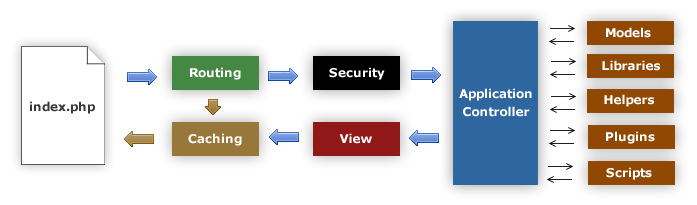
\includegraphics[width=1.0\columnwidth]{azienda/codeigniter_flow} 
	\caption{Flow chart di un'applicazione creata con Codeigniter.\\URL: \url{https://bit.ly/2QHOOrz}}
	\label{figura:flow-chart-codeigniter}
\end{figure}\\
Per quanto riguarda il \textit{frontend}, invece, viene utilizzato HTML5, CSS3 e Javascript (jQuery), senza usare framework che implementino Single Page Application (come React.js o Angular).\\\\\
Come server web, infine, vengono usati \textit{Apache2}, in caso di \textit{hosting} su piattaforma Linux, o  \textit{IIS}, in caso di \textit{hosting} su piattaforma Windows.\\\\
Per la realizzazione di siti web semplici, dove per semplici si intende senza esigenze di svolgimento di operazioni complesse, viene prediletto l'utilizzo di CMS, quali Wordpress (nel caso di blog, vetrine o forum) e OpenChart (nel caso di siti di e-commerce).
\\
\\
\subsubsection{DBMS}
Per lo sviluppo di prodotti software, WebPD si appoggia a due \gls{DBMS}: \textit{Microsoft SQL Server 2012} e \textit{MySQL Server}. Entrambi questi software sono \gls{RDBMS}, ma la scelta di utilizzare l'uno o l'altro dipende dalle caratteristiche del progetto, nello specifico: 
\begin{itemize}
	\item \textbf{Microsoft SQL Server} viene utilizzato nei progetti che prevedono un'ampia mole di dati da gestire e interrogazioni (query) complesse (come, ad esempio, CrociereRegalo.it), in quanto in tali contesti si è dimostrato mediamente più performante di \textit{MySQL}
	\cite{site:sqlcomparison};
	\item \textbf{MySQL Server} viene utilizzato il più possibile in caso il progetto non contenga una grossa mole di dati e/o interrogazioni complesse, in quanto non prevede costi di licenza (a differenza di \textit{SQL Server} che ha costi abbastanza elevati \cite{site:sqlserverpricing}) ed è multipiattaforma (attualmente disponibile per Linux, Windows e MacOS).
\end{itemize}

\subsection{Mobile}
Il \textit{know-how} accumulato da WebPD nella realizzazione di applicazioni web ha portato all'adozione del framework \textit{Cordova} (il cui schema di funzionamento è illustrato in Figura \ref{figura:funzionamento-cordova}) per la creazione di applicazioni mobile, il quale offre la possibilità di creare app ibride cross platform utilizzando HTML/CSS e Javascript. Tali applicazioni, grazie ad alcune interfacce messe a disposizione da Cordova, possono accedere alle funzionalità native del dispositivo, come fotocamera, storage o sensoristica varia (accelerometro, giroscopio e GPS, se presenti).

\begin{figure}[!h] 
	\centering 
	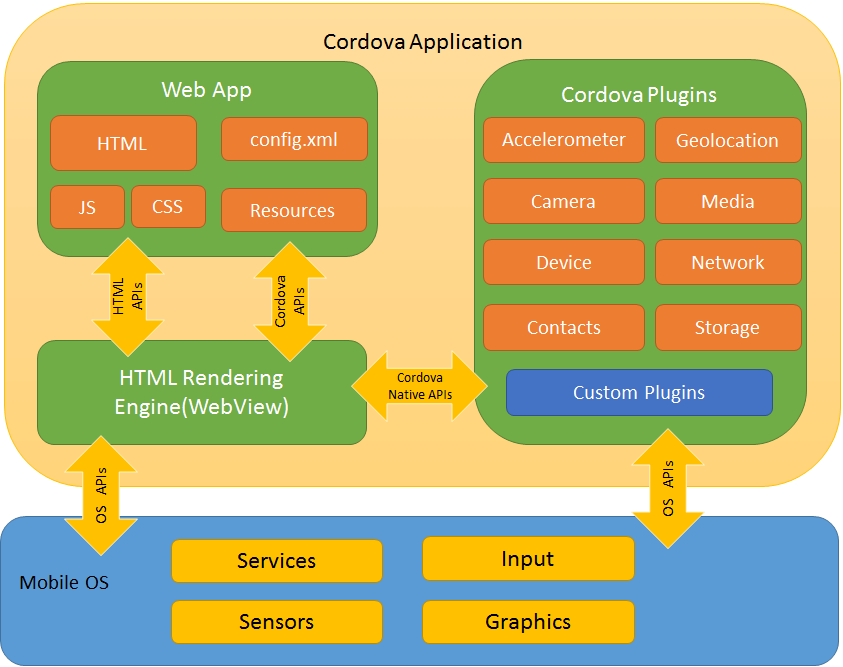
\includegraphics[width=0.6\columnwidth]{azienda/cordova_architettura} 
	\caption{Schema dell'architettura di un'app basata su Cordova.\\URL: \url{https://bit.ly/1TWONeg}}
	\label{figura:funzionamento-cordova}
\end{figure}

\subsection{Desktop}
La realizzazione di applicazioni desktop avviene attraverso l'utilizzo di due linguaggi: Java e Delphi.\\
Delphi viene usato soprattutto quando i programmi necessitano di manipolare grandi basi di dati, in quanto le applicazioni sono compilate in binario, quindi mediamente più performanti, e il linguaggio possiede numerose librerie che ne facilitano l'accesso.\\
Java, di contro, viene usato quando si ha l'esigenza di creare applicazioni cross-platform che non coinvolgano grandi volumi di dati.

\section{Processi aziendali}
\subsection{Ciclo di vita}
\label{sec:modello-evolutivo}
In WebPD, la \textit{way-of-working} inerente al ciclo di vita del software aderisce al \textit{modello Evolutivo}, le cui caratteristiche sono illustrate in Figura \ref{figura:modello-evolutivo}.\\
L'adozione di tale modello deriva principalmente dall'esigenza di doversi adattare alla mutevolezza dei requisiti. È un dato di fatto, purtroppo, che molto spesso neanche il cliente stesso ha chiare le proprie esigenze, quindi solo "toccando con mano" l'istanza del suo pensiero esso sa dire se effettivamente è ciò che fa per lui o no.\\
\begin{figure}[!h] 
	\centering 
	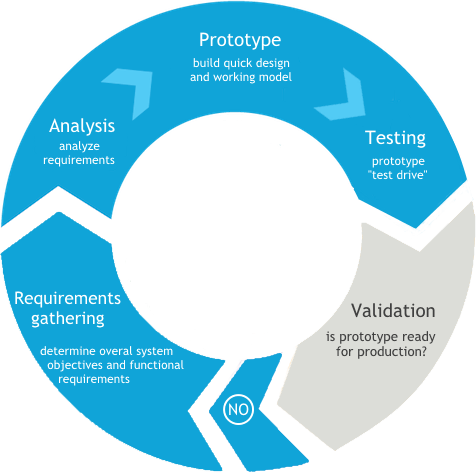
\includegraphics[width=0.6\columnwidth]{azienda/modello_evolutivo} 
	\caption{Schema del modello evolutivo. URL: \url{https://bit.ly/2N49cUI} }
	\label{figura:modello-evolutivo}
\end{figure}\\
Questo problema viene affrontato dal modello evolutivo, prevedendo che non venga effettuato solo un unico rilascio, ma che vengano creati prototipi, istanze di un sottoinsieme di requisiti del progetto, sottomessi poi al cliente. L'esito della valutazione dei prototipi può portare ad una rivisitazione dei requisiti inerenti alle funzionalità contenute in essi.\\
Nello specifico, il modello prevede le seguenti fasi :
\begin{enumerate}
	\item \textbf{Analisi e progettazione}, che viene fatta solo all'inizio del progetto e non si ripete;
	\item Per ogni prototipo:
		\begin{enumerate}
			\item \textbf{Progettazione di dettaglio} dei requisiti non implementati;
			\item \textbf{Sviluppo} di quanto appena progettato nel dettaglio;
			\item \textbf{Validazione} del prototipo appena sviluppato e, in base ai feedback del cliente, un'eventuale \textbf{revisione dei requisiti}.
		\end{enumerate}
	\item \textbf{Rilascio} della versione finale, corrispondente all'ultimo prototipo accettato dal proponente.
\end{enumerate}
Il modello evolutivo, inoltre, prevede la possibilità di avere più canali di sviluppo (ad esempio stabile, alpha, beta ecc.), utili per poter "sperimentare" nuove funzionalità senza andare ad intaccare la versione stabile del software.\\
Il problema principale di questo modello è che i tempi di sviluppo possono allungarsi notevolmente. La validazione da parte del cliente, infatti, è un'operazione che può richiedere molto tempo, durante il quale lo sviluppo non può proseguire. Inoltre, in caso di un cliente molto "indeciso", il numero di prototipi può aumentare, rischiando quindi che gli \glspl{incremento} si trasformino in \glspl{iterazione}.

\subsection{Miglioramento della qualità dei processi}
Nella way-of-working aziendale è presente una forte attenzione alla qualità dei processi. L'organizzazione interna di questi ultimi è incentrata sul principio del miglioramento continuo, grazie all'applicazione del Ciclo di Deming, conosciuto anche con l'acronimo PDCA. Tale acronimo contiene le iniziali delle quattro fasi in cui è possibile suddividere il processo di miglioramento: \begin{enumerate}
	\item \textbf{Plan}, ovvero pianificare, prima dell'inizio del processo, attraverso una attenta analisi di esso, eventuali problematiche e azioni di miglioramento;
	\item \textbf{Do}, ovvero eseguire il processo monitorato agendo secondo quanto pianificato nella fase precedente;
	\item \textbf{Check}, ovvero valutare (in modo retrospettivo) l'esito delle azioni derivanti da quanto pianificato all'inizio;
	\item \textbf{Act}, ovvero agire standardizzando ciò che è andato a buon fine e colmando le carenze.
\end{enumerate}
\begin{figure}[!h] 
	\centering 
	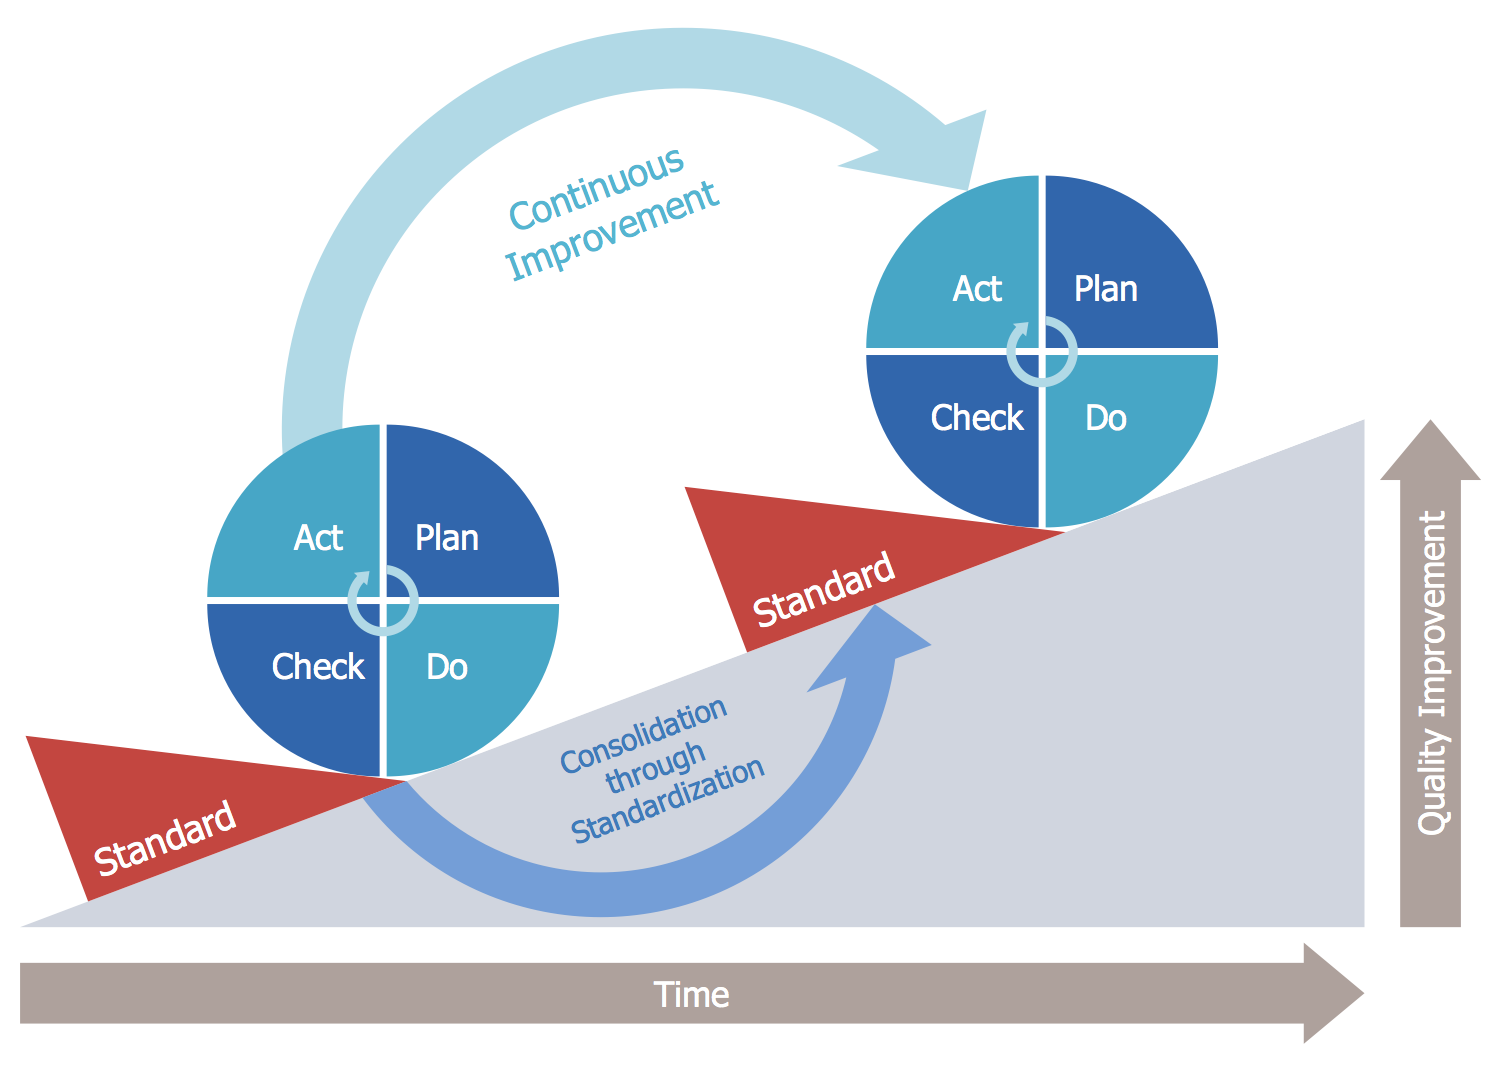
\includegraphics[width=0.6\columnwidth]{azienda/pdca} 
	\caption{Rappresentazione grafica del PDCA. URL: \url{https://bit.ly/2LP32TF} }
	\label{figura:pdca}
\end{figure}
A livello grafico, il PDCA è rappresentato attraverso un cerchio in movimento, che dichiara la ciclicità della sua applicazione.\\
In Figura \ref{figura:pdca} lo standard è rappresentato come un cuneo in quanto agisce da limite inferiore per la qualità. L'obiettivo del PDCA è quindi portare sempre più in alto la qualità dello standard.

\subsection{Strumenti a supporto dei processi}
\subsubsection{Gestione di progetto}
Per quanto riguarda gli strumenti di gestione di progetto, WebPD si affida a \textit{Trello}. 
Trello è uno software di amministrazione di progetto web-based, con numerose applicazioni per Android e iOS. Trello permette la creazione di una bacheca condivisa (come mostrato in Figura \ref{figura:trello}), organizzata in \textit{cards}, all'interno delle quali è possibile inserire dei compiti da svolgere (\textit{task}) e assegnare ciascuno di questi compiti una data di scadenza. \\
\begin{figure}[!h] 
	\centering 
	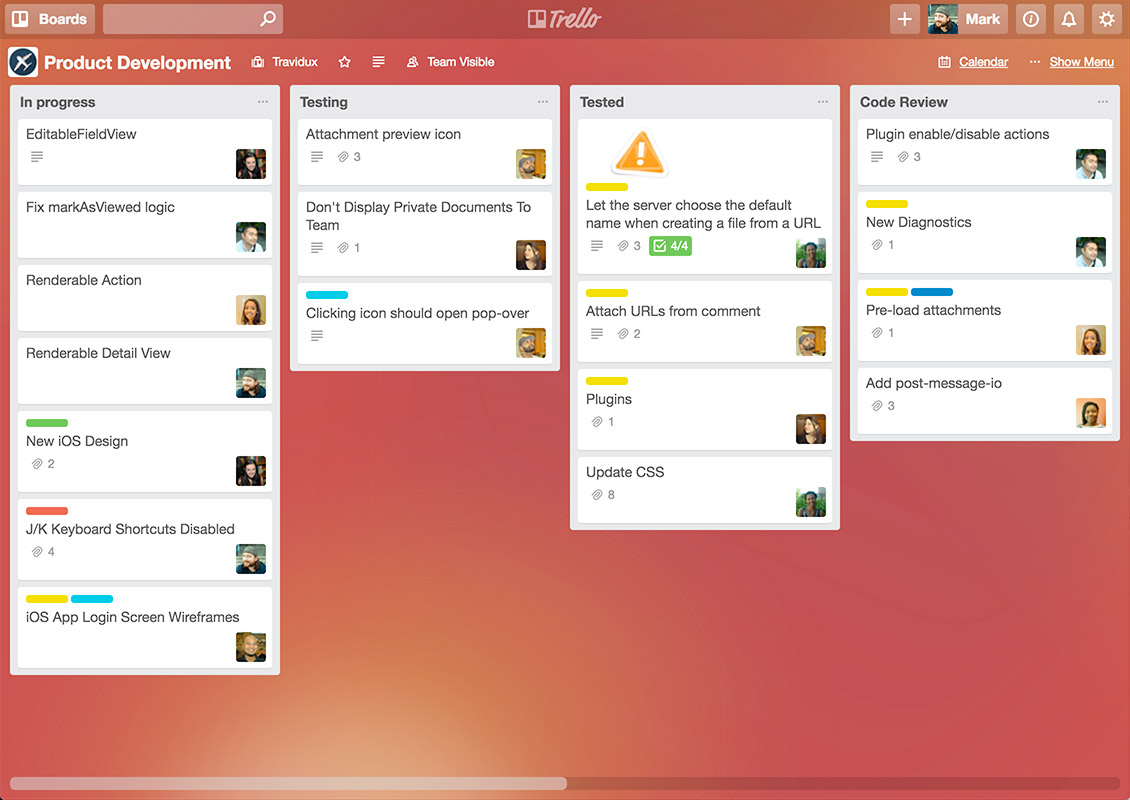
\includegraphics[width=0.8\columnwidth]{azienda/trello} 
	\caption{Screenshot dell'interfaccia web di Trello.}
	\label{figura:trello}
\end{figure}\\
Su ogni compito è possibile pubblicare dei commenti per, ad esempio, porre domande o fare determinate osservazioni e aggiungere checklist, etichette (tag) e allegati.\\ 
I \textit{task} possono inoltre essere agilmente spostati tra una \textit{card} e un'altra, funzionalità utile, ad esempio, per tenere quanto più pulita possibile la bacheca, nascondendo i \textit{task} già svolti o raggruppandoli in apposite \textit{cards} aventi funzione di storico.\\
Una feature molto interessante è la sincronizzazione in tempo reale delle modifiche, che permette a più persone di agire e collaborare sulla bacheca contemporaneamente, senza incorrere nel rischio di visualizzare o modificare dati non aggiornati.\\
Trello, infine, prevede anche numerosi \textit{Power-up}, ovvero estensioni (a pagamento) che permettono di interagire con numerosi servizi, quali, ad esempio, Google Drive, Onedrive, Google Calendar, GitHub, BitBucket, Slack ecc.\\
\\
Per avere una più immediata visualizzazione dell'andamento dei \textit{task}, assieme a Trello viene usato \textit{Trellogantt}. Quest'ultimo, come forse già suggerisce il nome, permette di visualizzare i dati contenuti in una bacheca di Trello sotto forma di diagrammi di Gantt, come mostrato in Figura \ref{figura:trellogantt}. Inoltre permette, con un semplice drag-and-drop, di modificare le date di scadenza dei vari task.\\

\begin{figure}[!h] 
	\centering 
	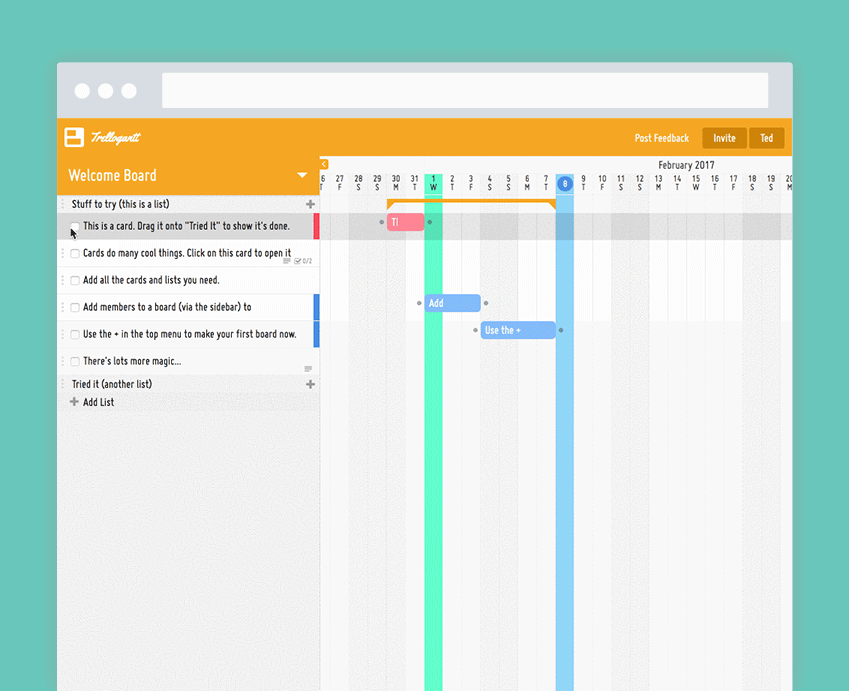
\includegraphics[width=0.8\columnwidth]{azienda/trellogantt} 
	\caption{Interfaccia di Trellogantt. URL: \url{https://bit.ly/2wysjgc} }
	\label{figura:trellogantt}
\end{figure}


\subsubsection{Gestione di versione}
WebPD, come strumento di versionamento, utilizza il software \textit{Git} (logo in Figura \ref{figura:logo-git}), probabilmente il più utilizzato nel suo campo.\\
\begin{figure}[!h] 
	\centering 
	
\includegraphics[width=0.3\columnwidth]{azienda/git} 
	\caption{Logo di Git }
	\label{figura:logo-git}
\end{figure}\\
 Le motivazioni che hanno spinto WebPD all'adozione di Git al posto del suo "antagonista" \textit{Subversion} (SVN) sono illustrate in Figura \ref{figura:differenze-git-svn}. In particolare\cite{site:svnvsgit}:
\begin{itemize}
	\item Decentralizzazione del repository: a differenza di Subversion, l'architettura di Git prevede che vi sia una copia dell'intero repository in ciascun client, in modo da poter effettuare \textit{commit} anche in assenza di una connessione verso il server (cosa non possibile con SVN);
	\item Velocità: le operazioni di commit sono molto spesso più veloci su Git in quanto vengono effettuate sulla copia locale del repository, ed è possibile poi inviarle al repository remoto (tramite \textit{push}) in un secondo momento, anche in blocco.
	\item Miglior gestione di branch e tag: in SVN, branch e tag sono copie dell'intero progetto (che quindi possono aumentare molto lo spazio richiesto dal repository sul server), mentre in Git sono semplicemente dei riferimenti ad una determinata commit.
\end{itemize}
\begin{figure}[!h] 
	\centering 
	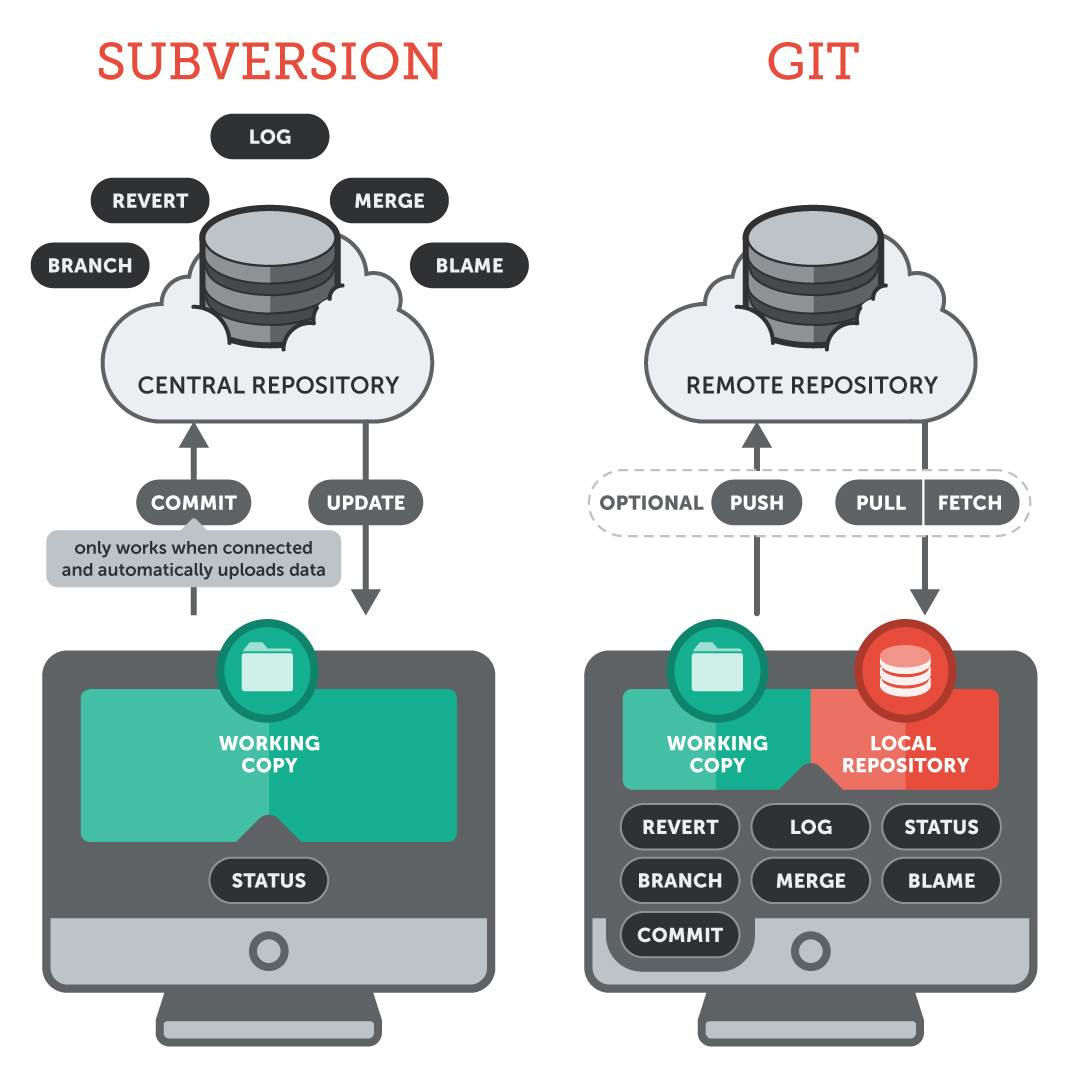
\includegraphics[width=0.8\columnwidth]{azienda/gitsvn} 
	\caption{Differenze tra Git e SVN. URL: \url{https://bit.ly/2ovUUOL} }
	\label{figura:differenze-git-svn}
\end{figure}
I repository contenenti tutti i progetti dell'azienda sono ospitati da un server Git privato, installato in uno dei server di WebPD. Tale scelta è stata fatta per essere quanto più tolleranti possibile ad un'eventuale assenza di connessione internet.

\subsubsection{Ambiente di sviluppo}
In azienda viene permesso a ciascun programmatore, in base alle sue preferenze, di scegliere l'ambiente di sviluppo che preferisce. In ogni caso ci sono degli strumenti generalmente preferiti, in base alla tecnologia utilizzata per sviluppare

\subsubsection{Sviluppo Web}
Per quanto riguarda lo sviluppo web, lo strumento più frequentemente utilizzato è \textit{Visual Studio Code} (la cui \textit{UI} è mostrata in Figura \ref{figura:vs-code}), un tool multi piattaforma sviluppato da Microsoft, che si pone in mezzo tra un \gls{ide} e un semplice editor di testo. Di base, infatti, non fornisce altro che la funzionalità di \textit{syntax highlight}, ma grazie a innumerevoli plugin, può acquisire, ad esempio, funzionalità avanzate di analisi statica. Inoltre si integra molto bene con Git, integrando degli strumenti per effettuare commit, push e merge.

\subsubsection{Sviluppo Mobile}
Dato che viene utilizzato \textit{Cordova}, le tecnologie utilizzate sono (quasi) analoghe a quelle utilizzate nello sviluppo web. Pertanto, anche in questo campo, \textit{Visual Studio Code}, coaudivato dagli adeguati plugin, rimane una scelta consueta. In alternativa, viene usato anche \textit{Jetbrains WebStorm}, un vero e proprio \gls{ide} che fornisce funzionalità avanzate di refactoring del codice e di linting.

\begin{figure}[!h] 
	\centering 
	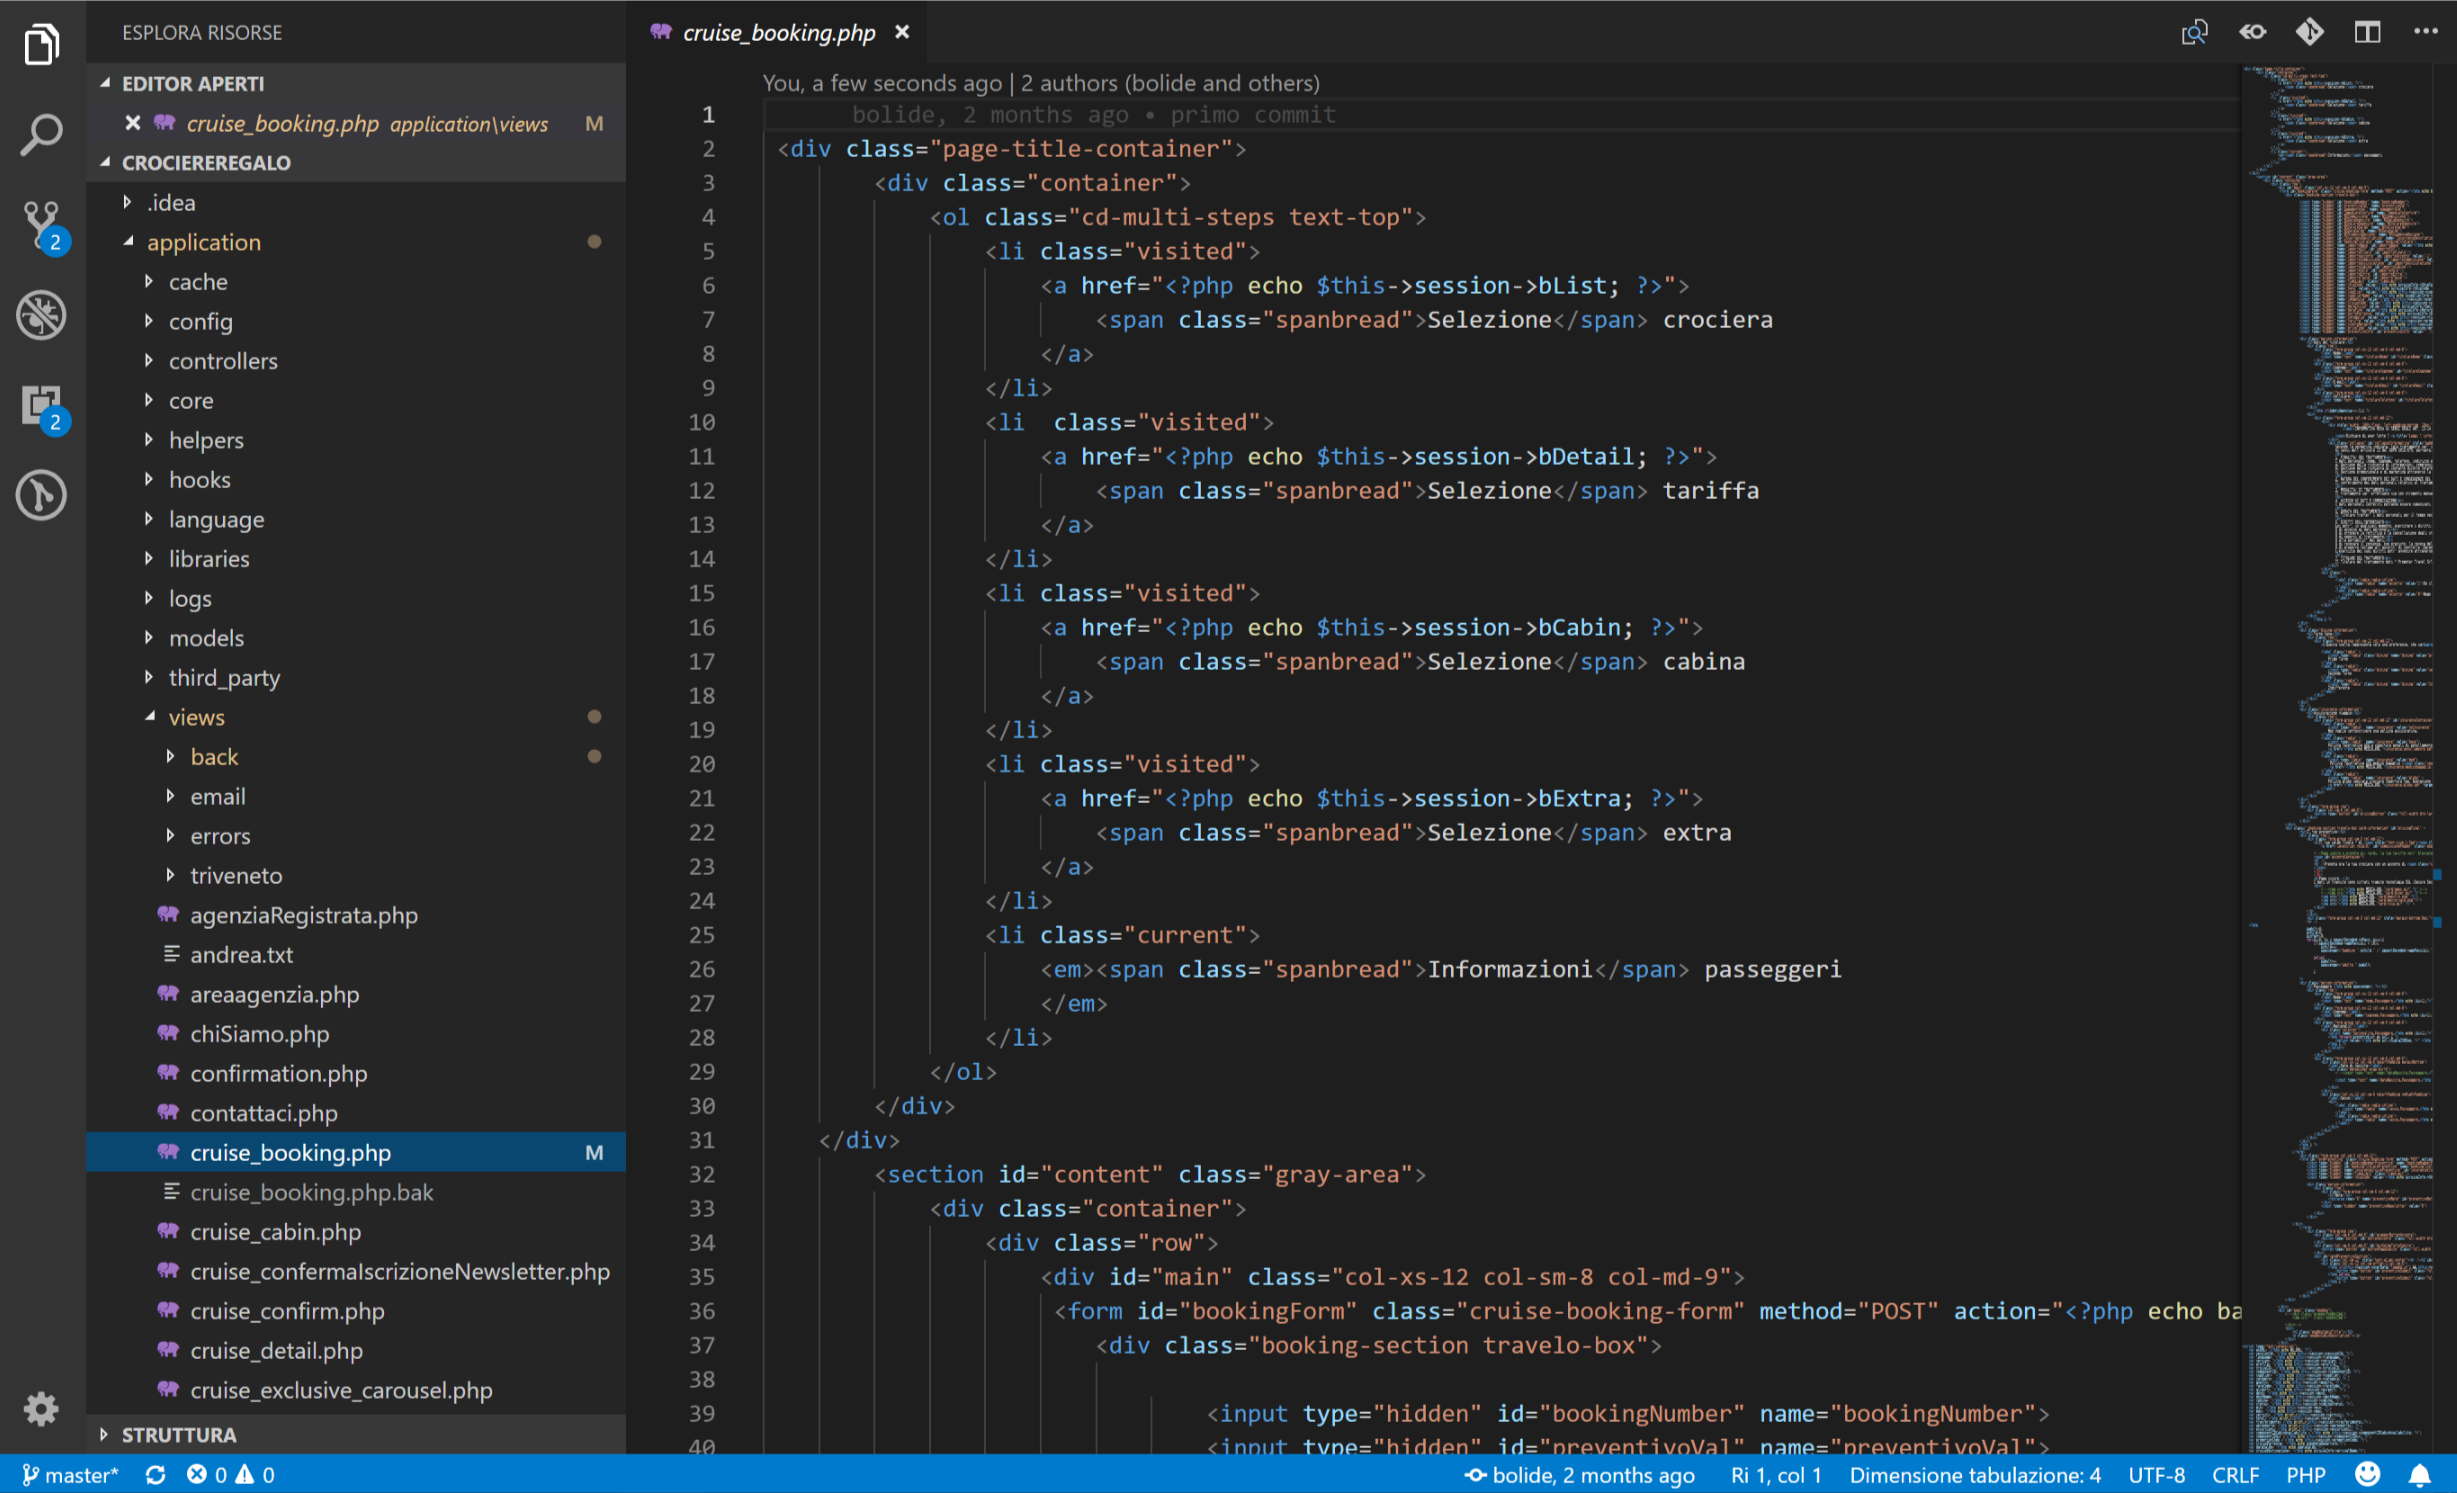
\includegraphics[width=0.8\columnwidth]{azienda/vscode} 
	\caption{Schermata di Visual Studio Code}
	\label{figura:vs-code}
\end{figure}

\subsubsection{Sviluppo Desktop}
Nello sviluppo di applicazioni desktop, bisogna fare una distinzione in base al linguaggio utilizzato. In caso si tratti di Java, l'\gls{ide} più comune è IntelliJ Idea, che offre strumenti di analisi "on-the-fly" e completamento e generazione automatica del codice. Discorso a parte per Delphi, in quanto, essendo una tecnologia proprietaria, si è vincolati all'\gls{ide} \textit{Embarcadero RAD Studio} che, tra le altre cose, ha un costo di licenza molto elevato (arriva a sforare i 6000 euro).

\section{Clientela}
La tipologia di cliente più comune per WebPD è la piccola-media impresa che vuole realizzare o ammodernare il suo sito web, vetrina o e-commerce che sia. Tale clientela proviene da numerosi settori, quali (per citarne alcuni) edile, farmaceutico, navale e turistico. WebPD possiede numerose soluzioni a portfolio, utili al cliente per capire meglio le sue esigenze, che, molto spesso, non sono ben chiare neanche a lui. Tutti i prodotti offerti, inoltre, sono altamente personalizzabili, in modo da concretizzare fedelmente quanto richiesto dal cliente.             % Processi
% !TEX encoding = UTF-8
% !TEX TS-program = pdflatex
% !TEX root = ../tesi.tex

%**************************************************************
\chapter{Descrizione dello stage}
\label{cap:descrizione-stage}
%**************************************************************

\section{Vantaggi per l'azienda}
WebPD trae diversi vantaggi dall'attività di stage curricolare che è stata disposta ad ospitare.\\
\\
Primo su tutti, l'inserimento in azienda, seppur solo per un paio di mesi, di un nuovo membro del personale, mai entrato in contatto con l'azienda. Ciò, in primis, ha permesso di distribuire il carico di lavoro tra più persone, permettendo di accelerare lo sviluppo sui progetti in cantiere. Inoltre, l'introduzione nel team di una persona completamente esterna all'azienda, ha portato un ulteriore punto di vista all'interno del team di sviluppo. Tale punto di vista si è dimostrato utile nel tentativo di risoluzione di alcuni problemi software "cronici" (come la lentezza di esecuzione delle query, problema che verrà descritto nel dettaglio nel prossimo capitolo), permettendo un ragionamento fuori dagli schemi mentali dell'ideatore di tale software.\\
\\
In secondo luogo, ha permesso all'azienda di esplorare nuovi canoni stilistici per alcuni suoi prodotti a costo zero, come nel caso del restyling della homepage del sito CrociereRegalo (descritta anch'essa nel prossimo capitolo), senza quindi il rischio di sacrificare il lavoro (e la retribuzione) di un membro del personale.

\section{Presentazione del progetto}
L'obiettivo di questo stage è permettere a WebPD di completare la riscrittura del sito CrociereRegalo.it. Tale sito, infatti, prima dell'ingresso di Primarete tra le quote di WebPD, era stato realizzato e mantenuto da WebCola, una web agency con la quale Primarete aveva stretto una partnership commerciale, che si è appunto interrotta nel 2015.\\
Secondo gli accordi presi, il sorgente del sito era di proprietà di WebCola, pertanto non è stato possibile per WebPD procedere ad una semplice modifica/aggiornamento di qualcosa già esistente. Il vecchio sito (il cui aspetto è mostrato in Figura \ref{figura:vecchio-sito}), inoltre, non era responsive e, dai dati di Google Analytics è emerso che la maggior parte delle visite avveniva da dispositivi mobili. \\
La problematica maggiore, comunque, si sono rivelati gli accordi presi con le varie compagnie di crociera (MSC, Costa, Royal Caribbean, Celebrity e Azamara): tali accordi, infatti, erano stati presi da WebCola in nome e per conto suo, quindi WebPD si è vista obbligata a ristabilirli.
\begin{figure}[!h] 
	\centering 
	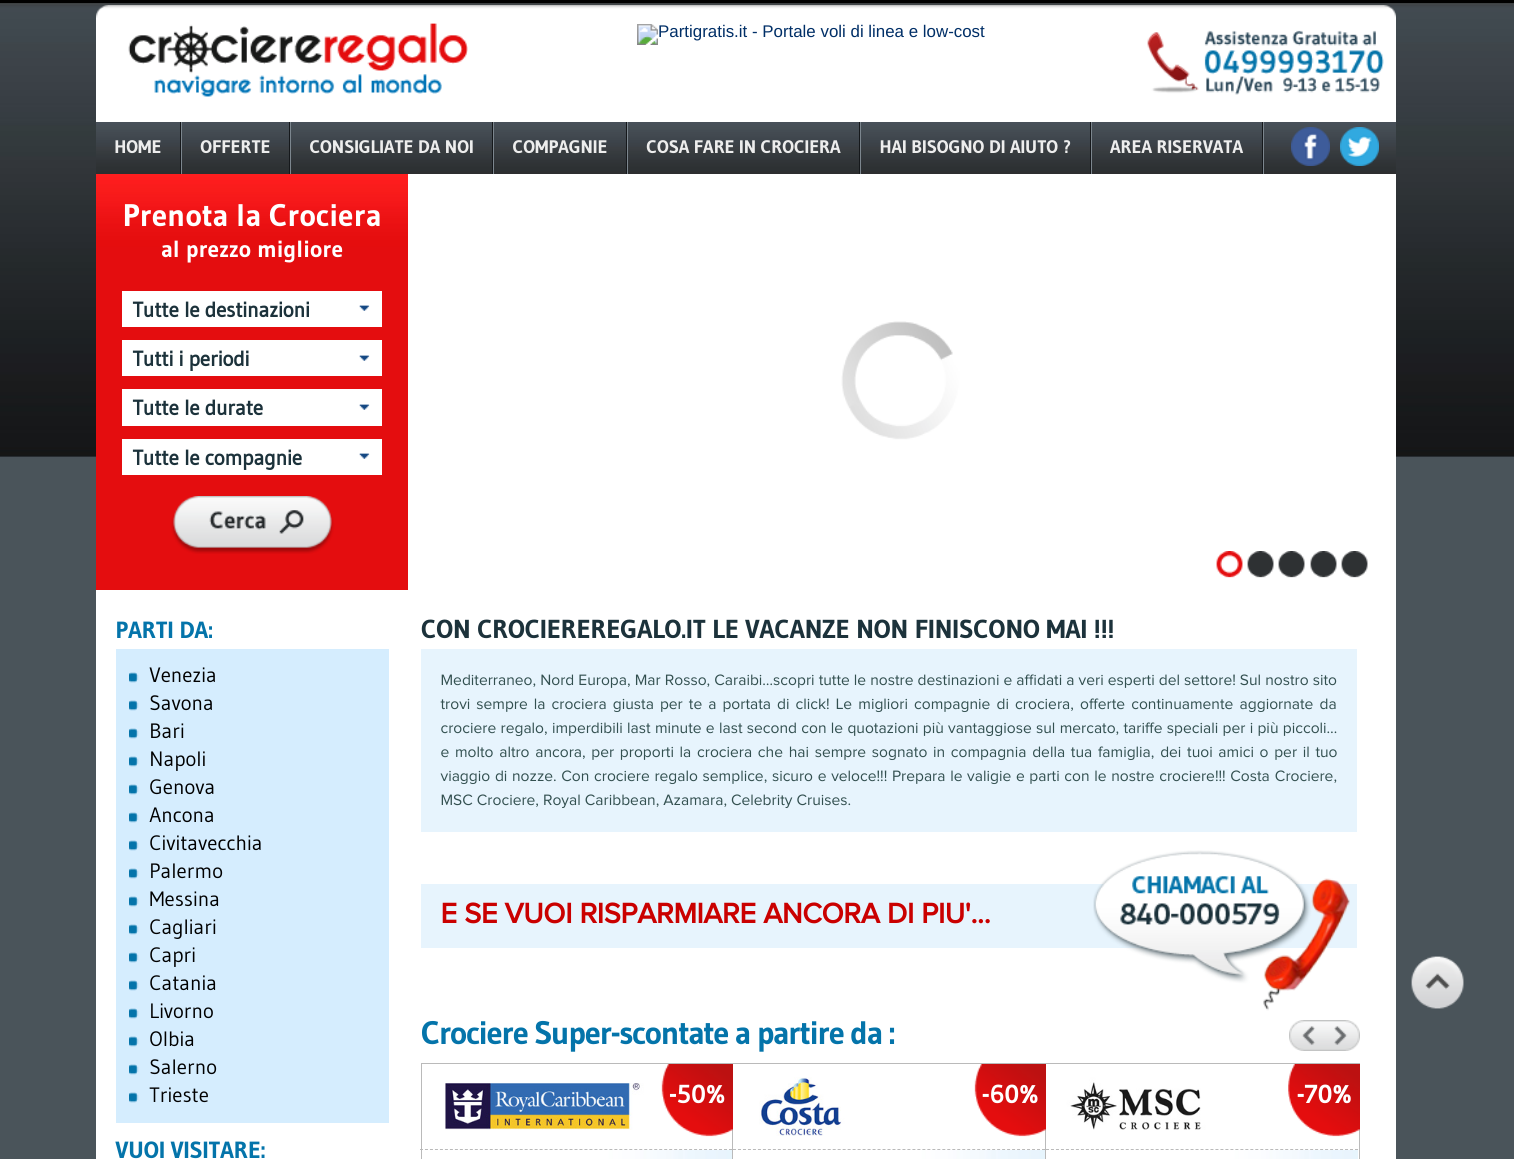
\includegraphics[width=.9\columnwidth]{stage/webcola_crociereregalo} 
	\caption{Screenshot della versione di CrociereRegalo sviluppata da WebCola}
	\label{figura:vecchio-sito}
\end{figure}\\
Dal 2015 fino ad luglio 2018, WebPD è riuscita a creare un \bookingEngine\hphantom{i}che interagisse con \Gls{api} e \glspl{webservice} forniti da Costa e MSC, permettendo di acquistare una crociera, pagando tramite un payment gateway fornito dal consorzio TVB (Triveneto Bassilichi). La soluzione realizzata, però, aveva grossi problemi di prestazioni (ad esempio la homepage del sito aveva un tempo di risposta medio di 7 secondi, a cui poi doveva essere sommato il tempo di download della risposta, rendering grafico ed esecuzione del codice Javascript presente) e mancava di alcune funzionalità, come la possibilità di vendere tariffe \textit{vuoto per pieno}. Esse non sono altro che posti (cabine) acquistati da un'agenzia viaggi (nel caso in esame, Primarete) ad un prezzo scontato e rivenduti poi ai privati.
\\
Lo stage ha come obiettivo il completamento e l'ampliamento delle funzionalità offerte dal \bookingEngine\hphantom{i}alla base di CrociereRegalo. Più nello specifico, lo stage si propone di svolgere le attività descritte in seguito.

\subsection{Studio di funzionamento del \bookingEngine}
La parte introduttiva dello stage si pone come obiettivo quello di analizzare e capire il funzionamento del \bookingEngine. Infatti quest'ultimo è realizzato tramite il \gls{framework} \textit{Codeigniter}, e, quindi, gode di una struttura delle classi particolare, come anche il modo in cui vengono gestiti gli URL. Inoltre, usando come \gls{DBMS} il software \textit{Microsoft SQL Server}, il linguaggio utilizzato per le interazioni con il database è \textit{Transact SQL}, un dialetto di \textit{SQL}, con il quale è necessario prendere confidenza.

\subsection{Ottimizzazione delle performance del \bookingEngine}
Come accennato precedentemente, il \bookingEngine\hphantom{i}ha grossi problemi di prestazioni. Ciò è dovuto principalmente alla grande mole di dati contenuta nel database, che deve essere interrogato molteplici volte ad ogni richiesta HTTP ricevuta. Gli scopi di questa fase dello stage sono i seguenti:
\begin{enumerate}
	\item Ottimizzare il database in modo che le interrogazioni risultino più veloci. A tale scopo \textit{SQL Server} fornisce una funzionalità chiamata \textit{Database Engine Tuning Advisor} (mostrata in Figura \ref{figura:database-tuning-engine}), che permette, sottoponendole delle query da analizzare, di suggerire la creazione di eventuali indici, in modo da aumentare le performance delle interrogazioni;
	\item Valutare se implementare o meno (e in caso positivo, farlo) un meccanismo di caching dei risultati delle query, in modo da diminuire le interrogazioni al database il più possibile.
\end{enumerate}

\begin{figure}[!h] 
	\centering 
	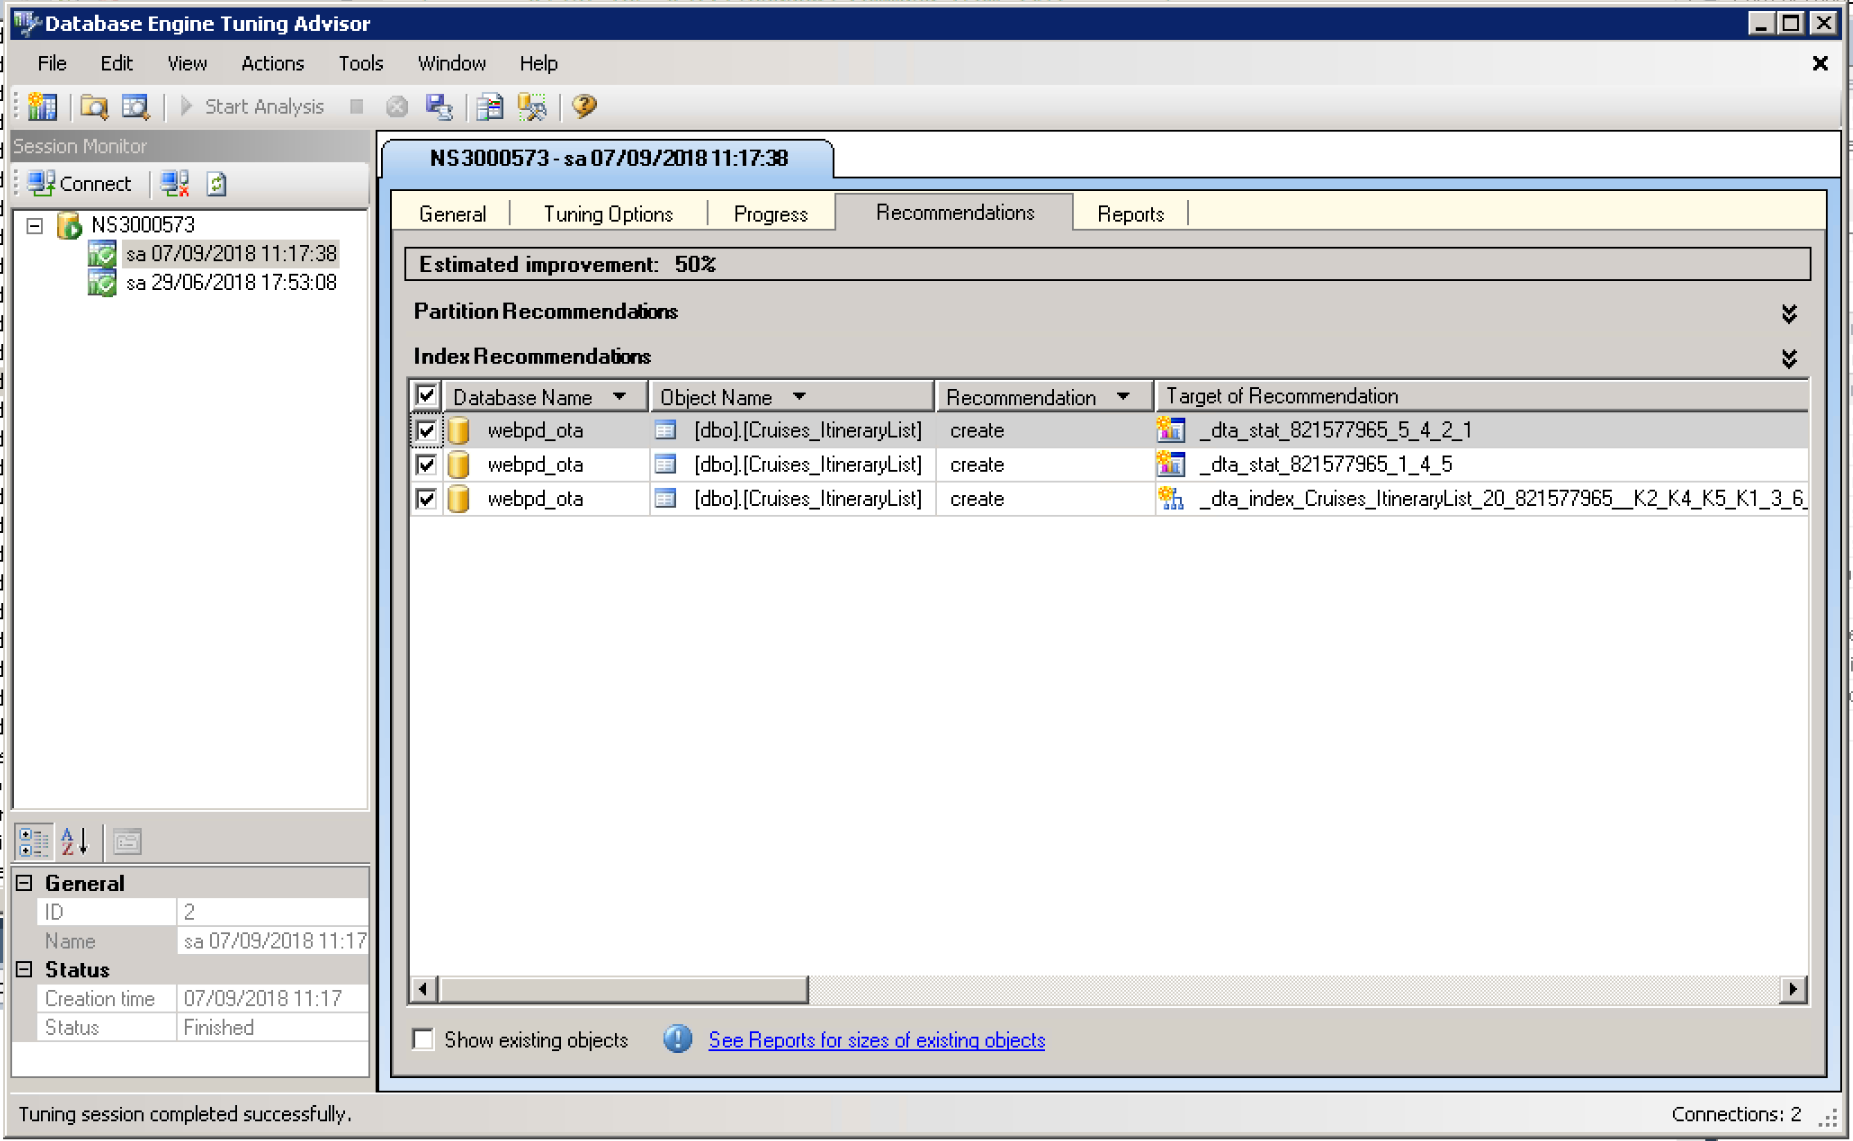
\includegraphics[width=.9\columnwidth]{stage/tuning_query} 
	\caption{Screenshot del tool Database Tuning Engine Advisor utilizzato per l'ottimizzazione delle query}
	\label{figura:database-tuning-engine}
\end{figure}

\subsection{Integrazione delle tariffe \textit{vuoto per pieno}}
Il partner Primarete ha espresso l'esigenza di poter vendere le proprie tariffe \textit{vuoto per pieno} attraverso il \bookingEngine. Come specificato precedentemente, esse sono dei gruppi di cabine acquistate "al buio" da un'agenzia viaggio ad un prezzo scontato (in quanto ne vengono acquistate più di una in blocco), che poi verranno rivendute dall'agenzia stessa ai clienti. Ovviamente, il guadagno dell'agenzia viaggi è rappresentato dalla differenza tra il prezzo di vendita della cabina e quello di acquisto.\\
Il problema è che le cabine associate al \textit{vuoto per pieno}, agli occhi dei \glspl{webservice} delle varie compagnie di crociera, risultano prenotate, quindi non disponibili: è necessario modificare il flusso di prenotazione del \bookingEngine\hphantom{i}permettendo di inserirvi anche i gruppi di cabine acquistate tramite tariffa \textit{vuoto per pieno}, oltre a quelle ancora effettivamente disponibili; tale modifica dovrà essere fatta sia a livello backend che frontend.

\subsection{Aggiunta delle tariffe di un nuovo fornitore}
La versione di CrociereRegalo sviluppata da WebCola integrava, oltre alle crociere di MSC e Costa, anche quelle di Royal Caribbean (e controllate, ovvero Celebrity e Azamara). Lo stage, quindi, si prefigge di ripristinare questa funzionalità anche sulla nuova versione del \bookingEngine\hphantom{i}CrociereRegalo reintroducendo nel flusso di prenotazione le crociere del gruppo Royal, tramite l'integrazione dei \glspl{webservice} forniti da IST (Fibos). Tale integrazione comporterà modifiche sia alla parte frontend che alla parte backend del \bookingEngine


\subsection{Altri interventi minori}
\label{section:altri-interventi-minori}
La fase conclusiva dello stage si prefigge di svolgere interventi minori su CrociereRegalo, per migliorarne la \gls{seo} ed in generale l'accessibilità, soprattutto dai dispositivi mobili.

\section{Obiettivi dello stage}
In fase di definizione contenutistica dello stage, i punti sopra descritti sono stati distribuiti in obiettivi aventi tre livelli di priorità, tenendo conto anche del numero di ore ridotto (circa 310) a disposizione dello stagista, identificati dalle seguenti sigle:
\begin{itemize}
	\item \textbf{Ob} per gli obiettivi obbligatori, vincolanti in quanto obiettivo primario richiesto dal committente;
	\item \textbf{D} per gli obiettivi desiderabili, non vincolanti o strettamente necessari, ma dal riconoscibile valore aggiunto;
	\item \textbf{Op} per gli obiettivi opzionali, rappresentanti valore aggiunto non strettamente competitivo.
\end{itemize}

\begin{longtable}{
		@{}
		>{\raggedright}p{.5cm}
		p{10.5cm}
		>{\raggedleft}p{0.2cm}@{}
		>{\raggedright}p{0.2cm}
		p{8.5cm}
		@{}} 
	\hline
	\multicolumn{2}{|c|}{\textbf{Obbligatori}}\\
	\hline
	Ob1 & Interazione con il database SQL Server attraverso le librerie del \gls{framework} Codeigniter\\
	\hline
	Ob2 & Realizzazione integrazione flat-file di un nuovo fornitore con il Data Exchange del \bookingEngine\\
	\hline
	Ob3 & Aggiunta prodotti e tariffe del nuovo fornitore ai risultati della ricerca lato Front-End del \bookingEngine\\
	\hline
	Ob4 & Esecuzione test e redazione documentazione sul lavoro svolto\\
	\hline
	\multicolumn{2}{|c|}{\textbf{Desiderabili}}\\
	\hline
	D1 & Realizzazione del registro carichi/scarichi tariffe “vuoto per pieno” come	funzionalità lato Back-End del \bookingEngine\\
	\hline
	D2 & Interrogazione web-service in tempo reale per sincronizzare prezzi e disponibilità del nuovo fornitore con il Data Exchange\\
	\hline
	D3 & Realizzazione conferma prenotazione al fornitore come funzionalità lato Front-End del \bookingEngine\\
	\hline
	\multicolumn{2}{|c|}{\textbf{Opzionali}}\\
	\hline
	Op1 & Analisi e realizzazione di nuove funzionalità\\
	\hline
\end{longtable}

\section{Vincoli}
\subsection{Vincoli metodologici}
In accordo con il tutor aziendale, lo stage si è svolto presso la sede dell'azienda. Questa scelta è stata fatta principalmente per due motivi:
\begin{itemize}
	\item agevolare la comprensione, da parte dello stagista, delle dinamiche aziendali e l'interazione con il proponente del progetto CrociereRegalo (WebPD e Primarete hanno l'ufficio all'interno dello stesso palazzo);
	\item favorire al massimo l'interazione tra stagista e tutor aziendale, evitando ritardi di risposta, problematica che invece può avere il \textit{remote-working}.
\end{itemize}
Inoltre è stato deciso che, al raggiungimento di ogni obiettivo prefissato, lo stagista avrebbe dovuto redarre una breve relazione, descrivendo le problematiche affrontate, le scelte adoperate e il risultato ottenuto. Tali relazioni, poi, fungeranno da materiale ausiliario per la presentazione delle nuove funzionalità al proponente.\\
Infine, è stato posto come obbligo che tutto il lavoro prodotto dallo stagista sia sottoposto a versionamento, quindi caricato in un repository Git dedicato, ospitato sul server aziendale.

\subsection{Vincoli temporali}
\label{sec:vincoli-temporali}
Lo stage ha una durata prevista di \textit{310} ore complessive, distribuite in 9 settimane da 34 ore lavorative ciascuna (ad esclusione della prima, da 38 ore). L'orario di lavoro concordato con il tutor aziendale è stato dal Lunedì al Giovedì dalle 09:00 alle 18:30, con 1 ora di pausa pranzo. \\
Prima dell'inizio dello stage è stata definita, nel piano di lavoro, una scansione temporale delle attività con granularità settimanale così definita:
\begin{itemize}
	\item \textbf{Prima settimana}: formazione sulle tecnologie utilizzate dal \bookingEngine\hphantom{i}CrociereRegalo, con particolare attenzione alla libreria \textit{Codeigniter} e al \gls{DBMS} \textit{Microsoft SQL Server};
	\item \textbf{Seconda settimana}: Proseguimento delle attività di formazione iniziate la prima settimana. Ottimizzazione del database tramite gli strumenti forniti da SQL Server;
	\item \textbf{Terza settimana}: Ottimizzazione del sito tramite implementazione della cache delle query. Studio e progettazione dell'aggiunta delle tariffe \textit{vuoto per pieno} al flusso dati del \bookingEngine;
	\item \textbf{Quarta settimana}: Realizzazione, test e redazione di documentazione di quanto progettato la settimana precedente;
	\item \textbf{Quinta settimana}: Studio e progettazione dell'integrazione dati forniti dal sistema FIBOS (Royal);
	\item \textbf{Sesta settimana}: Realizzazione dell'integrazione di navi, porti, itinerari, categorie di cabina e prezzi attraverso interrogazioni schedulate ai \glspl{webservice} FIBOS;
	\item \textbf{Settima settimana}: Realizzazione, test e redazione di documentazione di quanto progettato la settimana precedente;
	\item \textbf{Ottava settimana}: Studio e progettazione dell'aggiunta delle tariffe Royal al flusso di prenotazione;
	\item \textbf{Nona settimana}: Realizzazione, test e redazione di documentazione inerente a quanto progettato la settimana precedente.
\end{itemize}

\subsection{Vincoli tecnologici}
A livello implementativo, l'azienda non ha imposto precisi vincoli, se non quello di aderire il quanto più possibile ai paradigmi di programmazione già preesistenti ed applicare del buon senso a quanto si intende realizzare. Ciò principalmente significa dovrà essere adottato un design pattern \gls{mvc} (il cui schema di funzionamento è mostrato in Figura \ref{figura:mvc}), intrinseco di \textit{Codeigniter}, e cercare di creare del codice che 
sia quanto più manutenibile possibile. Ovviamente, quanto realizzato avrebbe dovuto girare correttamente sull'ambiente di esecuzione già utilizzato, ovvero \textit{PHP 7.1} su \textit{Windows Server 2008 R2}, \textit{IIS} come web server e \textit{SQL Server 2012} come \textit{\gls{DBMS}}.
\begin{figure}[!h] 
	\centering 
	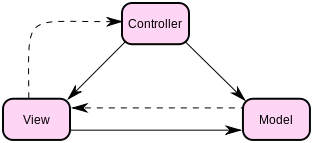
\includegraphics[width=0.6\columnwidth]{stage/mvc} 
	\caption{Schema UML dell'architettura \gls{mvc}. URL: \url{https://bit.ly/2wPfE8E} }
	\label{figura:mvc}
\end{figure}\\

\subsection{La mia scelta}
È da quando ero alle scuole elementari che ho la passione per l'informatica, ed è proprio per coltivare questa passione che ho scelto il cammino di studi che sto portando a termine in questo momento. Sono sempre stato affascinato dalla programmazione web, e il primo linguaggio in cui ho imparato a programmare (da autodidatta, nell'ormai lontano 2012) è stato \textit{PHP}.\\
Dal 2012 ad oggi ho svolto numerosi progetti utilizzando l'accoppiata HTML/PHP, coadiuvata da Javascript e SQL (MySQL). Molti di questi progetti sono stati solo "esercizi di stile", utili per mettermi alla prova, per mettere alla prova quanto imparato e per cercare di ampliare più possibile le mie conoscenze ed abilità nel campo della programmazione. Alcuni progetti, però, sono anche stati adottati e utilizzati da aziende, il ché mi ha regalato non poche soddisfazioni. In ogni caso, ho sempre fatto il programmatore a livello amatoriale.\\
Ho scelto di svolgere questo stage per inserire un nuovo tassello nel percorso di crescita personale che sto intraprendendo: volevo confrontare il mio modo "amatoriale" di lavorare con una way-of-working aziendale. Essendo io già abbastanza familiare con le tecnologie utilizzate da \textit{WebPD}, avrei potuto effettuare un confronto molto diretto tra la metodologia di lavoro aziendale e la mia.              % Kick-Off
% !TEX encoding = UTF-8
% !TEX TS-program = pdflatex
% !TEX root = ../tesi.tex

%**************************************************************
\chapter{Resoconto dello stage}
\label{cap:resoconto-stage}
%**************************************************************

\intro{In questo capitolo verranno descritte le attività svolte durante lo stage. Per ogni attività si cercherà di descrivere il problema affrontato, le scelte effettuate ed i test svolti.}\\

%\section{Pianificazione}
%La prima attività svolta, in realtà ancora prima dell'inizio dello stage stesso, è stata quella di pianificare il lavoro da svolgere. Tale %pianificazione è stata concordata tra il tutor aziendale e il sottoscritto, ed è esposta nella sezione \ref{sec:vincoli-temporali} a pagina %\pageref{sec:vincoli-temporali} di questo documento.\\
%Tale pianificazione, però, è stata "aggiustata" (ma mai stravolta) in base a quanto svolto settimana per settimana, decidendo di dedicare più o meno ore ad una determinata attività.\\
%Al termine di ogni settimana, periodo coincidente con il raggiungimento di un obiettivo, infine, è stato deciso che avrei dovuto redarre una %breve relazione, con lo scopo di documentare il lavoro svolto. Tali relazioni, inoltre, sono servite come materiale ausiliario per la %presentazione delle nuove funzionalità sviluppate al proponente. Infine, terminati tutti gli obiettivi e in caso di approvazione da parte del %tutor e del proponente, avrei dovuto trasferire il lavoro svolto dall'ambiente di sviluppo a quello di produzione.

\section{Scelte tecnologiche}
A livello tecnologico, datosi che il \bookingEngine\hphantom{i}è basato sullo stack che in azienda viene chiamato \gls{wisp}, sono stato obbligato ad utilizzare \textit{PHP} su \gls{framework} \textit{Codeigniter} per la parte \textit{backend}, \textit{HTML5}, \textit{CSS3}, \textit{Javascript} (principalmente utilizzando \gls{jquery}) per quanto riguarda il \textit{frontend}. Infine, per la comunicazione tra \textit{backend} e \textit{frontend} ho adoperato richieste \gls{ajax} con \gls{json} come formato per lo scambio di dati. Come ambiente di sviluppo ho deciso di usare \textit{Visual Studio Code} per via della sua semplicità e possibilità di personalizzazione. Infine, tutto il lavoro che ho svolto è stato sottoposto a versionamento utilizzando il server \textit{Git} dell'azienda. 

\section{Funzionamento e struttura del \bookingEngine}
Appena iniziato lo stage, mi sono subito dedicato all'analisi della struttura di CrociereRegalo, grazie anche (soprattutto all'inizio) all'aiuto del mio tutor. 
\subsection{Funzionalità}
CrociereRegalo è un motore di ricerca di crociere. Permette di trovare una determinata crociera utilizzando dei filtri di ricerca per area geografica (ad esempio Caraibi, Mediterraneo, Nord Europa), per data di partenza con granularità mensile (ad esempio Settembre 2018), per intervalli di durata (da 1-6, 7-8, 9-12 o più di 12 giorni) e per compagnia di crociera (ad esempio MSC Crociere). Per capire bene il suo funzionamento è stato necessario apprendere alcuni termini tecnici affini all'ambiente croceristico, come:
\begin{itemize}
	\item \textbf{Itinerario}: definisce il percorso che fa una crociera (ad esempio "Barcellona, Ajaccio, Civitavecchia, Barcellona"). Nell'arco di un periodo di tempo vi possono essere molteplici crociere percorrenti un singolo itinerario. Ogni itinerario è identificato da un codice che lo contraddistingue univocamente, e la durata dell'itinerario è una proprietà intrinseca (ovvero, all'interno di una compagnia di crociera, non esistono due itinerari che svolgono lo stesso percorso mettendoci tempi diversi). Ciascun itinerario ha 0 o più partenze nell'arco di un anno;
	\item \textbf{Cabina}: una stanza di una nave da crociera. Esistono varie categorie di cabina, differenziate in base alla grandezza, al posizionamento (ad esempio le cabine interne alla nave, senza quindi finestre, che sono quelle più economiche). Quando si effettua una prenotazione, non viene prenotato un posto letto ma viene prenotata un'intera cabina;
	\item \textbf{Opzione}: consiste nel blocco del prezzo di una cabina per un periodo di tempo che varia in base al fornitore, ma che di solito si attesta tra le 24 e le 72 ore. Tale prezzo infatti, analogamente per quanto avviene con i biglietti aerei, aumenta all'aumentare delle prenotazioni (quindi al passare del tempo).

\end{itemize}
CrociereRegalo permette di selezionare un itinerario, vederne le partenze, categorie di cabina disponibili e prezzi e poi prenotare od opzionare una cabina. 

\subsection{OTA e DataExchange}
Mi è stato spiegato che il \bookingEngine, in realtà, era spezzato in due parti dipendenti l'una dall'altra: \textbf{OTA} (disponibile all'indirizzo \cite{site:crociereregalo}) e \textbf{DataExchange} (disponibile all'indirizzo \cite{site:dataexchange}). L'idea alla base di questa divisione è che la parte \textit{OTA} rappresenti il sito web vero e proprio, con il quale l'internauta si affaccia, mentre la parte \textit{DataExchange} serva per l'interazione tra \textit{OTA} e \glspl{webservice} dei vari fornitori (dove per fornitori si intendono le varie compagnie di crociera). 

\subsection{Interazione tra OTA e DataExchange}
\textit{OTA} e \textit{DataExchange} sono dipendenti l'uno dall'altro, ma hanno due database separati. Questo, fondamentalmente, avviene perchè i dati provenienti da i vari fornitori hanno formati diversi, che devono quindi essere uniformati per poter essere processati secondo una logica più indipendente possibile. Il compito del \textit{DataExchange} è proprio questo: interrogare i \glspl{webservice} dei vari fornitori, ricevere i dati, elaborarli, uniformarli e passarli ad \textit{OTA}.\\
Vi sono due possibili interazioni tra \textit{OTA} e \textit{DataExchange}
\begin{itemize}
	\item Interazione \textbf{schedulata} (illustrata in Figura \ref{figura:integrazione-schedulata}), che avviene circa 3 volte al giorno, il cui compito è sincronizzare i cataloghi (chiamati anche \textit{flatfile}) dei vari fornitori per rendere disponibili le (eventuali) modifiche alla parte \textit{OTA} del \bookingEngine. \\Quando un visitatore del sito CrociereRegalo cerca una crociera, tale ricerca avviene interrogando i cataloghi presenti nel database della parte \textit{OTA}, senza quindi interrogare i \glspl{webservice} delle compagnie di crociera (per motivi di prestazione dovuti all'ingente mole di dati da elaborare). I cataloghi, quindi, vengono scaricati nel DataExchange, elaborati (uniformati) e poi sincronizzati con il database di OTA; la procedura di sincronizzazione viene chiamata \textbf{Integrazione}. L'integrazione avviene attraverso l'invocazione (grazie allo scheduler di \textit{Windows Server}) che, grazie ad una chiamata \textit{HTTP} ad una particolare pagina del DataExchange, invoca la procedura di integrazione dati.
	\begin{figure}[!h] 
		\centering 
		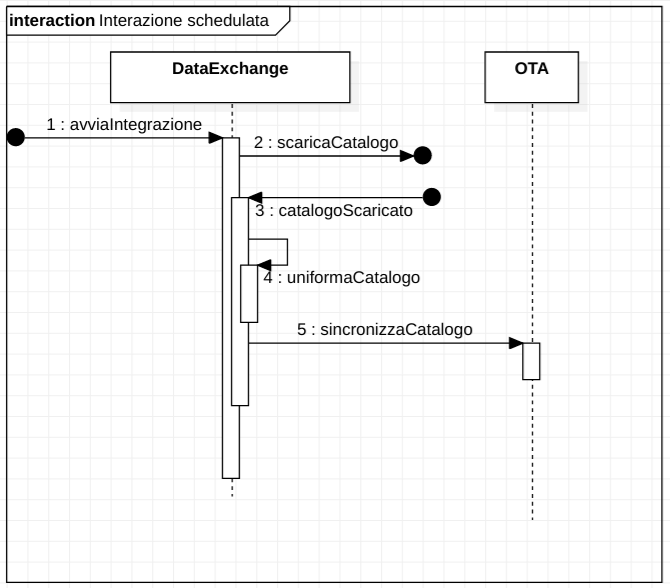
\includegraphics[width=.75\columnwidth]{attivita/interazione_schedulata} 
		\caption{Schema dell'integrazione schedulata DataExchange-OTA.}
		\label{figura:integrazione-schedulata}
	\end{figure}
	\item Interazione \textbf{real-time} (rappresentata in Figura \ref{figura:integrazione-realtime}), che avviene durante tutto il flusso di prenotazione di una cabina (che analizzerò in seguito). Tale flusso deve per forza disporre di dati aggiornati in tempo reale, altrimenti potrebbero verificarsi problemi in fase di prenotazione (come la prenotazione di una cabina non più disponibile). L'interazione in tempo reale avviene attraverso delle chiamate \textit{HTTP} (\gls{ajax}) effettuate nel momento del bisogno dall'\textit{OTA} al \textit{DataExchange}, attraverso lo scambio di dati in formato \gls{json}.
	\begin{figure}[!h] 
		\centering 
		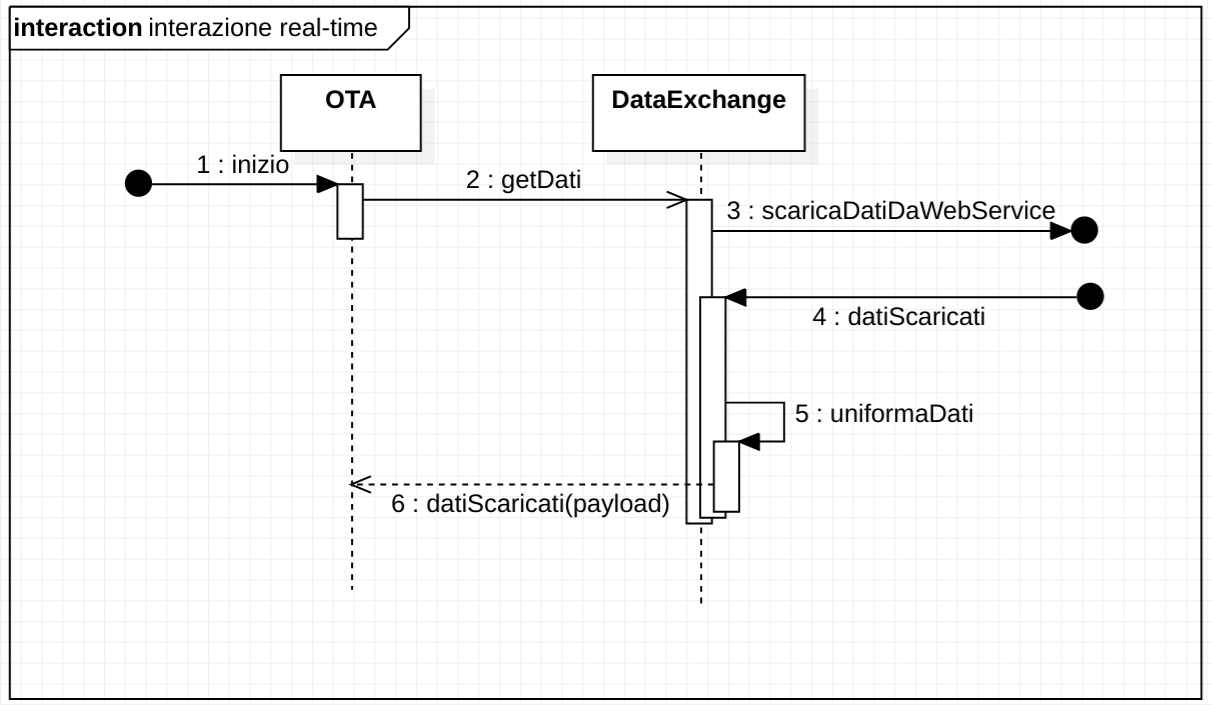
\includegraphics[width=.75\columnwidth]{attivita/interazione_realtime} 
		\caption{Schema dell'integrazione in tempo reale DataExchange-OTA.}
		\label{figura:integrazione-realtime}
	\end{figure}
\end{itemize}

\subsection{Flusso di prenotazione}
\label{section:flusso-prenotazione}
Quando il visitatore, in seguito alla ricerca, apre i dettagli di una partenza, viene data la possibilità di poter avviare la procedura (flusso) di prenotazione, che si avvale dell'interazione real-time tra \textit{OTA} e \textit{DataExchange} si compone nei seguenti punti:
\begin{enumerate}
	\item \textit{categoryAvailability}: vengono elencati i gruppi (categorie) di cabine effettivamente disponibili (o un messaggio di errore in caso non vi siano più posti prenotabili) tenendo conto del numero di passeggeri inseriti (banalmente, se si selezionano 4 passeggeri, vengono mostrati le categorie di cabine nelle quali vi è presente almeno una quadrupla) e dell'età di tali passeggeri (per il calcolo preciso della tariffa, in quanto un minore paga meno di un adulto);
	\item \textit{cabinAvailability}: una volta selezionato una categoria di cabine, vengono mostrate tutte le cabine (una per una) ancora disponibili, raggruppate in base al ponte della nave in cui si trovano;
	\item \textit{categoryItem}: vengono elencati tutti i servizi extra (e relativi prezzi) disponibili in aggiunta a quelli già inclusi nel prezzo della cabina, e viene data la possibilità di selezionarli per aggiungerli alla prenotazione;
	\item \textit{requestPricing}: viene mostrato il prezzo finale (preso dal \gls{webservice} del fornitore) della prenotazione, tenendo conto di quanto selezionato negli step precedenti. Tale prezzo include anche le tasse portuali ed eventuali oneri aggiuntivi;
	\item \textit{requestBooking}: viene effettuata una prenotazione od un'opzione di quanto selezionato negli step del flusso precedenti. Nel caso di prenotazione, viene anche gestito il pagamento (tramite \gls{api} fornite dal consorzio \textit{Triveneto Bassilichi}).
	\item \textit{requestBookingInformation}: viene mostrato il riepilogo di ciò acquistato, con la possibilità di saldare quanto ancora dovuto (nel caso la prenotazione ammetta il versamento di un acconto).
\end{enumerate}

\subsection{Struttura del codice}
\label{section:struttura-codice}
Sia \textit{OTA} che \textit{DataExchange} sono realizzati usando il \gls{framework} \textit{Codeigniter}. Questo implica che applicano a PHP il paradigma \textit{Object-oriented} (orientato agli oggetti) associato al design pattern \gls{mvc}. Entrambi i progetti, dunque, presentano tre tipologie di classi:
\begin{itemize}
	\item \textbf{Model}, che estendono la classe base \textit{CI\_Model}, i quali sono la chiave di accesso ai dati dell'applicazione. Si è deciso di realizzare un \textit{model} per ogni tabella presente nel database;
	\item \textbf{View}, che generano il codice HTML di ogni pagina (o porzione di essa). Alle \textit{view} é possibile passare delle variabili in modo da rendere dinamico il loro contenuto.
	\item \textbf{Controller}, che estendono la classe base \textit{CI\_Controller} e istanziano le \textit{view} popolandole con i dati provenienti dai \textit{model}. La particolarità di queste classi è che i loro metodi pubblici si possono chiamare direttamente tramite URL. Codeigniter, infatti, implementa un meccanismo (grazie al \textit{magic method \_\_call}) per il quale é possibile chiamare un metodo pubblico \textit{a} di una classe controller \textit{C} semplicemente recandosi all'url \textit{nomedelsito.dominio/C/a} (ad esempio \textit{crociereregalo.it/C/a}). Tale meccanismo risulta molto utile nella realizzazione di \gls{api} e nella creazione di \textit{URL} user-friendly (quindi più leggibili)
\end{itemize} 
Codeigniter, inoltre, presenta un modulo personalizzato per interagire con il database, che supporta funzionalità come il \textit{log delle query} (in pratica è possibile sapere l'ultima query eseguita, molto utile in caso di debug), meccanismi di \textit{query builder} (creazione assitita di query), \textit{query parametrizzate}, gestione delle transazioni ecc.

\section{Ottimizzazione delle performance del database}
\subsection{Il problema}
Il sito CrociereRegalo soffriva di un grande problema: la velocità di caricamento delle pagine. Tale lentezza era dovuta principalmente all'elevato numero di query complesse presenti in ogni pagina, ciascuna delle quali aveva dei tempi di esecuzione nell'ordine dei secondi che, complessivamente, facevano sì che il tempo di caricamento di alcune pagine (in primis quella di visualizzazione dei risultati di una ricerca) lambisse pericolosamente il minuto.
\subsection{La soluzione trovata}
Dopo un'attenta analisi del database, é emerso che molte tabelle non avevano una corretta struttura. In particolare, su alcune non vi era definita alcuna chiave primaria, mentre in generale non erano presenti chiavi esterne ed indici. Sono quindi state definite chiavi esterne e primarie per tutte le tabelle, mentre per la creazione di indici ci si è affidati all'analisi delle principali query grazie allo strumento \textit{Database Tuning Engine Advisor} integrato nella suite di \textit{SQL Server}. Vengono ora riportati due esempi di analisi svolta e di risultati ottenuti.
\subsubsection{Query di ricerca}

\begin{lstlisting}
SELECT distinct TOP 100 l.Supplier, l.NameIT, l.Description, l.Logo, il.ShipCode,il.SailingLengthDays, il.ItineraryCode, po1.Code as PortoPartenzaCode ,po1.Name as PortoPartenza, po2.Name as PortoArrivo, po2.Code as PortoArrivoCode, min(il.SailingDate) as MinSailingDate, min(p.BestPrice) as BestPrice,it.GraphicsUrl,sp.Name as ShipName 
FROM Cruises_ItineraryList il inner join Cruises_Lines l on il.Supplier= l.Supplier inner join Cruises_Ports po1 on (po1.Code = il.DepartingPort and po1.Supplier = il.Supplier ) inner join Cruises_Ports po2 on (po2.Code = il.EndPort and po2.Supplier = il.Supplier) inner join Cruises_Ship sp on (sp.Supplier=il.Supplier and sp.Code = il.ShipCode) inner join Cruises_Prices p on (p.Supplier=il.Supplier and p.CruiseId = il.CruiseID and p.CruiseCategoryAvailable=1) inner join Cruises_Itinerary it on (it.Supplier=il.Supplier and il.ItineraryCode = it.Code) 
WHERE il.Supplier=1 AND il.AvailabilityStatusCode= 'AV' AND BestPrice > 0 
GROUP By l.Supplier, l.NameIT, l.Description, l.Logo, il.ShipCode,il.SailingLengthDays, il.ItineraryCode, po1.Code, po2.Code, po1.Name, po2.Name , sp.ImgUrl,it.GraphicsUrl,sp.Name order by MinSailingDate,PortoArrivo,ItineraryCode
\end{lstlisting}
Questa é una delle query (la più esterna) che viene usata nel caso di ricerca di un itinerario filtrandolo per fornitore (in questo caso MSC Crociere). Il problema di questa interrogazione, oltre alla lunghezza, è l'elevato numero di JOIN tra tabelle aventi un ingente quantitativo di dati, nello specifico:
\begin{itemize}
	\item Cruises\_Prices: 424 780 righe
	\item Cruises\_ItineraryList: 8 092 righe
	\item Cruises\_Ports: 4 187 righe
	\item Cruises\_Itinerary: 2 985 righe
\end{itemize}

Tali tabelle erano per lo più sprovviste di indici, pertanto le operazioni di JOIN risultavano molto costose. Come risultato si otteneva un tempo di esecuzione, nel server di produzione in assenza di sovraccarichi, variabile tra 23 e 25 secondi. Grazie al tool \textit{Database Tuning Engine Advisor} sono stati creati dei nuovi indici, precisamente su tutte le colonne coinvolte nelle clausole di JOIN. Questo ha portato un ingente riduzione nei tempi di esecuzione della query, che sono arrivati a sfiorare i 2 secondi. Vi è stato, quindi, un miglioramento di ben almeno 21 secondi (circa il 91\%) nel tempo di esecuzione della query e di conseguenza nel \gls{tempodirisposta} della pagina web incaricata di elaborare e visualizzare i risultati della ricerca.\\
\begin{figure}[!h] 
	\centering 
	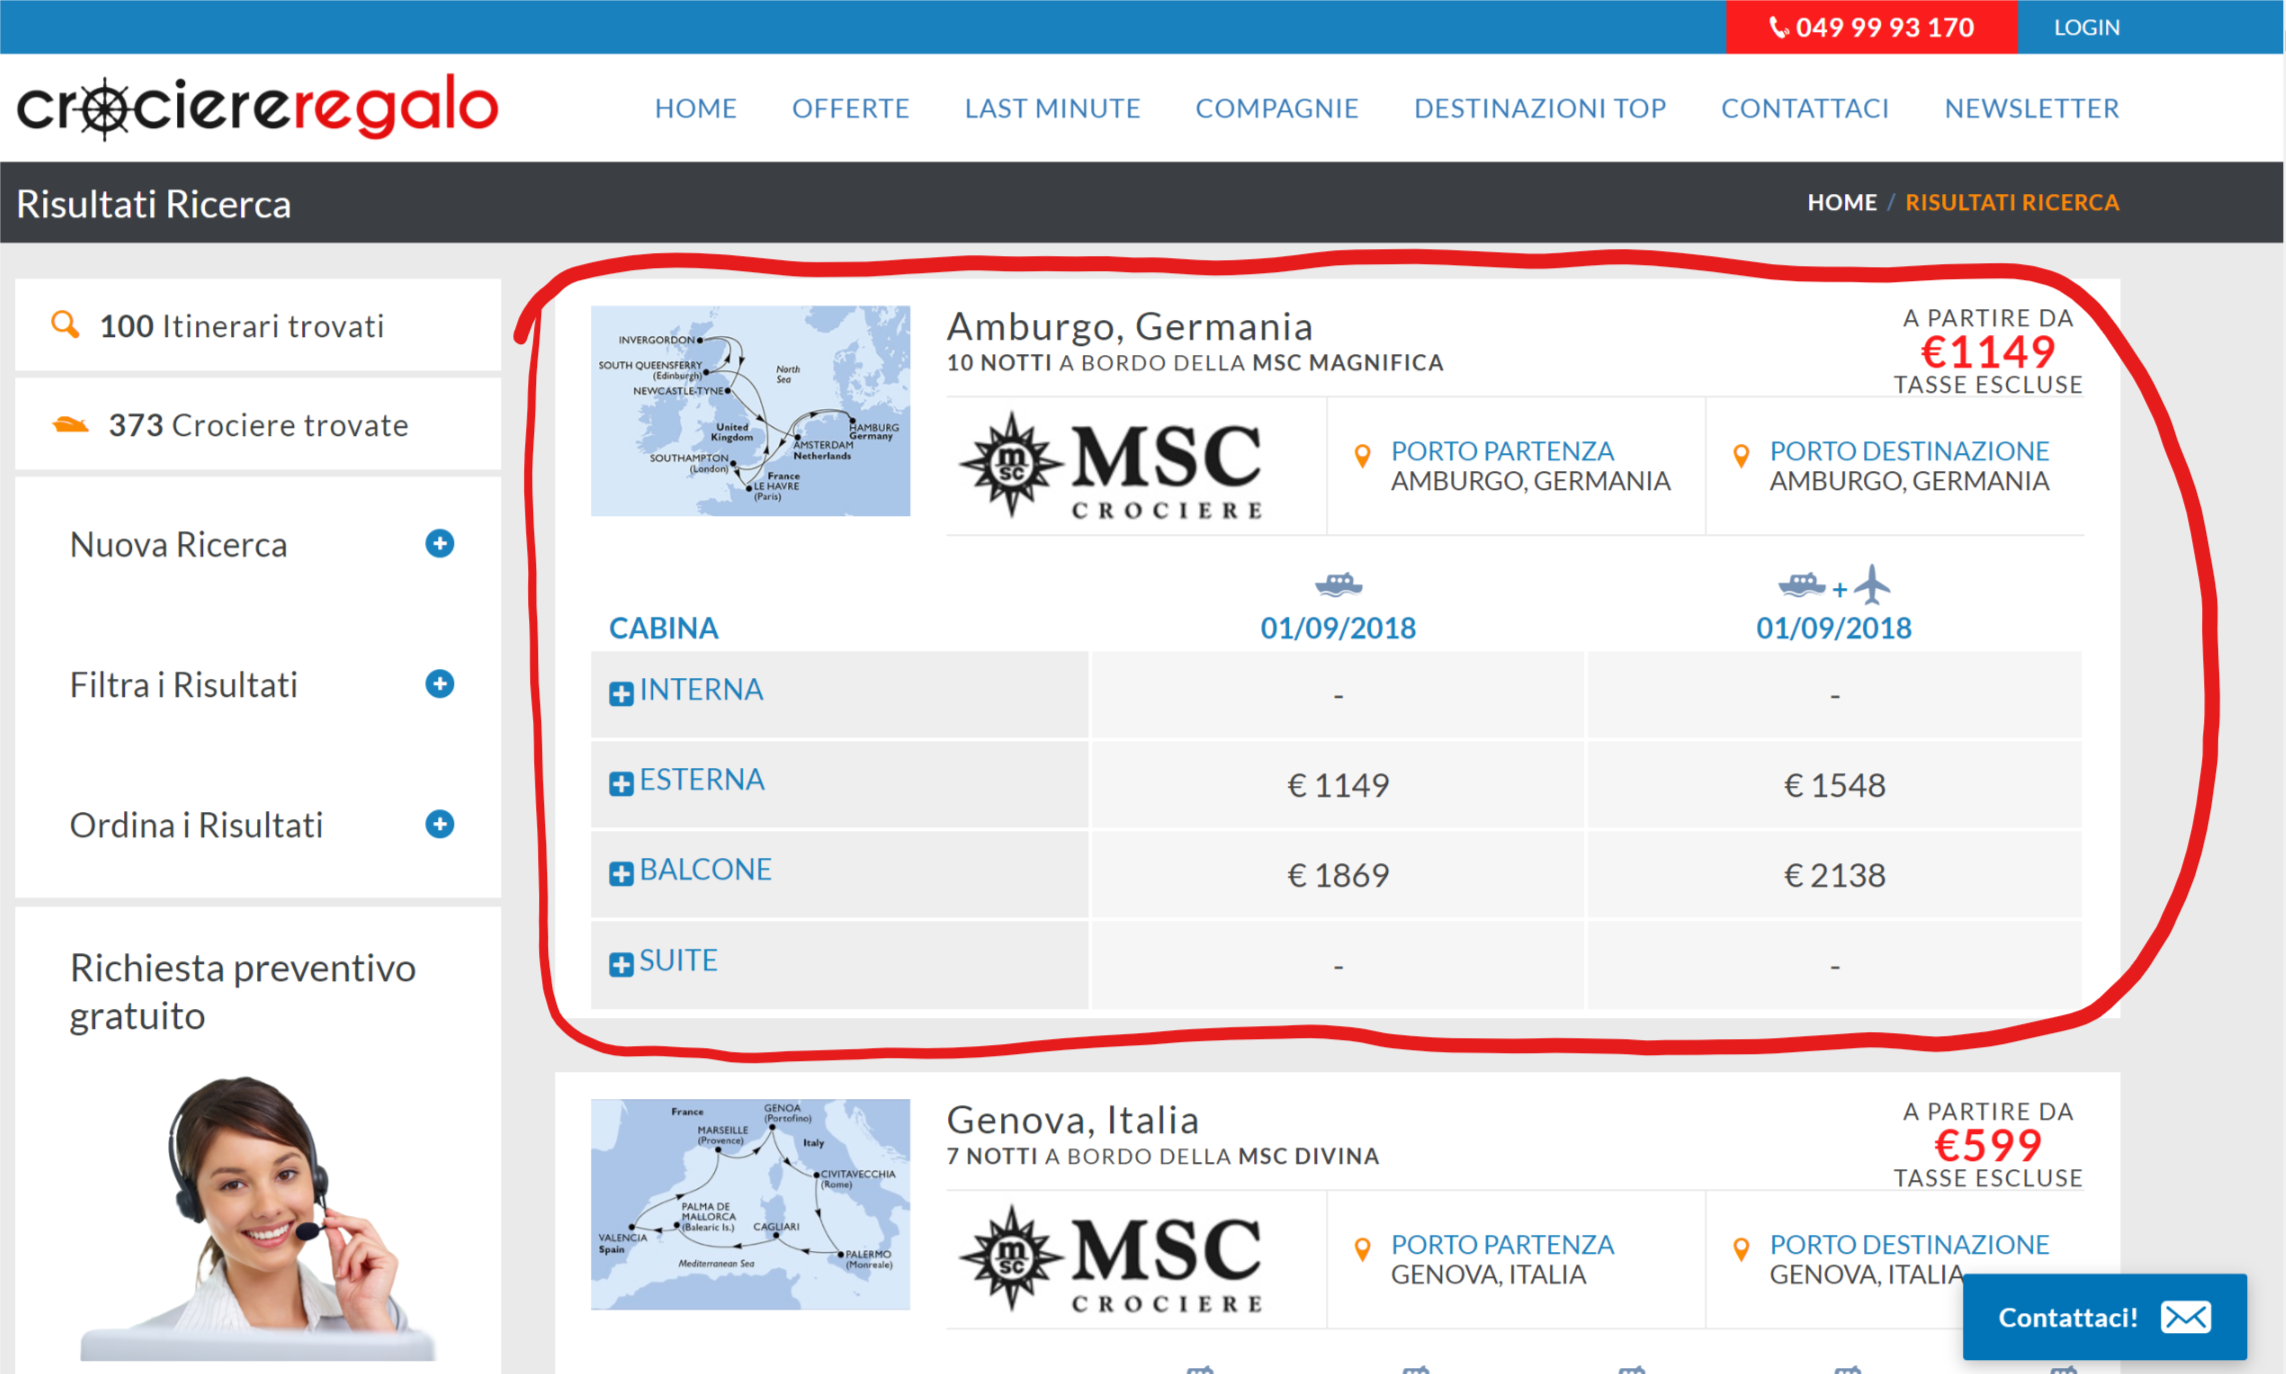
\includegraphics[width=1\columnwidth]{attivita/risultato_ricerca} 
	\caption{Esempio di utilizzo del risultato della query sopra menzionata.}
\end{figure}

\subsubsection{Query dei last minute}
In homepage vi è una sezione che visualizza tutte le offerte \textit{last minute} (ovvero crociere prossime alla partenza aventi ancora posti disponibili a prezzo scontato) presenti nel database. Queste ultime vengono inserite a mano dai dipendenti di \textit{Primarete}, ma sono collegate a crociere effettivamente presenti. La query sottostante restituisce tali offerte.
\begin{lstlisting}
SELECT distinct top 4 l.Logo,l.NameIT as SupplierName,il.Supplier,il.CruiseID,il.ShipCode, il.ItineraryCode,il.DepartingPort,il.EndPort,il.SailingDate,il.ReturnDate,il.SailingLengthDays as NightNumber,po.Name as Partenza,po2.Name as Arrivo,s.foto,sp.ImgUrl,min(p.BestPrice) as BestPrice FROM Cruises_ItineraryList il join Cruises_Prices p on il.CruiseID = p.CruiseId join Cruises_Ports po on (il.DepartingPort = po.Code and po.Supplier=il.supplier) join Cruises_Ports po2 on (il.EndPort = po2.Code and po2.Supplier=il.supplier) join Cruises_Ship sp on (sp.Code=il.ShipCode and sp.Supplier=il.Supplier) join Cruises_Lines l on (l.Supplier=il.Supplier) left join Cruises_Banner AS b ON b.tipo = 'nave' AND b.riferimento = CONCAT(il.Supplier,'-',il.ShipCode) INNER JOIN Cruises_Banner_Slide AS s ON b.id = s.banner AND s.nome='nave'
 WHERE SailingDate BETWEEN '2018-09-09' and '2018-10-09' and AvailabilityStatusCode='AV' and il.supplier = 2 and po.Supplier= 2 and po2.Supplier=2 and p.BestPrice>0 group by l.Logo,l.NameIT,il.Supplier,il.CruiseID,il.ShipCode, il.ItineraryCode,il.DepartingPort,il.EndPort,il.SailingDate,il.ReturnDate,il.SailingLengthDays,po.Name ,po2.Name ,s.foto,sp.ImgUrl
\end{lstlisting}
Anche qua, il numero di JOIN su tabelle aventi ingenti quantità di dati rende il tempo di esecuzione della query molto elevato in caso il database non sia sufficientemente ottimizzato. Grazie alle ottimizzazioni suggerite dal tool \textit{Database Tuning Engine Advisor}, si è avuto un miglioramento del tempo di esecuzione indicativamente dell'83\%, che è passato da 3 secondi a 0.5. Tale miglioramento si è riflettuto anche nelle performance della homepage, che ha visto una netta diminuzione del tempo medio di risposta.
\begin{figure}[!h] 
	\centering 
	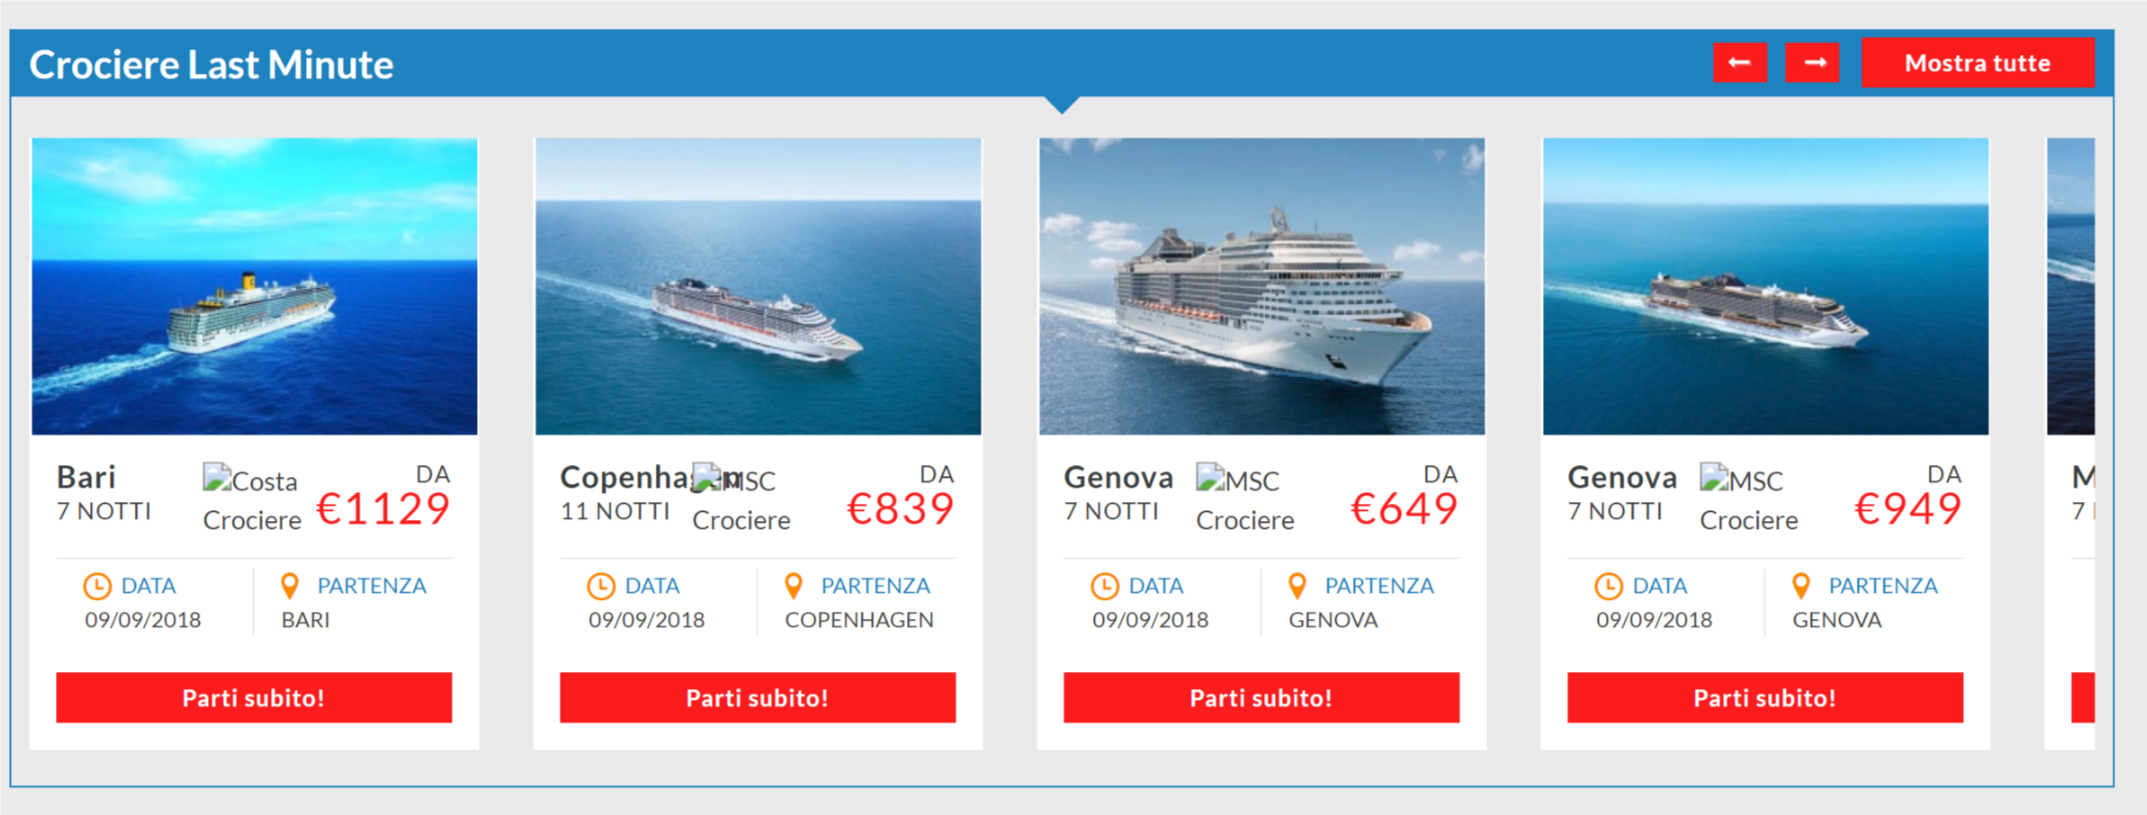
\includegraphics[width=1\columnwidth]{attivita/last_minute} 
	\caption{Esempio di utilizzo del risultato della query sopra menzionata.}
\end{figure}

\subsection{Conclusioni}
Al termine delle ottimizzazioni, sono stati ottenuti buoni risultati (il \gls{tempodirisposta} del sito è diminuito di almeno il 50\%), ma non abbastanza per rendere il sito reattivo ed equiparabile in termini di velocità ai competitor. Si è deciso quindi di esplorare nuove soluzioni.

\section{Cache delle query}
\subsection{Il problema}
Se é vero che, al termine degli interventi sulla struttura del database descritti nella sezione precedente, le prestazioni delle interrogazioni erano migliorate molto, è anche vero che il sito non aveva raggiunto livelli di prestazioni ottimali. Infatti alcune pagine avevano ancora un \gls{tempodirisposta} molto elevato. Prendendo come esempio la pagina del sito più utilizzata, ovvero quella di visualizzazione dei risultati di una ricerca, essa è passata da un \gls{tempodirisposta} tra i 45 e i 60 secondi ad un \gls{tempodirisposta} tra i 15 e i 20 secondi, comunque troppo per le aspettative di un internauta medio: basti pensare che il principale competitor (\url{www.logitravel.it}) ha un \gls{tempodirisposta} che si attesta attorno al secondo e mezzo (10 volte meno) per la stessa funzionalità.

\subsection{La soluzione}
La soluzione trovata a tale problema nasce dalla seguente considerazione: é possibile prevedere quando cambia la maggior parte dei dati presenti nel database e utilizzati per le query più lente. Infatti dati inerenti a navi, itinerari, cabine, prezzi e disponibilità vengono rinnovati ad ogni integrazione, che è un'operazione schedulata 4 volte al giorno, ad orari noti. Osservando inoltre che la stessa query sugli stessi dati presenta gli stessi risultati, si è giunti alla conclusione che l'implementazione di un meccanismo di caching delle query permetta di ottimizzare velocità del sito e carico del server.\\
Il meccanismo progettato ha il seguente funzionamento:
\begin{itemize}
	\item La query viene eseguita la prima volta ed il suo risultato viene salvato nella cache;
	\item Quando la query viene eseguita ancora, invece di interrogare il database viene letto il contenuto della cache;
	\item Ad ogni integrazione dati la cache viene svuotata, perchè i dati presenti in essa non riflettono più il nuovo contenuto delle tabelle del database;
	\item Al termine di ogni integrazione, vengono effettuate delle richieste \textit{CURL} alle pagine più utilizzate del sito, in modo tale che la cache venga ricreata.
\end{itemize}
Si è deciso di affidare la gestione della cache a \textit{Codeigniter}, che offre già questa funzionalità. Il modulo di gestione del database di \textit{Codeigniter}, infatti, fornisce già i seguenti metodi:
\begin{itemize}
	\item \textit{cache\_on}, che permette di abilitare la cache;
	\item \textit{cache\_off}, che permette di disabilitare la cache;
	\item \textit{cache\_delete}, che permette di cancellare la cache di una singola pagina (passata come parametro);
	\item \textit{cache\_delete\_all}, che permette di cancellare tutto il contenuto della cache.
\end{itemize}
Combinando l'uso di \textit{cache\_on} e \textit{cache\_off}, si può anche disabilitare la cache per determinate query, che magari operano su dati più "volatili" e aventi minor quantità. \\In generale, comunque, \textit{Codeigniter} salva i risultati delle varie query in dei file di cache (aventi come nome l'hash della query a cui tale file si riferisce) suddivisi per cartelle in base all'url che le ha generate.
\begin{figure}[!h] 
	\centering 
	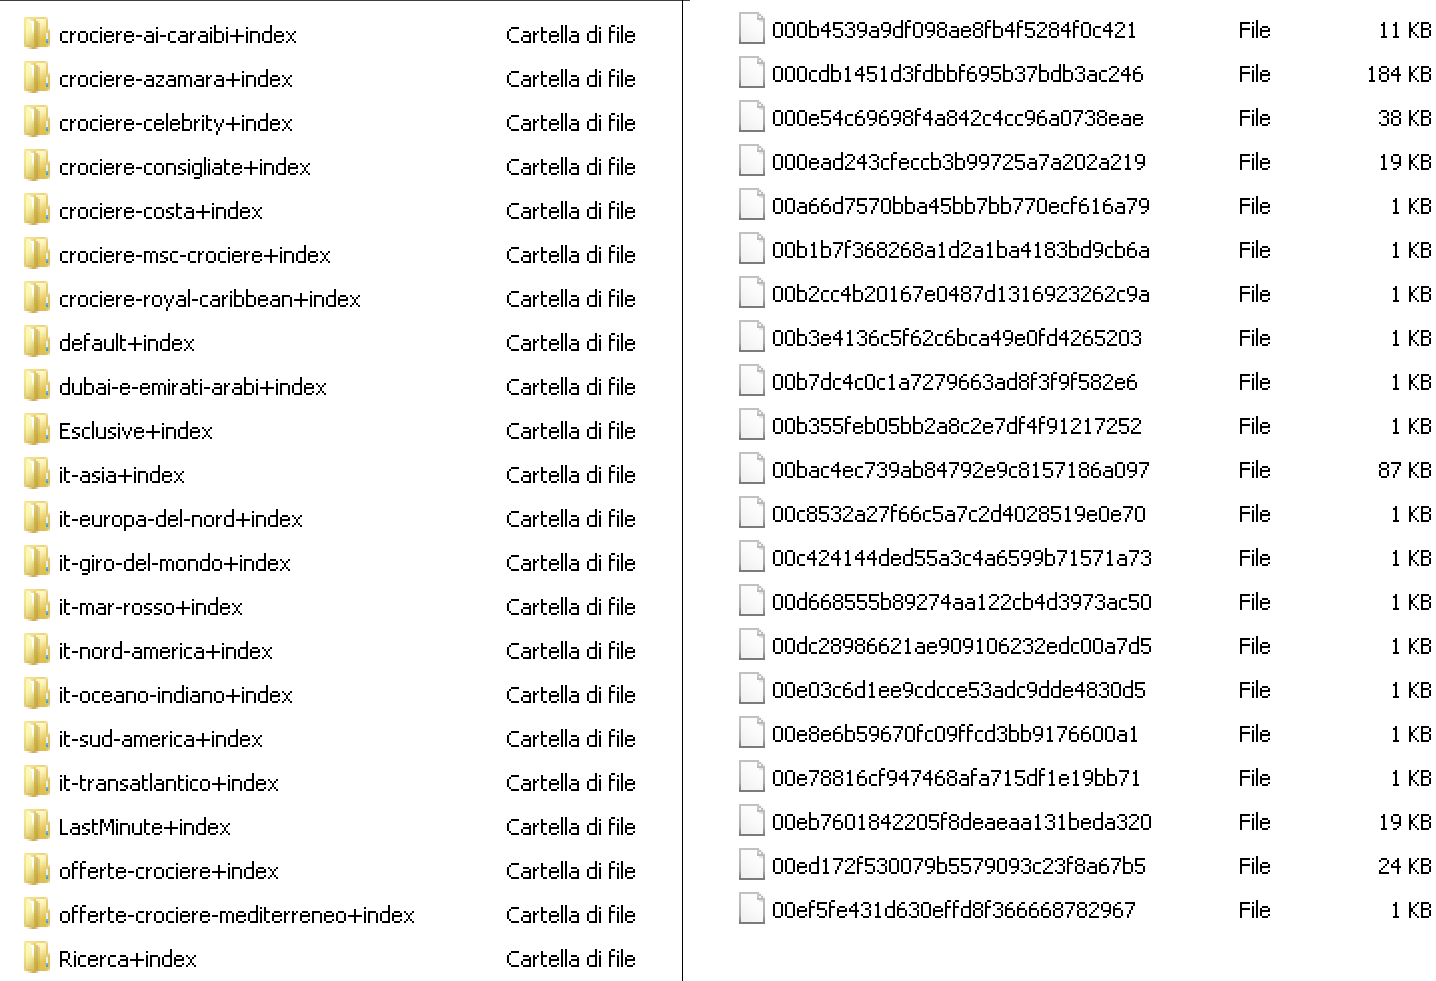
\includegraphics[width=1\columnwidth]{attivita/cache_codeigniter} 
	\caption{Struttura di cartelle e file di cache in esse contenuti.}
\end{figure}
Grazie a \textit{cache\_delete} sarebbe possibile cancellare la cache solo di alcune pagine, ma è stato preferito non utilizzare tale funzione in quanto avrebbe aumentato inutilmente la complessità della soluzione.

\subsection{Risultati}
L'implementazione della cache ha giovato molto al \bookingEngine. Basti pensare che ora la pagina di visualizzazione dei risultati ricerca è giunta ad avere un tempo di risposta medio attorno ai 3 secondi, ovvero ora è l'80\% più veloce di prima, ma soprattutto è paragonabile al tempo di risposta dei competitor. Il tempo di risposta della homepage, inoltre, è arrivata a toccare i 500 millisecondi, dai circa 3 secondi prima di implementare la cache.\\
Tra ottimizzazione del database e cache, comunque, sono stati fatti ingenti miglioramenti alle prestazioni, che riassumo nella tabella sottostante, prendendo come esempio la pagina principale e quella di visualizzazione dei risultati della ricerca (che, per brevità, chiamerò soltanto "ricerca").\\

\begin{center}
	\def\arraystretch{1.5}
	\begin{tabular}{ | l | l | l | l |}
		\hline
		\textbf{Pagina} & \textbf{Senza ottimizzazioni} & \textbf{Con DB ottimizzato} & \textbf{Con cache} \\ \hline
		Homepage & 7 secondi & 3 secondi & 0.5 secondi.  \\
		\hline
		Ricerca & 45-60 secondi & 15-20 secondi & 3 secondi.  \\
		\hline
	\end{tabular}
\end{center}

\newpage
\section{Integrazione delle tariffe vuoto per pieno}
\subsection{Il problema}
Dopo aver preso effettivamente confidenza con il database, mi è stato chiesto come secondo lavoro di creare un sistema che permettesse di inserire nel flusso di prenotazione anche tariffe vuoto per pieno. Precisamente, tale sistema avrebbe dovuto avere le seguenti caratteristiche:
\begin{enumerate}
	\item Permettere di inserire nel sistema gli acquisti di vuoti pieno effettuati da \textit{Primarete} tramite upload di appositi file;
	\item Permettere di differenziare i prezzi in base al soggetto a cui si sta vendendo;
	\item Permettere di prenotare e pagare una cabina con tariffa vuoto per pieno.
\end{enumerate}

\subsubsection{Inserimento degli acquisti nel sistema}
Il sistema avrebbe dovuto prevedere una funzionalità di "carico" delle tariffe. In fase di acquisto dei vuoti pieno da parte di \textit{Primarete}, il fornitore (ovvero la compagnia di crociera) rilascia un file riepilogativo contenente il dettaglio di quanto acquistato. Tali informazioni avrebbero dovuto potersi caricare in modo assistito nel sistema, che avrebbe dovuto poi inserirle nel flusso di prenotazione.\\
Il problema principale è stato che il file ritornato da ciascun fornitore aveva (e ha tuttora) il proprio formato dati, quindi si sarebbe dovuto creare un importatore per ogni fornitore. Inoltre, anche la tipologia di dati presente in ciascun file poteva differire: ad esempio, per riferirsi all'età di ogni passeggero, alcuni fornitori utilizzano l'età ed altri la data di nascita. Il sistema avrebbe dunque dovuto uniformare i dati caricati.

\subsubsection{Differenziazione dei prezzi}
CrociereRegalo è un \bookingEngine\hphantom{i}utilizzato per vendite sia B2C (cioè verso clienti finali) sia B2B (cioè verso altre agenzie). Queste ultime, in base agli accordi commerciali che hanno con \textit{Primarete}, appartengono a determinati \textit{listini}, ovvero hanno diritto a commissioni/tariffe più o meno agevolate.\\Il sistema, quindi, avrebbe dovuto poter differenziare i prezzi di vendita delle cabine in base al listino di appartenenza dell'acquirente (un acquirente non appartenente a nessun listino sarebbe stato identificato al pari di una vendita B2C).

\subsubsection{Inserimento della tariffa nel flusso di prenotazione}
Il \bookingEngine\hphantom{i}avrebbe dovuto permettere di visualizzare i prezzi delle cabine soggette a tariffe vuoto per pieno nei risultati di ricerca. Inoltre, avrebbe dovuto essere possibile poter prenotare e conseguentemente pagare tali cabine.\\La disponibilità delle stesse, quindi, si sarebbe dovuta aggiornare (decrementare) automaticamente.

\subsection{La soluzione}
\subsubsection{Inserimento degli acquisti nel sistema}
Affinché fosse possibile inserire gli acquisti nel sistema, è stata realizzata una nuova pagina nel pannello di amministrazione del \bookingEngine, accessibile solo tramite l'inserimento di username e password. In tale pagina viene visualizzato un riepilogo dei vuoti pieno caricati con la possibilità, per ognuno di essi, di avere il dettaglio delle cabine vendute e di quelle ancora disponibili. È stato inoltre inserito un tasto che apre una finestra di dialogo all'interno della quale viene data la possibilità di caricare nuovi vuoti pieno, andando quindi a "rifornire" il "magazzino". In base al fornitore selezionato nella finestra di dialogo è possibile: 
\begin{itemize}
	\item Caricare il file di riepilogo di quanto acquistato fornito dalla compagnia, in caso di fornitore \textbf{Costa} o \textbf{MSC}. Il primo fornisce un file con estensione \textit{.xls} mentre il secondo un file con estensione \textit{.csv}
	\begin{figure}[!h] 
		\centering 
		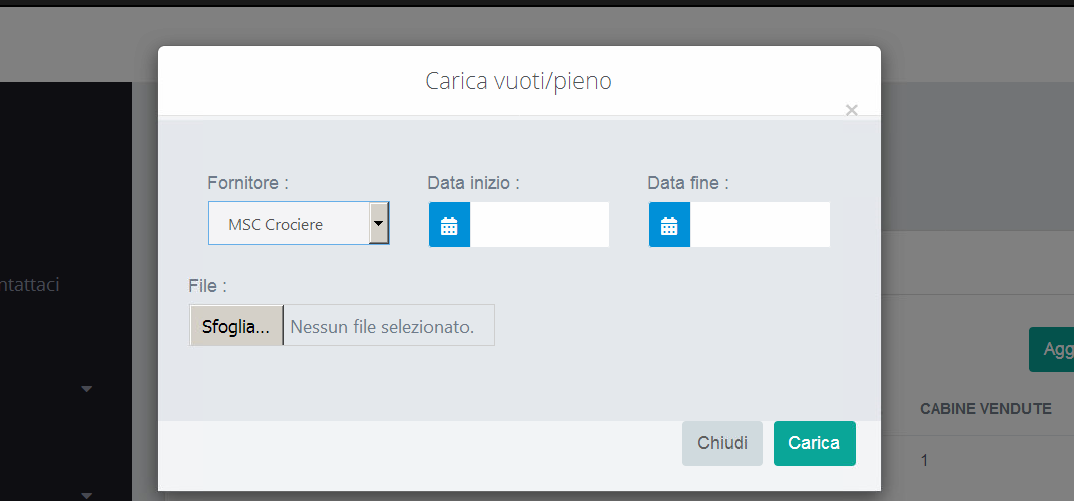
\includegraphics[width=.8\columnwidth]{attivita/vuotopieno_msc} 
		\caption{Schermata di caricamento del vuoto pieno MSC e Costa.}
	\end{figure}
	\item Inserire a mano i dettagli del vuoto pieno che si intende caricare nel caso di fornitore \textbf{Royal Caribbean}, \textbf{Celebrity} o \textbf{Azamara}. Essi infatti forniscono il file di riepilogo di quanto acquistato in formato \textit{.pdf}, che è molto difficile da interpretare.
	\begin{figure}[!h] 
		\centering 
		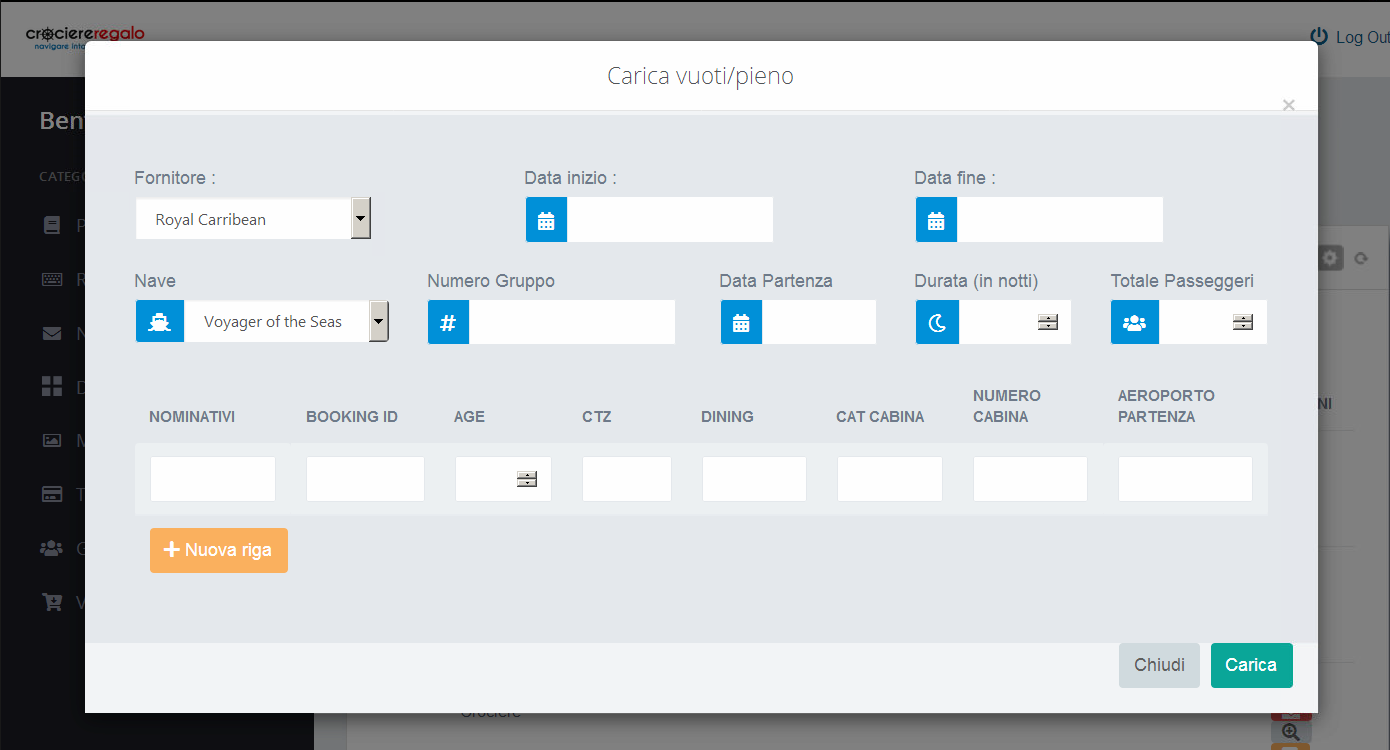
\includegraphics[width=.8\columnwidth]{attivita/vuotopieno_royal} 
		\caption{Schermata di caricamento del vuoto pieno Royal/Celebrity/Azamara.}
	\end{figure}
\end{itemize}
In ogni caso, é stato deciso che per ciascun vuoto pieno si sarebbero memorizzate le seguenti informazioni:
\begin{itemize}
	\item Il \textbf{fornitore}, ovvero MSC, Costa, Royal Caribbean, Celebrity o Azamara;
	\item Il \textbf{groupID}, ovvero un identificatore univoco per ciascun fornitore del vuoto pieno acquistato;
	\item Il \textbf{cruiseID}, ovvero un identificatore univoco per ciascun fornitore della crociera a cui tale vuoto pieno si riferisce;
	\item La \textbf{data di partenza} della crociera;
	\item La \textbf{lunghezza} (in numero di notti) della crociera;
	\item Il \textbf{numero di posti} (ovvero la capienza massima di persone) totali in quel vuoto pieno;
	\item Il \textbf{numero di cabine} totali di quel vuoto pieno,
	\item La \textbf{data di inizio} e la \textbf{data di fine} validità della tariffa, in modo che sia possibile venderla solo in determinati periodi/intervalli. Ciò significa che, ad esempio, se la data di inizio viene impostata al 20 agosto 2018 e la data di fine al 30 settembre 2018, in caso di una ricerca fatta prima del 20 agosto 2018 o dopo il 30 settembre 2018, la tariffa non comparirà tra i risultati.
\end{itemize}
Per memorizzare queste informazioni è stata creata una nuova tabella in database denominata \textbf{Cruises\_Inventory}, avente come campi \textit{Id} (chiave primaria auto incrementante), \textit{Supplier} (fornitore, chiave esterna che si riferisce a \textit{Cruises\_Lines}, tabella dove sono memorizzati tutti i fornitori), \textit{GroupID}, \textit{CruiseID}, \textit{DepartureDate} (data di partenza della crociera), \textit{Length} (lunghezza in notti della crociera), \textit{N\_Pax} (numero di posti totali), \textit{N\_Cab} (numero di cabine totali), \textit{Data\_Inizio} e \textit{Data\_Fine}.\\
\\
Oltre alle informazioni generali relative a ciascun vuoto pieno, è stato necessario memorizzarne anche il contenuto in dettaglio, in termini di cabine acquistate (e quindi da rivendere). Si è deciso di creare la tabella \textbf{Cruises\_InventoryDetail} avente i seguenti campi:
\begin{itemize}
	\item \textbf{Id}, chiave primaria auto incrementante;
	\item \textbf{Cruises\_Inventory}, chiave esterna collegata all'\textit{Id} dell'omonima tabella \textit{Cruises\_Inventory}, che serve per collegare ogni riga del dettaglio al vuoto pieno corrispondente;
	\item \textbf{Cruises\_PricesID}, chiave esterna collegata all'\textit{Id} di \textit{Cruises\_Prices}, tabella il cui scopo verrà analizzato nel dettaglio nella sezione successiva;
	\item \textbf{Cabin}, numero di cabina (univoco nel dominio del fornitore) a cui la riga corrente si sta riferendo;
	\item \textbf{BookId}, numero di prenotazione del fornitore della cabina a cui la riga corrente si sta riferendo;
	\item \textbf{Category}, categoria della cabina corrente.
\end{itemize}
Per gestire il caricamento dei vuoti pieno nel sistema sono state realizzate tre classi \textit{parser} (una per MSC, una per Costa e una per il trio Royal-Celebrity-Azamara)in grado di interpretare dei dati in input e renderli compatibili con la struttura delle tabelle \textit{Cruises\_Inventory} e \textit{Cruises\_InventoryDetail}. Queste tre classi, \textit{MSCParser}, \textit{CostaParser} e \textit{RoyalParser} implementano tutte l'interfaccia \textbf{ParserInterface}, che ha i seguenti metodi astratti:
\begin{center}
	\def\arraystretch{1.5}
	\begin{tabularx}{\columnwidth}{XX}
		\hline
		\textbf{Metodo} & \textbf{Descrizione} \\ \hline
		+ getCruiseID() : string & Ritorna il CruiseID corrispondente al vuoto pieno considerato\\
		\hline
		+ getGroupID() : string & Ritorna il GroupID corrispondente al vuoto pieno considerato\\
		\hline
		+ getDepartureDate() : string & Ritorna la data di partenza corrispondente al vuoto pieno considerato, in formato "Y-m-d" (esempio 2018-09-27).\\
		\hline
		+ getLength() : int & Ritorna la lunghezza (in numero di notti) corrispondente al vuoto pieno considerato.\\
		\hline
		+ getNPax() : int & Ritorna la capienza totale (in numero di persone) corrispondente al vuoto pieno considerato.\\
		\hline
		+ getNCab() : int & Ritorna la capienza totale (in numero di cabine) corrispondente al vuoto pieno considerato.\\
		\hline
		+ popolaDettaglioTabella() : array & Ritorna un array che, per ciascuna riga del vuoto pieno, associa a ciascun campo della tabella \textit{Cruises\_InventoryDetail} il relativo valore.\\
		\hline
	\end{tabularx}
\end{center}
È stata poi creata una nuova classe, \textbf{Cruises\_Inventory}, "figlia" di \textit{CI\_Model} (classe base dei modelli di Codeigniter), che si occupa principalmente del caricamento del vuoto pieno nel database, avvalendosi dei parser prima elencati. Di preciso, ha i seguenti metodi:
\begin{center}
	\def\arraystretch{1.5}
	\begin{longtable}{ >{\raggedright}p{5.5cm} p{6.8cm}} 
		\hline
		\textbf{Metodo} & \textbf{Descrizione} \\ \hline
		+ validId(id:int) : boolean & Ritorna \textit{true} se il parametro passato è un valore presente nella colonna "Id" della tabella \textit{Cruises\_Inventory}\\
		\hline
		+ loadFromFile (supplier: int, fileContent: string, dataInizio: Date, dataFine: Date) : void & In base al fornitore passato come parametro (\textit{supplier}), carica il contenuto del vuoto pieno (presente in \textit{fileContent}) nel database, avvalendosi del parser associato al fornitore.\\
		\hline
		- loadRoyalInput (supplier: int, content: array) : boolean & Carica il vuoto pieno Royal/Celebrity/Azamara (in base al valore della variabile \textit{supplier}) leggendo il contenuto dall'array associativo \textit{content} ed elaborandolo grazie al parser \textit{RoyalParser}.\\
		\hline
		- loadCostaFile (fileContent: string) : boolean & Carica il vuoto pieno Costa nel database; \textit{fileContent} rappresenta il contenuto del file del vuoto pieno caricato, che verrà elaborato dal parser \textit{CostaParser}.\\
		\hline
		- loadMSCFile (fileContent: string) : boolean & Carica il vuoto pieno MSC nel database; \textit{fileContent} rappresenta il contenuto del file del vuoto pieno caricato, che verrà elaborato dal parser \textit{MSCParser}.\\
		\hline
		- saveParsedFile(parser: ParserInterface, supplier: int) : boolean & Metodo che viene chiamato da \textit{loadRoyalInput}, \textit{loadCostaFile}, \textit{loadMSCFile}; serve a popolare la tabella \textit{Cruises\_InventoryDetail} e la tabella \textit{Cruises\_Prices}.\\
		\hline
	\end{longtable}
\end{center}
La gestione del pannello di amministrazione è affidata ad un unico \textit{controller}, chiamato \textbf{Back}. In questa classe è stato aggiunto un metodo chiamato \textit{caricaVuotoPieno} che prende l'input dal frontend e lo passa al metodo \textit{loadFromFile} della classe \textit{Cruises\_Inventory} appena descritta, che si occuperà dell'elaborazione e della restituzione del risultato della stessa sotto forma di \gls{json}.

\subsubsection{Differenziazione dei prezzi}
I prezzi di ogni cabina presente nel sistema risiedono nella tabella \textit{Cruises\_Prices}. Tale tabella permette di conoscere il prezzo di ogni categoria di cabina (per ogni combinazione di età dei passeggeri tollerata dal sistema) per ogni \gls{tariffa} disponibile. Il problema è che \textit{Cruises\_Prices} viene svuotata e ripopolata ad ogni integrazione: per questo motivo si è deciso di separare la gestione dei prezzi delle cabine soggette a tariffa vuoto per pieno in una nuova tabella, che è stata chiamata \textit{Cruises\_InventoryPrices}. Di preciso:
\begin{itemize}
	\item Nella tabella \textit{Cruises\_Prices} è stata inserita una nuova colonna di tipo intero, \textbf{Manuale}, che indica se la riga si sta riferendo ad una tariffa passata dal fornitore o presa da un vuoto pieno. Quando viene fatta un'integrazione, vengono eliminate solo le righe aventi valore di tale colonna pari a 0, in modo da non perdere le informazioni relative al vuoto pieno;
	\item È stata creata la tabella \textbf{Cruises\_InventoryPrices}, avente i seguenti campi:
		\begin{itemize}
			\item \textit{Id}, identificatore univoco della riga;
			\item \textit{Cruises\_Inventory}, chiave esterna che si riferisce al campo \textit{Id} di \textit{Cruises\_Inventory} e specifica il vuoto pieno di appartenenza di tale riga;
			\item \textit{Listino}, chiave esterna di \textit{Cruises\_Listini}, tabella appena creata che verrà descrittà nel prossimo paragrafo. In caso di valori NULL, il listino si intende essere \textit{B2C}, ovvero vendita al dettaglio;
			\item \textit{Categoria}, che rappresenta la categoria della cabina a cui ci si sta riferendo;
			\item \textit{Cabina}, che rappresenta il numero di cabina a cui ci si sta riferendo;
			\item \textit{BookId}, che indica il codice di prenotazione del fornitore collegato alla cabina a cui ci si sta riferendo;
			\item Un campo per ogni combinazione di prezzi tollerata dal sistema, ovvero \textit{Price1Adult, Price2Adult, Price3Adult, Price4Adult, Price1Adult1Junior, Price1Adult1Junior1Child, Price2Adult1Child, Price2Adult2Child,Price2Adult1Child, Price2Adult2Junior, Price2Adult1Junior1Child};
			\item \textit{Commissione}, che quantifica la commissione spettante all'agenzia viaggi collegata al listino specificato, in caso il campo \textit{Listino} non sia NULL.
		\end{itemize}
\end{itemize}
La tabella \textbf{Cruises\_Listini} menzionata precedentemente è stata creata per poter gestire tutti i listini da collegare alle varie agenzie viaggi. Tale tabella presenta due campi, \textit{Id} e \textit{Nome}, usati appunto per definire il listino stesso. \\
Nella tabella \textit{Cruises\_Utenti}, che raccoglie tutte le agenzie viaggio che possono accedere alla modalità di acquisto B2B, è stato aggiunto il campo \textit{Listino}, chiave esterna di \textit{Cruises\_Listini}, in modo da associare ogni agenzia registrata ad un listino, in base agli accordi presi con \textit{Primarete}. \\ \\
Per l'interazione con la tabella \textit{Cruises\_InventoryPrices} è stato creato un nuovo model avente lo stesso nome della tabella, con i seguenti metodi: 
\begin{center}
	\def\arraystretch{1.5}
	\begin{longtable}{ >{\raggedright}p{5.5cm} p{6.8cm}} 
		\hline
		\textbf{Metodo} & \textbf{Descrizione} \\ \hline
		+ getColonnePrezzi() : array & Ritorna un array contentente la lista di tutte le combinazioni di prezzi tollerata dal sistema. Questo metodo è stato scritto per rendere poi dinamico l'inserimento dei prezzi in questa tabella, ovvero in caso si voglia aggiungere un nuovo campo non presente (ad esempio \textit{Price6Adult}), sarà sufficiente aggiungerlo come colonna della tabella, e interfaccia grafica e query di inserimento si adatteranno automaticamente. \\
		\hline
		+ tentaAggiornamentoPrezzi (tabella: array, inventoryId: int) : void & Metodo che prova ad aggiornare i prezzi nel caso di caricamento di un vuoto pieno contenente cabine già presenti nel sistema.\\
		\hline
		+ salvaPrezzi (input: array) : boolean & Metodo che salva i prezzi di ogni cabina, per ogni listino, presenti nel parametro \textit{input}. Ritorna \textit{true} in caso di successo, \textit{false} altrimenti.\\
		\hline
		+ modificaPrezzi (input: array) : boolean & Metodo che modifica i prezzi di ogni cabina, per ogni listino, presenti nel parametro \textit{input}. Ritorna \textit{true} in caso di successo, \textit{false} altrimenti.\\
		\hline
	\end{longtable}
\end{center}
È stato inoltre creato un metodo \textit{salvaPrezzi} nel controller \textit{Back}, che si limita ad invocare il metodo \textit{salvaPrezzi} del model \textit{Cruises\_InventoryPrices} con i parametri passati tramite POST.\\
A livello frontend, si è fatto in modo che, al termine del caricamento del vuoto pieno, si venga reindirizzati ad una pagina di inserimento prezzi, che permette appunto di specificare ogni combinazione di prezzo tollerata dal sistema per ogni categoria di cabina per ciascun listino. 
	\begin{figure}[!h] 
	\centering 
	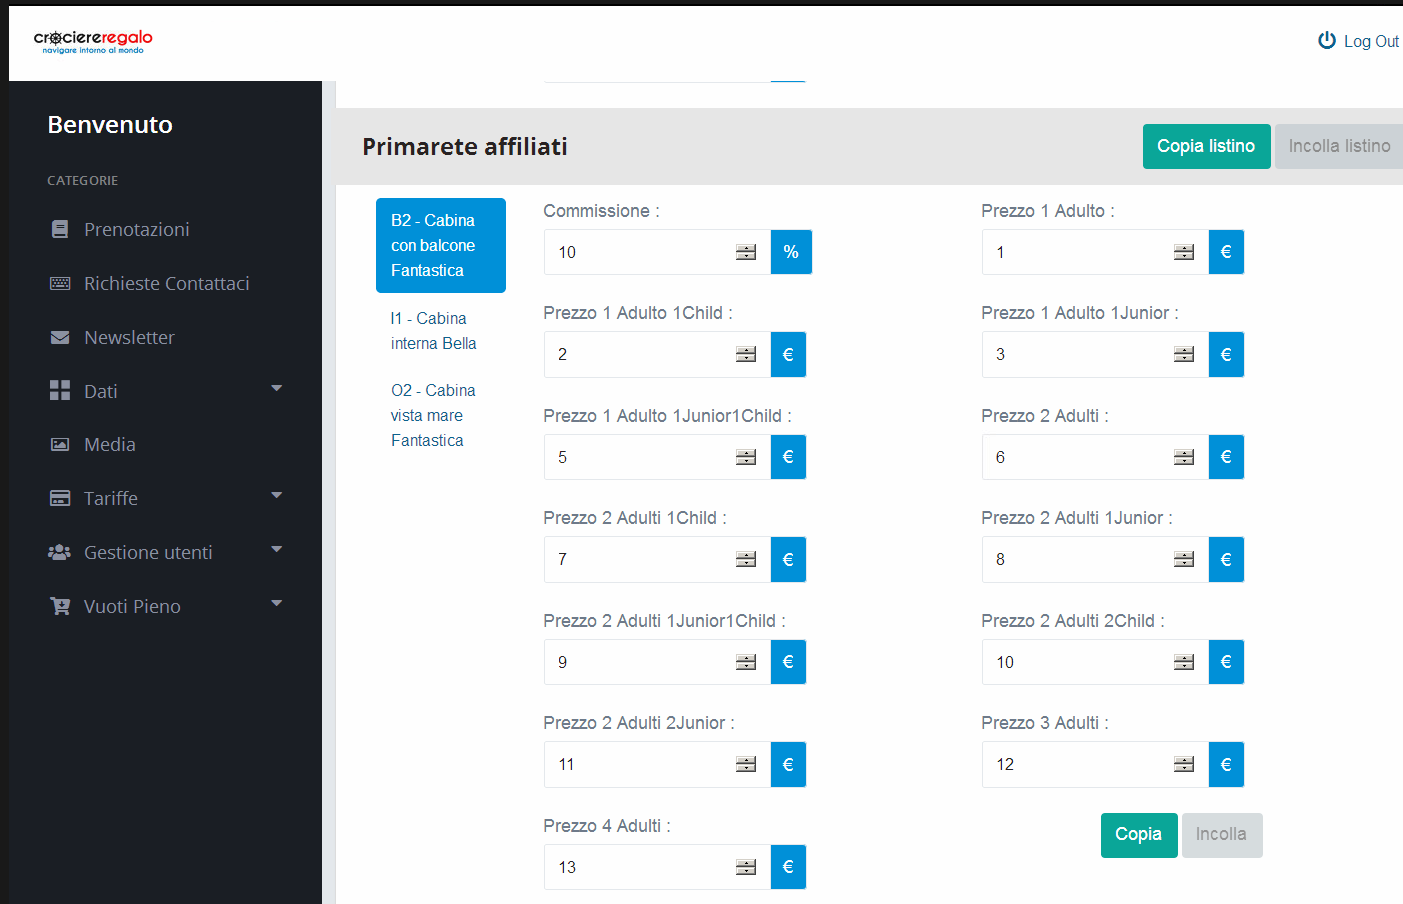
\includegraphics[width=1\columnwidth]{attivita/vuotopieno_prezzi} 
	\caption{Schermata di inserimento dei prezzi di un vuoto pieno.}
\end{figure}\\
I prezzi poi vengono salvati tramite una chiamata \gls{ajax} che invoca il metodo \textit{salvaPrezzi} del controller \textit{Back} precedentemente descritto.

\subsubsection{Inserimento della tariffa nel flusso di prenotazione}
Come già accennato nella \hyperref[section:flusso-prenotazione]{sezione \ref*{section:flusso-prenotazione}}, il flusso di prenotazione si compone di 6 step, a ciascuno dei quali corrisponde un metodo nel controller \textbf{WS\_Cruises} del \textit{dataExchange}. Questi 6 metodi venivano (e vengono tuttora) chiamati tramite richieste \gls{ajax} dal frontend e al loro interno chiamavano l'omologo metodo in grado di interfacciarsi con i \gls{webservice} del fornitore considerato.\\
Sono stati quindi creati i seguenti metodi:
\begin{center}
	\def\arraystretch{1.5}
	\begin{longtable}{ >{\raggedright}p{5.5cm} p{6.8cm}} 
		\hline
		\textbf{Metodo} & \textbf{Descrizione} \\ \hline
		+ Inventory\_categoryAvailabilty (inout wsResult:array) : void & Concatena al risultato eventualmente restituito dai \gls{webservice} del fornitore le categorie di cabine, se presenti, aventi tariffa vuoto per pieno. Il codice della tariffa restituita (dato che servirà alle successive funzioni) è "INVENTORY".\\
		\hline
		+ Inventory\_cabinAvailabilty () : array & Legge dal database (facendo delle query su Cruises\_Inventory, Cruises\_InventoryDetail e Cruises\_InventoryPrices) e restituisce le singole cabine disponibili, compreso il prezzo, secondo i qualificatori che legge dal payload della richiesta, quali numero ed età dei passeggeri, cruiseID considerato, categoria delle cabine di cui si vuole controllare la disponibilità e listino di appartenenza dell'utente.\\
		\hline
		+ Inventory\_requestPricing () : array & Calcola un preventivo in base ai parametri passati nel payload della richiesta, ovvero fornitore, cruiseID, numero della cabina, dati anagrafici dei passeggeri.\\
		\hline
		+ Inventory\_requestBooking () : string & Prenota la cabina passata come parametro nel payload della richiesta e ritorna il bookingID (identificativo della prenotazione) corrispondente.\\
		\hline
		+ Inventory \_requestBookingInformation (bookId: string) : array & Dato il bookId passato come parametro, restituisce tutti i dettagli inerenti alla prenotazione. \\
		\hline
	\end{longtable}
\end{center}
Il primo metodo del flusso, \textit{categoryAvailability}, in base al valore del parametro \textit{supplier} (letto dal payload della richiesta), invocava i metodi \textit{MSC\_categoryAvailability} o \textit{Costa\_categoryAvailability}, che interrogano i rispettivi \glspl{webservice}. È stato sufficiente quindi che il nuovo metodo creato \textit{Inventory\_categoryAvailabilty} venisse invocato da \textit{categoryAvailabilty} a prescindere dal \textit{supplier}, concatenando all'output dei metodi \textit{MSC\_categoryAvailability} o \textit{Costa\_categoryAvailability} le categorie di cabine eventualmente disponibili con tariffa vuoto per pieno.\\
Nei metodi \textit{cabinAvailability}, \textit{requestPricing}, \textit{requestBooking} e \textit{requestBookingInformation}, è stata introdotta un'istruzione condizionale che, in base al \textbf{fareCode} (codice della tariffa) passato come parametro, decida se invocare l'omologo metodo che legga dal database delle tariffe vuoto per pieno (in caso di fareCode = "INVENTORY") o dai \glspl{webservice} del fornitore.\\
Al frontend, infine, non è stato necessario fare alcuna modifica.
\subsubsection{Test}
Al termine della realizzazione, sono stati effettuati test manuali sulla congruenza dei dati tra le nuove tabelle e i vuoti pieno importati. 
Infine si è verificato che i dati presenti nelle tabelle fossero interpretati in maniera adeguata dalle varie query presenti nel flusso di prenotazione, dal primo all'ultimo dei sei step.
\newpage
\section{Aggiunta delle tariffe di un nuovo fornitore}
\subsection{Il problema}
L'ultimo argomento affrontato durante lo stage è stato aggiungere la possibilità di prenotare una crociera con \textit{Royal Caribbean},\textit{Celebrity} e \textit{Azamara}. Queste tre compagnie, per fortuna, forniscono, grazie alla società \textit{ISTINFOR}, dei \glspl{webservice} chiamati \textbf{FIBOS}, che sono unici per le tre compagnie di crociera sopra citate. \\
\textit{FIBOS} prevede l'utilizzo di due tipologie di \glspl{webservice}: \textbf{FDF} (Fibos Data Feed) e \textbf{RCCL} (Royal Caribbean Cruise Line).
\subsubsection{Importazione di aree geografiche, navi, porti e categorie di cabine}
Per poter interfacciarsi con i \glspl{webservice}, è stato necessario aggiungere al \bookingEngine\hphantom{i}le informazioni (codici, descrizioni) di aree geografiche, navi, porti e categorie di cabine utilizzate da FIBOS.

\subsubsection{Implementazione di FDF}
Questi \glspl{webservice} sono progettati per il trasferimento di grandi quantità di dati e forniscono un sistema di ricerca di crociere (e relativi prezzi). Si sono quindi dimostrati adatti al meccanismo di integrazione schedulata presente nel \bookingEngine. È stato dunque necessario creare un sistema che interrogasse i \glspl{webservice} \textit{FDF}, consolidandone i risultati nel \textit{DataExchange} ed integrandoli poi nell'\textit{OTA}. 

\subsubsection{Implementazione di RCCL}
Per far fronte ai dati richiesti in tempo reale dal flusso di prenotazione, invece, sono stati offerti da \textit{FIBOS} i \glspl{webservice} \textbf{RCCL}, che è stato necessario integrare ed interrogare.

\section{La soluzione}
\subsubsection{Importazione di aree geografiche, navi, porti e categorie di cabine}
Informazioni circa codici di aree geografiche, navi, porti, categorie di cabine, ponti ci sono state fornite da \textit{ISTINFOR} in un file formato \textit{.xlsx}. In caso di variazioni di tali informazioni, per contratto, ci sarebbe stato mandato un nuovo file aggiornato. Proprio per questo é stato deciso, invece di importare a mano i dati, di realizzare un importatore.\\
A livello grafico, è stata realizzata una semplice finestra di dialogo che permettesse di caricare il file in oggetto e mandarlo al backend per l'elaborazione.
\begin{figure}[!h] 
	\centering 
	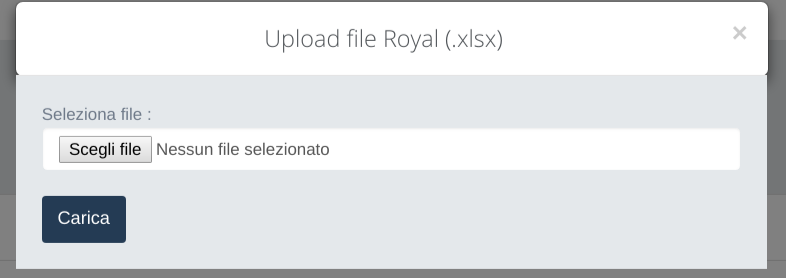
\includegraphics[width=.6\columnwidth]{attivita/upload_royal} 
	\caption{Schermata di caricamento del file passato da ISTINFOR}
\end{figure} \\
A livello backend, è stato realizzato un nuovo model nella parte \textit{OTA}, chiamato semplicemente \textit{Royal}, avente i seguenti metodi:

\begin{center}
	\def\arraystretch{1.5}
	\begin{longtable}{ >{\raggedright}p{5.5cm} p{6.8cm}} 
		\hline
		\textbf{Metodo} & \textbf{Descrizione} \\ \hline
		+ parse(fileName: string) : boolean & Elabora il file avente nome (e percorso) 'fileName'. Restituisce true se l'elaborazione è andata a buon fine, false altrimenti .\\
		\hline
		- loadPorts () : boolean & Viene invocato da \textit{parse}, si occupa di leggere i porti dal file e caricarli nella tabella \textit{Cruises\_Ports} del \textit{DataExchange} (che poi viene sincronizzata, ad ogni integrazione, con l'omonima tabella dell'\textit{OTA}). Restitusce \textit{true} in caso di successo, \textit{false} altrimenti.\\
		\hline
		- loadShips () : boolean & Viene invocato da \textit{parse}, si occupa di leggere le navi dal file e caricarle nella tabella \textit{Cruises\_Ships} del \textit{DataExchange} (che poi viene sincronizzata, ad ogni integrazione, con l'omonima tabella dell'\textit{OTA}). Restitusce \textit{true} in caso di successo, \textit{false} altrimenti.\\
		\hline
		- loadDecks () : boolean & Viene invocato da \textit{parse}, si occupa di leggere i ponti delle varie navi dal file e caricarli nella tabella \textit{Cruises\_Decks} del \textit{DataExchange} (che poi viene sincronizzata, ad ogni integrazione, con l'omonima tabella dell'\textit{OTA}). Restitusce \textit{true} in caso di successo, \textit{false} altrimenti.\\
		\hline
		- loadCategories () : boolean & Viene invocato da \textit{parse}, si occupa di leggere le categorie di cabine delle varie navi dal file e caricarle nella tabella \textit{Cruises\_CabinCategories} del \textit{DataExchange} (che poi viene sincronizzata, ad ogni integrazione, con l'omonima tabella dell'\textit{OTA}). Restitusce \textit{true} in caso di successo, \textit{false} altrimenti.\\
		\hline
	\end{longtable}
\end{center}
È stato poi creato un nuovo metodo \textit{caricaRoyal} sul controller \textit{Back} dell'\textit{OTA}, che prende il file caricato dal frontend e lo passa al metodo \textit{parse} del model \textit{Royal} sopra descritto.

\subsubsection{Implementazione di FDF}
Nel file \textit{.xlsx} fornito da \textit{ISTINFOR} mancano tutte le informazioni inerenti a itinerari, prezzi e partenze delle crociere. Queste sono invece fornite dal \gls{webservice} \textbf{FDF}, che quindi si è dovuto implementare. L'interazione con tale \gls{webservice} avviene tramite chiamate \gls{SOAP} ad appositi URL forniti da \textit{ISTINFOR}.\\ Essendoci stati forniti solo degli URL di sviluppo, le chiamate restituiscono dati verosimili ma non veri. Inoltre, \textit{ISTINFOR} utilizza un firewall: vengono accettate richieste provenienti solo da IP noti. Siccome il server di sviluppo utilizzato era all'interno della rete dell'ufficio, con IP dinamico e non esposto, è stato necessario creare un ambiente online di test, da affiancare a quello di produzione (all'indirizzo \url{http://primaretetest.webpd.it/crociereregalo} e \url{http://primaretetest.webpd.it/dataExchange}).\\
Premesso ciò, la struttura di una chiamata \gls{SOAP} accettata da \textit{FDF} è la seguente:
\begin{lstlisting}
<SOAP-ENV:Envelope xmlns:SOAP-ENV="http://schemas.xmlsoap.org/soap/envelope/" xmlns:ns1="http://tempuri.org/WebService/Service1">
  <SOAP-ENV:Body>
    <ns1:PROCEDURA>
      <ns1:MessageXML>
        <PROCEDURA>
          <Header>
            <CruiseLineCode>RCCL</CruiseLineCode>
            <SubsystemId>2</SubsystemId>
            <AgencyId1>041178383</AgencyId1>
            <AgencyId2>041178383</AgencyId2>
            <Currency>EUR</Currency>
            <AgencyConsumer>A</AgencyConsumer>
          </Header>
          <PROCEDURA>
            <PARAMETRO/>
          </PROCEDURA>
        </PROCEDURA>
      </ns1:MessageXML>
    </ns1:PROCEDURA>
  </SOAP-ENV:Body>
</SOAP-ENV:Envelope>
\end{lstlisting}Il tag \textit{Header} ed il suo contenuto sono comuni a tutte le richieste. Bisogna poi sostituire il nome \textit{PROCEDURA} con quello della funzione che si vuole invocare (ad esempio \textit{SearchBySea}) e, in base a quanto definito nella documentazione, includere una lista di parametri (allo stesso livello del tag \textit{Parametro}). Prima di invocare una procedura generica, però, è necessario fare una chiamata alla funzione di login, che permette di autenticarsi.
Tutte le chiamate ai \gls{webservice} vengono gestite dal \textit{DataExchange}, all'interno del quale sono state create due nuove classi per semplificarne l'interazione: \textit{Royal\_Model} e \textit{Royal\_WS}.\\
La prima è un model che serve ad effettuare le chiamate ai \gls{webservice} forniti, e si compone dei seguenti metodi:
\begin{center}
	\def\arraystretch{1.5}
	\begin{longtable}{ >{\raggedright}p{5.5cm} p{6.8cm}} 
		\hline
		\textbf{Metodo} & \textbf{Descrizione} \\
		\hline
		- buildHeader(lineCode: string) : void & Costruisce e salva in una variabile interna alla classe l'intestazione della richiesta, popolando contenuto il tag \textit{<CruiseLineCode>} con il valore del parametro \textit{lineCode} passato.\\
		\hline
		- callWS (xml: string, function: string) : SimpleXMLObject & Fa una richiesta al \gls{webservice}, chiamando la procedura remota \textit{function}, utilizzando come payload il valore del parametro \textit{xml}. Restituisce la risposta del \gls{webservice} come istanza di SimpleXMLObject (che permette di muoversi agevolmente tra i vari tag e attributi), oppure NULL in caso si verifichi un errore di parsing (ad esempio la risposta non sia in XML ben formattato).\\
		\hline
		+ login (lineCode: string) : boolean & Effettua la chiamata alla procedura remota di login, avvalendosi della funzione \textit{buildHeader}, alla quale viene passato il parametro \textit{lineCode}.\\
		\hline
		+ requestPricesSea (sea: string, date: string, guests: int) : SimpleXMLObject & Effettua una \gls{RPC} al metodo \textit{RequestSearchBySeaPricing} del \gls{webservice}, con i parametri \textit{Sea}, \textit{Date} e \textit{Guests} valorizzati in base a quanto passato.\\
		\hline
	\end{longtable}
\end{center}
Il metodo \textit{RequestSearchBySeaPricing} di \textit{FDF} permette di effettuare una ricerca del miglior prezzo per ogni categoria di cabina di tutte le partenze di tutte le navi gestite dal sistema (quindi Royal, Celebrity e Azamara). Nella ricerca possono essere inserite delle restrizioni sul numero di passeggeri, sull'area geografica (mare) di navigazione e su un intervallo di date (ad esempio crociere che partono dal 3 settembre 2018 al 10 ottobre 2019). \\
La chiamata a \textit{RequestSearchBySeaPricing} (quindi al metodo \textit{requestPricesSea} di \textit{Royal\_Model}) viene utilizzata dal meccanismo schedulato di integrazione per popolare le informazioni inerenti agli itinerari disponibili, alle date di partenza di ogni itinerario e ai prezzi di ogni categoria di cabina di ogni data di partenza di ogni itinerario. Tale elaborazione richiede molto tempo (fino a 40 minuti), per tanto viene eseguita durante la notte (è stato deciso di schedularla alle 2 del mattino, dato che non c'é un orario preciso di rilascio dei nuovi aggiornamenti). \\
Per permettere l'invocazione di tale metodo è stato realizzato un controller apposito, chiamato \textit{Royal\_WS}, il cui contenuto é il seguente:
\begin{center}
	\def\arraystretch{1.5}
	\begin{longtable}{ >{\raggedright}p{5.5cm} p{6.8cm}} 
		\hline
		\textbf{Metodo} & \textbf{Descrizione} \\
		\hline
		+ load\_PricesSea() : void & Tramite la chiamata al metodo \textit{requestPricesSea} del model \textit{Royal\_Model}, sincronizza, per ogni itinerario, la lista delle partenze (incluse disponibilità di cabine, prezzi e in generale tutto quanto restituito dalla funzione) con il database del \textit{DataExchange}. Grazie al meccanismo dei \textit{magic method} descritto in sezione \ref{section:struttura-codice}, esso può essere invocato direttamente via URL.\\
		\hline
	\end{longtable}
\end{center}

\subsubsection{Implementazione di RCCL}
Il metodo \textit{RequestSearchBySeaPricing} di \textit{FDF}, ai fini dell'integrazione dati, presentava un grande difetto: non restituiva il dettaglio dell'itinerario, ma vi si riferiva utilizzandone solo il codice. Ciò rappresentava un problema sia ai fini della ricerca offerta dal \bookingEngine\hphantom{i}che della visualizzazione dei dettagli di una crociera. In tale pagina, infatti, è presente la lista di destinazioni toccate dalla crociera. Per reperire queste informazioni si sarebbe potuto mappare a mano ciascun itinerario in base alle informazioni contenute nei cataloghi cartacei delle tre compagnie, ma sarebbe stato un lavoro enorme (gli itinerari sono circa 1400 in totale) che si sarebbe dovuto ripetere costantemente nel tempo, in quanto essi cambiano ogni manciata di mesi.\\
Per, dunque, evitare tanto lavoro si è deciso di implementare, all'interno del metodo \textit{load\_PricesSea} della classe \textit{Royal\_WS}, delle \gls{RPC} a \textit{RequestItinerary}, fornito dal \gls{webservice} \textit{RCCL}, che restituisce le informazioni dettagliate dell'itinerario corrispondente ai parametri passati (codice della nave, data di partenza e codice itinerario).  Dato che il protocollo di comunicazione è analogo a quello utilizzato per \textit{FDF}, si è deciso (per questo e per tutti le altre \gls{RPC} utilizzate di \textit{RCCL}) di riutilizzare la classe \textit{Royal\_Model}, andando a definire nuovi metodi in base alle necessità. In questo caso è stato aggiunto il seguente metodo: 
\begin{center}
	\def\arraystretch{1.5}
	\begin{longtable}{ >{\raggedright}p{5.5cm} p{6.8cm}} 
		\hline
		\textbf{Metodo} & \textbf{Descrizione} \\
		\hline
		+ requestItinerary(ship: string, date: string, itinerary: string) : SimpleXMLObject & Effettua una \gls{RPC} a \textit{RequestItinerary} del \gls{webservice}, con i parametri \textit{Ship}, \textit{Date} e \textit{Itinerary} valorizzati in base a quanto passato. Ritorna la risposta in forma di oggetto SimpleXMLObject, o NULL in caso di risposta mal formattata.\\
		\hline
	\end{longtable}
\end{center}
\begin{figure}[!h] 
	\centering 
	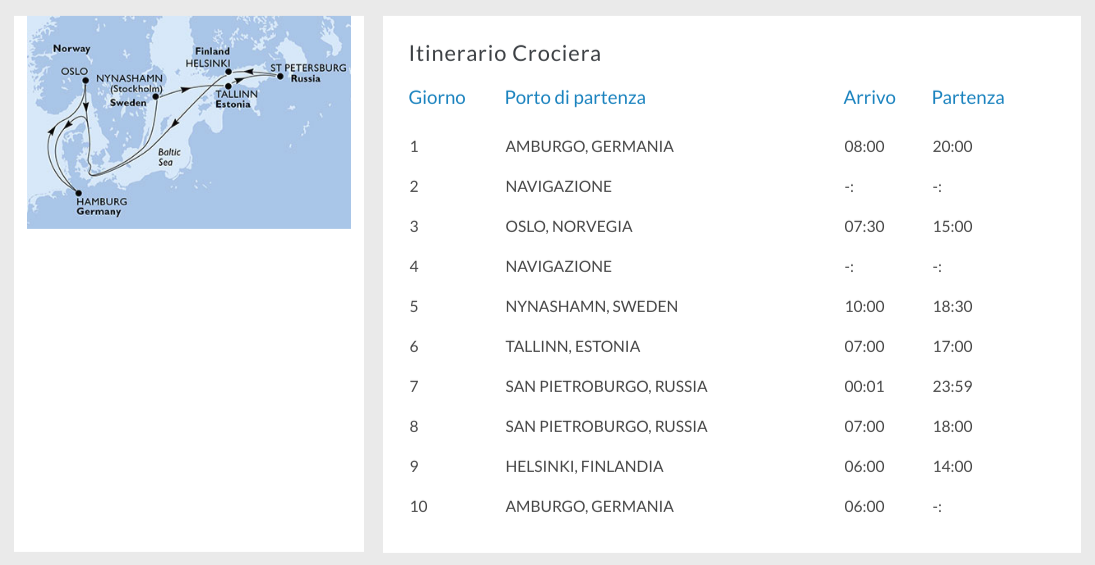
\includegraphics[width=.9\columnwidth]{attivita/dettaglio_itinerario} 
	\caption{Dettaglio dell'itinerario visualizzato dal frontend.}
\end{figure}
Le informazioni ritornate da questo metodo includono anche la lista di destinazioni dell'itinerario, ma la lingua in cui i nomi di tali destinazioni (porti, città, stati) vengono restituiti è mista. Ad esempio, per riferirsi alle isole delle Azzorre, viene usato tanto il nome italiano "Azzorre" quanto il nome spagnolo "Azores". La stessa cosa vale per Danimarca, Scozia, Australia, Emirati Arabi, Canarie, Belgio ecc. È stato dunque necessario realizzare un mapping manuale dei nomi, che permettesse di tradurre i nomi in lingua italiana.\\ \\
Per quanto riguarda l'integrazione nel flusso di prenotazione delle tariffe \textit{FIBOS}, analogamente al lavoro svolto per i vuoti pieno, sono stati creati ed implementati nuovi metodi nel controller \textit{WS\_Cruises} che utilizzano nuovi metodi creati nel model \textit{Royal\_Model}. Sono state utilizzate le seguenti procedure di \textit{RCCL}:

\begin{center}
	\def\arraystretch{1.5}
	\begin{longtable}{ >{\raggedright}p{5.5cm} p{6.8cm}} 
		\hline
		\textbf{Procedura} & \textbf{Descrizione} \\
		\hline
		RequestCategories & Dati in input nave (Ship), data di partenza (Date), numero ed età dei passeggeri (Guests), restituisce una lista di tariffe disponibili per quella partenza, complete di prezzi per ogni categoria di cabina, tasse portuali ed eventualmente oneri aggiuntivi.\\
		\hline
		RequestCabins &  Dati in input nave (Ship), data di partenza (Date), numero ed età dei passeggeri (Guests) e codice della tariffa (FareCode), restituisce una lista di cabine disponibili che soddisfano i criteri definiti dai parametri passati.\\
		\hline
		RequestPricing &  Dati in input nave (Ship), data di partenza (Date), numero ed età dei passeggeri (Guests), codice della tariffa (FareCode) e della cabina (Cabin), restituisce una quotazione veritiera che soddisfa i criteri definiti dai parametri passati.\\
		\hline
		RequestBooking &  Dati in input nave (Ship), data di partenza (Date), numero, età e dati anagrafici dei passeggeri (Guests), codice della tariffa (FareCode) e della cabina (Cabin) e la tipologia di prenotazione che si vuole effettuare (AgreementSt, da porre a OF in caso si voglia fare un'opzione, mentre a BK in caso di prenotazione vera e propria), restituisce il codice di prenotazione (BookingId), assieme all'ammontare di denaro e relative scadenze dei pagamenti.\\
		\hline
		RequestRetrieve &  Dato in input il numero di prenotazione (BookingId), restituisce le informazioni dettagliate (sia inerenti all'itinerario, sia allo stato dei pagamenti) della prenotazione corrispondente.\\
		\hline
	\end{longtable}
\end{center}
Per effettuare le \gls{RPC} sopra descritte, sono stati realizzati i seguenti nuovi metodi all'interno della classe \textit{Royal\_Model}:
\begin{center}
	\def\arraystretch{1.5}
	\begin{longtable}{ >{\raggedright}p{5.5cm} p{6.8cm}} 
		\hline
		\textbf{Metodo} & \textbf{Descrizione} \\
		\hline
		+ categoryAvailability(ship: string, date: string, guests: array) : SimpleXMLObject & Effettua una \gls{RPC} a \textit{RequestCategories} del \gls{webservice}, con i parametri \textit{Ship}, \textit{Date} e \textit{Guests} valorizzati in base a quanto passato. Ritorna la risposta in forma di oggetto SimpleXMLObject, o NULL in caso di risposta mal formattata.\\
		\hline
		+ cabinAvailability(ship: string, date: string, guests: array, fareCode: string) : SimpleXMLObject & Effettua una \gls{RPC} a \textit{RequestCabins} del \gls{webservice}, con i parametri \textit{Ship}, \textit{Date}, \textit{Guests}, \textit{FareCode} valorizzati in base a quanto passato. Ritorna la risposta in forma di oggetto SimpleXMLObject, o NULL in caso di risposta mal formattata.\\
		\hline
		+ pricingInformation(ship: string, date: string, cabin: string, fareCode: string, guest: array) : SimpleXMLObject & Effettua una \gls{RPC} a \textit{RequestPricing} del \gls{webservice}, con i parametri \textit{Ship}, \textit{Date}, \textit{Guests}, \textit{FareCode}, \textit{Cabin} valorizzati in base a quanto passato. Ritorna la risposta in forma di oggetto SimpleXMLObject, o NULL in caso di risposta mal formattata.\\
		\hline
		+ book(ship: string, date: string, cabin: string, fareCode: string, guest: array, agreementSt: string) : SimpleXMLObject & Effettua una \gls{RPC} a \textit{RequestBooking} del \gls{webservice}, con i parametri \textit{Ship}, \textit{Date}, \textit{Guests}, \textit{FareCode}, \textit{Cabin}, \textit{AgreementSt} valorizzati in base a quanto passato. Ritorna la risposta in forma di oggetto SimpleXMLObject, o NULL in caso di risposta mal formattata.\\
		\hline
		+ retrieveBooking(bookingNumber: string) : SimpleXMLObject & Effettua una \gls{RPC} a \textit{RequestRetrieve} del \gls{webservice}, con il parametro \textit{BookingId} valorizzato in base a quanto passato. Ritorna la risposta in forma di oggetto SimpleXMLObject, o NULL in caso di risposta mal formattata.\\
		\hline
	\end{longtable}
\end{center}
Infine, per invocare ed elaborare i risultati dei nuovi metodi scritti in \textit{Royal\_Model}, sono state aggiunte le seguenti funzioni a \textit{WS\_Cruises}:
\begin{center}
	\def\arraystretch{1.5}
	\begin{longtable}{ >{\raggedright}p{5.5cm} p{6.8cm}} 
		\hline
		\textbf{Metodo} & \textbf{Descrizione} \\
		\hline
		+ Fibos\_categoryAvailability (supplier: int, cruiseID: string, guest: array) : array & Restituisce un array contenente la lista delle categorie di cabina effettivamente disponibili, interrogando il \gls{webservice} tramite l'invocazione del metodo \textit{categoryAvailability} di \textit{Royal\_Model}.\\
		\hline
		+ Fibos\_cabinAvailability (supplier: int, cruiseID: string, guest: array, fareCode: string) : array & Restituisce un array contenente la lista delle singole cabina effettivamente disponibili, interrogando il \gls{webservice} tramite l'invocazione del metodo \textit{categoryAvailability} di \textit{Royal\_Model}, tenendo conto dei parametri passati (quindi anche del fareCode, ovvero della tariffa scelta allo step precedente).\\
		\hline
		+ Fibos\_requestPricing (supplier: int, cruiseID: string, guest: array, fareCode: string, cabin: string) : array & Restituisce un array contenente una quotazione veritiera per la cabina selezionata (tenendo conto di tariffa, crociera, cabina, selezionate e del numero ed età dei passeggeri), interrogando il \gls{webservice} tramite l'invocazione del metodo \textit{pricingInformation} di \textit{Royal\_Model}.\\
		\hline
		+ Fibos\_requestBooking (supplier: int, cruiseID: string, guest: array, fareCode: string, cabin: string, agreementSt: string) : array & Effettua una prenotazione in base ai parametri passati (tariffa, crociera, cabina, numero ed età dei passeggeri, tipo di prenotazione), interrogando il \gls{webservice} tramite l'invocazione del metodo \textit{book} di \textit{Royal\_Model}.\\
		\hline
		+ Fibos\_requestBookingInformation (bookingNumber: string) : array & Restituisce le informazioni inerenti alla prenotazione passata come parametro, interrogando il \gls{webservice} tramite l'invocazione del metodo \textit{retrieveBooking} di \textit{Royal\_Model}.\\
		\hline
	\end{longtable}
\end{center}

\subsubsection{Problemi riscontrati}
Nell'implementazione dei due \glspl{webservice} sopra menzionati, sono stati riscontrati dei problemi, principalmente con la documentazione fornitaci da \textit{ISTINFOR}. All'inizio, infatti, ci sono stati forniti i manuali aggiornati a febbraio 2014, e molti parametri delle procedure da noi usate non corrispondevano a quanto scritto nel manuale. Dopo numerose sollecitazioni, siamo riusciti ad ottenere la guida aggiornata all'ultima release (febbraio 2018).\\
Un altro problema riscontrato, forse quello che ci ha fatto perdere più tempo, é stato l'eterogeneità dei formati delle date richiesti dai parametri/tag/attributi delle varie procedure. Infatti, alcune di esse richiedevano che la data fosse espressa in formato YYYY-mm-dd (ovvero 2018-09-27), altre in formato YYYYmmdd (20180927), altre ancora in formato dd/mm/YYYYY (27/09/2018) o addirittura mm/dd/YYYY (09/27/2018). Al di là delle numerose conversioni necessarie per adattarle al formato presente nel database (che é YYYY-mm-dd), il problema è stato che il manuale si è rivelato ambiguo riguardo al formato corretto da usare (o non veniva specificato o, addirittura, veniva specificato sbagliato). Visto anche l'elevato tempo di risposta (settimane) del supporto tecnico, soprattutto probabilmente perché lo stage si è svolto durante il periodo estivo tipico delle ferie, abbiamo dovuto procedere molto spesso per tentativi, perdendo molto tempo.

\subsubsection{Test}
Anche in questo caso, vista l'assenza di una suite di testing, si sono svolte delle verifiche a mano di congruenza tra i dati restituiti da i \gls{webservice} e quelli presenti nel database. Inoltre, grazie alle credenziali di accesso forniteci da \textit{Primarete}, è stato possibile verificare la congruenza tra quanto presente nel database e quanto visualizzato dal portale di prenotazione ufficiale del gruppo Royal/Celebrity/Azamara. I dati in nostro possesso, sebbene derivanti da canali di test e non di produzione, erano in pratica dati reali, solo semplicemente non aggiornatissimi.             % Concept Preview
%% !TEX encoding = UTF-8
% !TEX TS-program = pdflatex
% !TEX root = ../tesi.tex

%**************************************************************
\chapter{Progettazione e codifica}
\label{cap:progettazione-codifica}
%**************************************************************

\intro{Breve introduzione al capitolo}\\

%**************************************************************
\section{Tecnologie e strumenti}
\label{sec:tecnologie-strumenti}

Di seguito viene data una panoramica delle tecnologie e strumenti utilizzati.

\subsection*{Tecnologia 1}
Descrizione Tecnologia 1.

\subsection*{Tecnologia 2}
Descrizione Tecnologia 2

%**************************************************************
\section{Ciclo di vita del software}
\label{sec:ciclo-vita-software}

%**************************************************************
\section{Progettazione}
\label{sec:progettazione}

\subsubsection{Namespace 1} %**************************
Descrizione namespace 1.

\begin{namespacedesc}
    \classdesc{Classe 1}{Descrizione classe 1}
    \classdesc{Classe 2}{Descrizione classe 2}
\end{namespacedesc}


%**************************************************************
\section{Design Pattern utilizzati}

%**************************************************************
\section{Codifica}
             % Product Prototype
%% !TEX encoding = UTF-8
% !TEX TS-program = pdflatex
% !TEX root = ../tesi.tex

%**************************************************************
\chapter{Verifica e validazione}
\label{cap:verifica-validazione}
%**************************************************************             % Product Design Freeze e SOP
% !TEX encoding = UTF-8
% !TEX TS-program = pdflatex
% !TEX root = ../tesi.tex

%**************************************************************
\chapter{Conclusioni}
\label{cap:conclusioni}
%**************************************************************

%**************************************************************
\section{Raggiungimento degli obiettivi}
La pianificazione in termine di ore totali è stata perfettamente rispettata: lo stage si è svolto in 310 ore, rispettando le scadenze settimanali pianificate nella sezione \ref{sec:vincoli-temporali}. Ciò, purtroppo, significa che non c'è stato spazio per lo svolgimento delle attività \textbf{opzionali} descritte sezione \ref{section:altri-interventi-minori}.\\Riassumendo, lo stato di soddisfacimento degli obiettivi è stato dunque il seguente:
\begin{center}
	\def\arraystretch{1.5}
	\begin{longtable}{p{1.5cm} p{8.5cm} p{1.5cm} } 
		\hline
		\multicolumn{2}{c}{\textbf{Obbligatori}} & Soddisfatto\\
		\hline
		Ob1 & Interazione con il database SQL Server attraverso le librerie del \gls{framework} Codeigniter & Si\\
		\hline
		Ob2 & Realizzazione integrazione flat-file di un nuovo fornitore con il Data Exchange del \bookingEngine & Si\\
		\hline
		Ob3 & Aggiunta prodotti e tariffe del nuovo fornitore ai risultati della ricerca lato Front-End del \bookingEngine & Si\\
		\hline
		Ob4 & Esecuzione test e redazione documentazione sul lavoro svolto & Si\\
		\hline
		\multicolumn{2}{c}{\textbf{Desiderabili}} & Soddisfatto\\
		\hline
		D1 & Realizzazione del registro carichi/scarichi tariffe “vuoto per pieno” come	funzionalità lato Back-End del \bookingEngine & Si\\
		\hline
		D2 & Interrogazione web-service in tempo reale per sincronizzare prezzi e disponibilità del nuovo fornitore con il Data Exchange & Si\\
		\hline
		D3 & Realizzazione conferma prenotazione al fornitore come funzionalità lato Front-End del \bookingEngine & Si\\
		\hline
		\multicolumn{2}{c}{\textbf{Opzionali}} & Soddisfatto\\
		\hline
		Op1 & Analisi e realizzazione di nuove funzionalità & No\\
		\hline
	\end{longtable}
\end{center}
Avendo raggiunto tutti gli obiettivi obbligatori e desiderabili prefissati, considero l'esito dello stage più che soddisfacente, anche perché buona parte del codice da me sviluppato è stato portato direttamente in produzione.
%**************************************************************
\section{Competenze acquisite}
\subsection{Competenze tecnologiche}
A livello tecnologico, non ho acquisito grandi nuove conoscenze, data anche la mia esperienza pregressa in questo campo.\\ Ho avuto modo di interagire con il \gls{framework} \textit{Codeigniter}, che devo dire ho imparato ad apprezzare molto, soprattutto per la sua semplicità. Posso sicuramente affermare che riutilizzerò questo \gls{framework} nei prossimi progetti in PHP che andrò a realizzare. Ho avuto anche l'occasione di interfacciarmi con \textit{Microsoft SQL Server} che però, ai fin dei conti, non differisce poi più di tanto rispetto agli altri \gls{DBMS} da me già utilizzati in passato.
\subsection{Competenze metodologiche}
A livello metodologico, invece, posso affermare di aver ricevuto un grande valore aggiunto da questa esperienza. Ho potuto "toccare con mano" cosa significhi lavorare con metodo, ed i vantaggi che ciò porta a livello di produttività. Infatti, avere del metodo di lavoro, permette di realizzare prodotti aventi più alta qualità, che rispondono in modo più affine alle esigenze del committente. Ho anche potuto riscontrare come il modello evolutivo descritto in sezione \ref{sec:modello-evolutivo} permetta di rispondere molto bene alle esigenze mutevoli del mercato (anzi, sarebbe meglio dire del committente tipicamente indeciso). Posso dunque affermare di aver acquisito una \textit{way-of-working} che sicuramente andrò ad applicare ai miei progetti "amatoriali" che sto attualmente portando avanti.
%**************************************************************
\section{Valutazione sul rapporto azienda-università}
Ho iniziato a programmare da completo autodidatta. La scuola superiore che ho frequentato ha contribuito a darmi un'infarinatura accademica riguardo il mondo dell'informatica, ma sono sempre stato un cosiddetto "smanettone". Per imparare qualcosa, ho sempre prediletto l'aspetto pratico a quello teorico, perché permette di ricevere subito un frutto remunerativo del proprio lavoro. All'inizio del percorso della laurea triennale, devo dire di essere rimasto un po' deluso dall'eccessivo (a mio parere dell'epoca) approccio teorico nello studio di questa materia. Con l'avanzare del tempo, però, ho imparato che (almeno il più delle volte) è utile capire quello che si sta facendo, e per capirlo è necessario valutare anche l'approccio teorico al problema che si sta cercando di risolvere.\\
A posteriori, ora che, con la discussione di questo documento, ho concluso il mio percorso di laurea triennale, penso che l'approccio teorico offerto da questo corso di laurea possa giovare a tanti "smanettoni" come me, anche perché il mondo dell'informatica si evolve ad una velocità molto elevata, che rende molto difficile starne al passo. Ritengo tuttavia sarebbe una buona idea avviare collaborazioni, nel limite del possibile, con "entità esterne all'aula" (aziende, istituzioni) per lo svolgimento dei progetti tipici di alcuni corsi (ad esempio Tecnologie Web). Così facendo, probabilmente, si avrebbero degli studenti più abili nella risoluzione di problemi "reali", preparati ad affrontare il mondo del lavoro e sarebbe data loro la possibilità di esplorare tecnologie magari innovative ma sempre affini al corso (ad esempio Node.js), un po' come accade già con Ingegneria del Software. Probabilmente, infine, sarebbe anche più motivante per gli studenti stessi, in quanto realizzerebbero qualcosa di non fine a se stesso.             % Conclusioni
%\appendix                               
%% !TEX encoding = UTF-8
% !TEX TS-program = pdflatex
% !TEX root = ../tesi.tex

%**************************************************************
\chapter{Appendice A}
%**************************************************************

\epigraph{Citazione}{Autore della citazione}



             % Appendice A

%**************************************************************
% Materiale finale
%**************************************************************
\backmatter
\printglossaries
% !TEX encoding = UTF-8
% !TEX TS-program = pdflatex
% !TEX root = ../tesi.tex

%**************************************************************
% Bibliografia
%**************************************************************
\cleardoublepage
\begin{thebibliography}{99}
	\bibitem{sqlserverpricing}
		\textit{Prezzi di SQL Server - consultato 13/09/2018}
		\url{https://bit.ly/2rECrAS}
\end{thebibliography}


\end{document}
